\documentclass[cn,10pt,math=newtx,citestyle=gb7714-2015,bibstyle=gb7714-2015]{elegantbook}

\usepackage{polynom}
\usepackage{float}

\title{历年 CSP 题目解析}
\subtitle{仅为参考练习所用}

\author{lonlyn}
\institute{Shanxi University Algorithm Group}
\date{December 30, 2021}
\version{1.0}

\setcounter{tocdepth}{3}

\cover{cover.jpg}

\newif\ifonlyanalyze % 是否只有分析,没有题面
% \onlyanalyzefalse % 题面+分析
\onlyanalyzetrue % 只有分析,没有题面

% 本文档命令
\usepackage{array}
\newcommand{\ccr}[1]{\makecell{{\color{#1}\rule{1cm}{1cm}}}}

\definecolor{customcolor}{RGB}{32,178,170}
\colorlet{coverlinecolor}{customcolor}



\begin{document}

\maketitle
\frontmatter

\chapter*{特别声明}

\markboth{Introduction}{前言}

该书仅供内部学习使用,如果有侵权请联系作者。

信息学竞赛的发展,吸引越来越多的人加入了“卷”的行列。CCF CSP的历年题解在网上也是随处可见,但题解质量参差不齐。很多题解只有标准答案,缺少题目分析;更有甚者无法通过答案,充满了分号大小写问题等错误。

本书的目的是为了实现以下几点:

\begin{itemize}
  \item 提供规范的代码程序。这里的规范,既要具有程序的可读性,也要具备考场的简易性。
  \item 提供多样的解题思路。有些时候,网上的大佬往往一语道破问题求解的思路,但怎么想到的却往往不提。这里力求从部分分开始,逐渐深入,汇集众人智慧,逐步解决难题。
  \item 提供筛选的额外补充。做一道题的目的不是只做一道题,而是可以做到举一反三,但我们常常忽略这一点。
\end{itemize}

感谢 \href{https://github.com/ElegantLaTeX/ElegantBook}{Elegant\LaTeX{}} 提供如此精美的模板,希望这本书能够给大家带来帮助。

\vskip 1.5cm

\begin{flushright}
  lonlyn\\
  December 30, 2021
\end{flushright}

\tableofcontents

\mainmatter

\chapter{CCF CSP认证总览}

待补充。

% \chapter{第1次认证(2014年03月)}

% \section{题目及设计知识点}

% % \section{201403-1}

% \input{problem/1/201403-1-p.tex}

% % \section{201403-2}

% \input{problem/1/201403-2-p.tex}

% % \section{201403-3}

% \input{problem/1/201403-3-p.tex}

% % \section{201403-4}

% \input{problem/1/201403-4-p.tex}

% % \section{201403-5}

% \input{problem/1/201403-5-p.tex}

% \chapter{第2次认证(2014年09月)}

% \section{题目及设计知识点}

% % \section{201409-1}

% \input{problem/2/201409-1-p.tex}

% % \section{201409-2}

% \input{problem/2/201409-2-p.tex}

% % \section{201409-3}

% \input{problem/2/201409-3-p.tex}

% % \section{201409-4}

% \input{problem/2/201409-4-p.tex}

% % \section{201409-5}

% \input{problem/2/201409-5-p.tex} 

% \chapter{第3次认证(2014年12月)}

% \section{题目及设计知识点}

% % \section{201412-1}

% \input{problem/3/201412-1-p.tex}

% % \section{201412-2}

% \input{problem/3/201412-2-p.tex}

% % \section{201412-3}

% \input{problem/3/201412-3-p.tex}

% % \section{201412-4}

% \input{problem/3/201412-4-p.tex}

% % \section{201412-5}

% \input{problem/3/201412-5-p.tex}

% \chapter{第4次认证(2015年03月)}

% \section{题目及设计知识点}

% % \section{201503-1}

% \input{problem/4/201503-1-p.tex}

% % \section{201503-2}

% \input{problem/4/201503-2-p.tex}

% % \section{201503-3}

% \input{problem/4/201503-3-p.tex}

% % \section{201503-4}

% \input{problem/4/201503-4-p.tex}

% % \section{201503-5}

% \input{problem/4/201503-5-p.tex}

% \chapter{第5次认证(2015年09月)}

% \section{题目及设计知识点}

% % \section{201509-1}

% \input{problem/5/201509-1-p.tex}

% % \section{201509-2}

% \input{problem/5/201509-2-p.tex} 

% % \section{201509-3}

% \input{problem/5/201509-3-p.tex}

% % \section{201509-4}

% \input{problem/5/201509-4-p.tex}

% % \section{201509-5}

% \input{problem/5/201509-5-p.tex}

% \chapter{第6次认证(2015年12月)}

% \section{题目及设计知识点}

% % \section{201512-1}

% \input{problem/6/201512-1-p.tex} 

% % \section{201512-2}

% \input{problem/6/201512-2-p.tex}

% % \section{201512-3}

% \input{problem/6/201512-3-p.tex}

% % \section{201512-4}

% \input{problem/6/201512-4-p.tex}

% % \section{201512-5}

% \input{problem/6/201512-5-p.tex}

% \chapter{第7次认证(2016年04月)}

% \section{题目及设计知识点}

% % \section{201604-1}

% \input{problem/7/201604-1-p.tex}

% % \section{201604-2}

% \input{problem/7/201604-2-p.tex}

% % \section{201604-3}

% \input{problem/7/201604-3-p.tex}

% % \section{201604-4}

% \input{problem/7/201604-4-p.tex}

% % \section{201604-5}

% \input{problem/7/201604-5-p.tex}

% \chapter{第8次认证(2016年09月)}

% \section{题目及设计知识点}

% % \section{201609-1}

% \input{problem/8/201609-1-p.tex}

% % \section{201609-2}

% \input{problem/8/201609-2-p.tex}

% % \section{201609-3}

% \input{problem/8/201609-3-p.tex}

% % \section{201609-4}

% \input{problem/8/201609-4-p.tex}

% % \section{201609-5}

% \input{problem/8/201609-5-p.tex}

% \chapter{第9次认证(2016年12月)}

% \section{题目及设计知识点}

% % \section{201612-1}

% \input{problem/9/201612-1-p.tex}

% % \section{201612-2}

% \input{problem/9/201612-2-p.tex}

% % \section{201612-3}

% \input{problem/9/201612-3-p.tex}

% % \section{201612-4}

% \input{problem/9/201612-4-p.tex}

% % \section{201612-5}

% \input{problem/9/201612-5-p.tex}

% \chapter{第10次认证(2017年03月)}

% \section{题目及设计知识点}

% % \section{201703-1}

% \input{problem/10/201703-1-p.tex}

% \include{problem/10/201703-2.tex}

% % \section{201703-3}

% \input{problem/10/201703-3-p.tex}

% % \section{201703-4}

% \input{problem/10/201703-4-p.tex}

% % \section{201703-5}

% \input{problem/10/201703-5-p.tex}

% \chapter{第11次认证(2017年09月)}

% \section{题目及设计知识点}

% % \section{201709-1}

% \input{problem/11/201709-1-p.tex}

% % \section{201709-2}

% \input{problem/11/201709-2-p.tex}

% % \section{201709-3}

% \input{problem/11/201709-3-p.tex}

% % \section{201709-4}

% \input{problem/11/201709-4-p.tex}

% % \section{201709-5}

% \input{problem/11/201709-5-p.tex}

% \chapter{第12次认证(2017年12月)}

% \section{题目及设计知识点}

% % \section{201712-1}

% \input{problem/12/201712-1-p.tex}

% % \section{201712-2}

% \input{problem/12/201712-2-p.tex}

% % \section{201712-3}

% \input{problem/12/201712-3-p.tex}

% % \section{201712-4}

% \input{problem/12/201712-4-p.tex}

% % \section{201712-5}

% \input{problem/12/201712-5-p.tex}

% \chapter{第13次认证(2018年03月)}

% \section{题目及设计知识点}

% % \section{201803-1}

% \input{problem/13/201803-1-p.tex}

% % \section{201803-2}

% \input{problem/13/201803-2-p.tex}

% % \section{201803-3}

% \input{problem/13/201803-3-p.tex}

% % \section{201803-4}

% \input{problem/13/201803-4-p.tex}

% % \section{201803-5}

% \input{problem/13/201803-5-p.tex}

% \chapter{第14次认证(2018年09月)}

% \section{题目及设计知识点}

% % \section{201809-1}

% \input{problem/14/201809-1-p.tex}

% % \section{201809-2}

% \input{problem/14/201809-2-p.tex}

% % \section{201809-3}

% \input{problem/14/201809-3-p.tex}

% % \section{201809-4}

% \input{problem/14/201809-4-p.tex}

% % \section{201809-5}

% \input{problem/14/201809-5-p.tex}

% \chapter{第15次认证(2018年12月)}

% \section{题目及设计知识点}

% % \section{201812-1}

% \input{problem/15/201812-1-p.tex}

% % \section{201812-2}

% \input{problem/15/201812-2-p.tex}

% % \section{201812-3}

% \input{problem/15/201812-3-p.tex}

% % \section{201812-4}

% \input{problem/15/201812-4-p.tex}

% % \section{201812-5}

% \input{problem/15/201812-5-p.tex}

% \chapter{第16次认证(2019年03月)}

% \section{题目及设计知识点}

% % \section{201903-1}

% \input{problem/16/201903-1-p.tex}

% % \section{201903-2}

% \input{problem/16/201903-2-p.tex}

% % \section{201903-3}

% \input{problem/16/201903-3-p.tex}

% % \section{201903-4}

% \input{problem/16/201903-4-p.tex}

% % \section{201903-5}

% \input{problem/16/201903-5-p.tex}

% \chapter{第17次认证(2019年09月)}

% \section{题目及设计知识点}

% % \section{201909-1}

% \input{problem/17/201909-1-p.tex}

% % \section{201909-2}

% \input{problem/17/201909-2-p.tex}

% % \section{201909-3}

% \input{problem/17/201909-3-p.tex}

% % \section{201909-4}

% \input{problem/17/201909-4-p.tex}

% % \section{201909-5}

% \input{problem/17/201909-5-p.tex}

% \chapter{第18次认证(2019年12月)}

% \section{题目及设计知识点}

% % \section{201912-1}

% \input{problem/18/201912-1-p.tex}

% % \section{201912-2}

% \input{problem/18/201912-2-p.tex}

% % \section{201912-3}

% \input{problem/18/201912-3-p.tex}

% % \section{201912-4}

% \input{problem/18/201912-4-p.tex}

% % \section{201912-5}

% \input{problem/18/201912-5-p.tex}

% \chapter{第19次认证(2020年06月)}

% \section{题目及设计知识点}

% % \section{202006-1}

% \input{problem/19/202006-1-p.tex}

% % \section{202006-2}

% \input{problem/19/202006-2-p.tex}

% % \section{202006-3}

% \input{problem/19/202006-3-p.tex}

% % \section{202006-4}

% \input{problem/19/202006-4-p.tex}

% % \section{202006-5}

% \input{problem/19/202006-5-p.tex}

% \chapter{第20次认证(2020年09月)}

% \section{题目及设计知识点}

% % \section{202009-1}

% \subsection*{题目背景}

2020 年 6 月 8 日,国务院联防联控机制发布《关于加快推进新冠病毒核酸检测的实施意见》,提出对“密切接触者”等八类重点人群“应检尽检”,其他人群“愿检尽检”。


\subsection*{问题描述}

某市设有 $n$ 个核酸检测点,编号从 $1$ 到 $n$,其中 $i$ 号检测点的位置可以表示为一个平面整数坐标 $(x_i, y_i)$。

为方便预约核酸检测,请根据市民所在位置 $(X, Y)$,查询距其最近的三个检测点。
多个检测点距离相同时,编号较小的视为更近。


\subsection*{输入格式}

输入共 $n+1$ 行。

第一行包含用空格分隔的三个整数 $n$、$X$ 和 $Y$,表示检测点总数和市民所在位置。

第二行到第 $n+1$ 行依次输入 $n$ 个检测点的坐标。第 $i+1$ 行($1 \le i \le n$)包含用空格分隔的两个整数 $x_i$ 和 $y_i$,表示 $i$ 号检测点所在位置。


\subsection*{输出格式}

输出共三行,按距离从近到远,依次输出距离该市民最近的三个检测点编号。




% % \section{202009-2}

% \input{problem/20/202009-2-p.tex}

% % \section{202009-3}

% \input{problem/20/202009-3-p.tex}

% % \section{202009-4}

% \input{problem/20/202009-4-p.tex}

% % \section{202009-5}

% \input{problem/20/202009-5-p.tex}

% \chapter{第21次认证(2020年12月)}

% \section{题目及设计知识点}

% % \section{202012-1}

% \subsection*{题目背景}

期末要到了,小菜同学找到了自己的好朋友顿顿,希望可以预测一下自己这学期是否会挂科。


\subsection*{题目描述}

首先,顿顿选取了如“课堂表现”、“自习时长”、“作业得分”、“社团活动参与度”等 $n$ 项指标作为预测的依据。
然后,顿顿根据自己平日里对小菜的暗中观察,以百分制给每一项指标打分,即小菜同学第 $i$($1 \le i \le n$)项指标的得分 $score_i$ 是一个 $\left[ 0, 100 \right]$ 范围内的整数。
鉴于每一项指标的重要性不尽相同,顿顿用一个 $\left[ -10, 10 \right]$ 范围内的整数 $w_i$ 来表示第 $i$($1 \le i \le n$)项指标的重要程度。

最后,小菜同学期末的安全指数 $y$ 定义如下:

\begin{equation*}
    y = \mathrm{ReLU} \left( \sum\limits_{i=1}^{n} score_i \cdot w_i \right)
\end{equation*}


其中 $\mathrm{ReLU} \left( x \right) = \max \left( 0, x \right)$ 是一种常见的激活函数。
因为使用了 $\mathrm{ReLU}$ 函数,安全指数一定是个非负值。
如果安全指数过低(甚至为零),则说明小菜同学这学期很可能要挂科了……

已知每一项指标的重要程度 $w_i$ 和相应的得分 $score_i$,快来算算小菜同学期末的安全指数吧。


\subsection*{输入格式}

从标准输入读入数据。

输入的第一行包含一个正整数 $n$,保证 $2 \le n \le 10^{5}$。

接下来输入 $n$ 行,其中第 $i$($1 \le i \le n$)行包含用空格分隔的两个整数 $w_i$ 和 $score_i$,分别表示第 $i$ 项指标的重要程度和小菜同学该项的得分。


\subsection*{输出格式}

输出到标准输出。

输出一个非负整数 $y$,表示小菜同学期末的安全指数。

\examplebox*{\lstinputlisting[frame=none]{data/21/1-1.in}}{\lstinputlisting[frame=none]{data/21/1-1.out}}

$y = \mathrm{ReLU}(1220)=1220$

\examplebox*{\lstinputlisting[frame=none]{data/21/1-2.in}}{\lstinputlisting[frame=none]{data/21/1-2.out}}

$y = \mathrm{ReLU}(-1015)=0$

\subsection*{子任务}

对于 $100\%$ 的数据,满足 $2\le n\le 10^5, 0\le score_i\le 100, -10\le w_i\le 10$。

% % \section{202012-2}

% \subsection*{题目背景}

考虑到安全指数是一个较大范围内的整数、小菜很可能搞不清楚自己是否真的安全,顿顿决定设置一个阈值 $\theta$,以便将安全指数 $y$ 转化为一个具体的预测结果——“会挂科”或“不会挂科”。

因为安全指数越高表明小菜同学挂科的可能性越低,所以当 $y \ge \theta$ 时,顿顿会预测小菜这学期很安全、不会挂科;反之若 $y < \theta$,顿顿就会劝诫小菜:“你期末要挂科了,勿谓言之不预也。”

那么这个阈值该如何设定呢?顿顿准备从过往中寻找答案。


\subsection*{题目描述}

具体来说,顿顿评估了 $m$ 位同学上学期的安全指数,其中第 $i$($1 \le i \le m$)位同学的安全指数为 $y_i$,是一个 $[ 0, 10^8 ]$ 范围内的整数;同时,该同学上学期的挂科情况记作 $result_i \in { 0, 1 }$,其中 $0$ 表示挂科、$1$ 表示未挂科。

相应地,顿顿用 $predict_{\theta} ( y )$ 表示根据阈值 $\theta$ 将安全指数 $y$ 转化为的具体预测结果。
如果 $predict_{\theta} ( y_j )$ 与 $result_j$ 相同,则说明阈值为 $\theta$ 时顿顿对第 $j$ 位同学是否挂科预测正确;不同则说明预测错误。

\begin{equation*}
    \mathrm{predict}_{\theta} ( y ) =
    \begin{cases}
        0 & (y < \theta)   \\
        1 & (y \ge \theta) \\
    \end{cases}
\end{equation*}


最后,顿顿设计了如下公式来计算最佳阈值 $\theta^*$:

\begin{equation*}
    \theta^* = \max { \mathop{\mathrm{argmax} }\limits_{\theta \in { y_i } } \sum\limits_{j=1}^{m} ( \mathrm{predict}_{\theta} ( y_j ) == result_j ) }
\end{equation*}


该公式亦可等价地表述为如下规则:

\begin{enumerate}

    \item 最佳阈值仅在 ${ y_i }$ 中选取,即与某位同学的安全指数相同;
    \item 按照该阈值对这 $m$ 位同学上学期的挂科情况进行预测,预测正确的次数最多(即准确率最高);



    \item 多个阈值均可以达到最高准确率时,选取其中最大的。



\end{enumerate}


\subsection*{输入格式}

从标准输入读入数据。

输入的第一行包含一个正整数 $m$。

接下来输入 $m$ 行,其中第 $i$($1 \le i \le m$)行包括用空格分隔的两个整数 $y_i$ 和 $result_i$,含义如上文所述。


\subsection*{输出格式}

输出到标准输出。

输出一个整数,表示最佳阈值 $\theta^*$。

\examplebox*{\lstinputlisting[frame=none]{data/21/2-1.in}}{\lstinputlisting[frame=none]{data/21/2-1.out}}

按照规则一,最佳阈值的选取范围为 $0, 1, 3, 5, 7$。

$\theta = 0$ 时,预测正确次数为 $4$;

$\theta = 1$ 时,预测正确次数为 $5$;

$\theta = 3$ 时,预测正确次数为 $5$;

$\theta = 5$ 时,预测正确次数为 $4$;

$\theta = 7$ 时,预测正确次数为 $3$。

阈值选取为 $1$ 或 $3$ 时,预测准确率最高;
所以按照规则二,最佳阈值的选取范围缩小为 $1,3$。

依规则三,$\theta^*=\max\{1,3\}=3$
。


\subsection*{子任务}

$70\%$ 的测试数据保证 $m \le 200$;

全部的测试数据保证 $2 \le m \le 10^{5}$。




% % \section{202012-3}

% \subsection*{题目背景}

小 H 同学发现,他维护的存储系统经常出现有人用机器学习的训练数据把空间占满的问题,十分苦恼。
查找了一阵资料后,他想要在文件系统中开启配额限制,以便能够精确地限制大家在每个目录中最多能使用的空间。

\subsubsection*{文件系统概述}

文件系统,是一种树形的文件组织和管理方式。在文件系统中,{\heiti{文件}}是指用名字标识的文件系统能够管理
的基本对象,分为{\heiti{普通文件}}和{\heiti{目录文件}}两种,目录文件可以被简称为 {\heiti{目录}}。目录中有一种特殊的目录被叫做{\heiti{根目录}} 。
除了根目录外,其余的文件都有名字,称为{\heiti{文件名}}。合法的文件名是一个由若干数字(\verb|[0-9]|)、
大小写字母(\verb|[A-Za-z]|)组成的非空字符串。普通文件中含有一定量的数据,占用存储空间;目录不占用存储空间。
文件和目录之间存在{\heiti{含于}}关系。上述概念满足下列性质:

\begin{enumerate}

    \item 有且仅有一个{\heiti{根目录}};

    \item 对于除根目录以外的文件,都含于且恰好含于一个目录;

    \item 含于同一目录的文件,它们的文件名互不相同;

    \item 对于任意不是根目录的文件 $f$,若 $f$ 不含于根目录,那么存在有限个目录 $d_1, d_2, \dots, d_n$,
          使得 $f$ 含于 $d_1$,$d_1$ 含于 $d_2$,$\dots$,$d_n$ 含于根目录。

\end{enumerate}

结合性质 4 和性质 2 可知,性质 4 中描述的有限多个目录,即诸 $d_i$,是唯一的。再结合性质 3,
我们即可通过从根目录开始的一系列目录的序列,来唯一地指代一个文件。我们记任意不是根目录且不含于
根目录的文件 $f$ 的文件名是 $N_f$,那么 $f$ 的{\heiti{路径}} 是:$‘/’ + N_{d_n} + ‘/’ +
    \dots + N_{d_1} + ‘/’ + N_f$,其中符号 $+$ 表示字符串的连接;对于含于根目录的文件 $f$,
它的路径是:$‘/’ + N_f$;根目录的路径是:$‘/’$。不符合上述规定的路径都是非法的。例如:\verb|/A/B|
是合法路径,但 \verb|/A//B|、\verb|/A/|、\verb|A/|、\verb|A/B| 都不是合法路径。

若文件 $f$ 含于目录 $d$,我们也称 $f$ 是 $d$ 的{\heiti{孩子文件}}。$d$ 是 $f$ 的{\heiti{双亲目录}}。
我们称文件 $f$ 是目录 $d$ 的{\heiti{后代文件}},如果满足:(1) $f$ 是 $d$ 的孩子文件,或(2)
$f$ 含于 $d$ 的后代文件。

\begin{figure}[H]
    \centering
    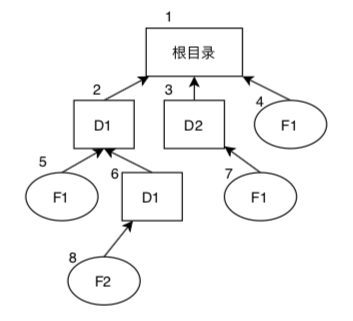
\includegraphics[width=0.5\textwidth]{image/21/3-p-1.png}
\end{figure}

如图所示,该图中绘制的文件系统共有 8 个文件。其中,方形表示目录文件,圆形表示普通文件,它们之间
的箭头表示含于关系。在表示文件的形状上的文字是其文件名;各个形状的左上方标记了序号,以便叙述。
在该文件系统中,文件 5 含于文件 2,文件 5 是文件 2 的孩子文件,文件 5 也是文件 2 的后代文件。
文件 8 是文件 2 的后代文件,但不是文件 2 的孩子文件。文件 8 的路径是 \verb|/D1/D1/F2|。

\subsubsection*{配额概述}
配额是指对文件系统中所含普通文件的总大小的限制。
对于每个目录 $d$,都可以设定两个配额值:{\heiti{目录配额}}和
{\heiti{后代配额}}。我们称目录配额 $LD_{d}$ 是{\heiti{满足的}},当且仅当 $d$ 的孩子文件中,
全部普通文件占用的存储空间之和不大于该配额值。我们称后代配额 $LR_{d}$
是{\heiti{满足的}},当且仅当 $d$ 的后代文件中,全部普通文件占用的存储空间之和不大于该配额值。
我们称文件系统的配额是满足的,当且仅当该文件系统中所有的配额都是满足的。

很显然,若文件系统中仅存在目录,不存在普通文件,那么该文件系统的配额一定是满足的。随着配额和文件
的创建,某个操作会使文件系统的配额由满足变为不满足,这样的操作会被拒绝。例如:试图设定少于目前已有
文件占用空间的配额值,或者试图创建超过配额值的文件。

\subsection*{题目描述}

在本题中,假定初始状态下,文件系统仅包含根目录。你将会收到若干对文件系统的操作指令。对于每条指令,
你需要判断该指令能否执行成功,对于能执行成功的指令,在成功执行该指令后,文件系统将会被相应地修改。
对于不能执行成功的指令,文件系统将{\heiti{不会发生任何变化}}。你需要处理的指令如下:

\subsubsection*{创建普通文件}

创建普通文件指令的格式如下:

\begin{lstlisting}
C <file path> <file size>
\end{lstlisting}

创建普通文件的指令有两个参数,是空格分隔的字符串和一个正整数,分别表示需要创建的普通文件的路径和
文件的大小。

对于该指令,若路径所指的文件已经存在,且也是普通文件的,
则替换这个文件;若路径所指文件已经存在,但是目录文件的,则该指令不能执行成功。

当路径中的任何目录不存在时,应当尝试创建这些目录;若要创建的目录文件与已有的同一双亲目录下的孩子
文件中的普通文件名称重复,则该指令不能执行成功。

另外,还需要确定在该指令的执行是否会使该文件系统的
配额变为不满足,如果会发生这样的情况,则认为该指令不能执行成功,反之则认为该指令能执行成功。

\subsubsection*{移除文件}

移除文件指令的格式如下:

\begin{lstlisting}
R <file path>
\end{lstlisting}

移除文件的指令有一个参数,是字符串,表示要移除的文件的路径。

若该路径所指的文件不存在,则不进行任何操作。

若该路径所指的文件是目录,则移除该目录及其所有后代文件。

在上述过程中被移除的目录(如果有)上设置的配额值也被移除。

该指令始终认为能执行成功。

\subsubsection*{设置配额值}

\begin{lstlisting}
Q <file path> <LD> <LR>
\end{lstlisting}

设置配额值的指令有三个参数,是空格分隔的字符串和两个非负整数,分别表示需要设置配额值的目录
的路径、目录配额和后代配额。

该指令表示对所指的目录文件,
分别设置目录配额和后代配额。若路径所指的文件不存在,或者不是目录文件,则
该指令执行不成功。

若在该目录上已经设置了配额,则将原配额值替换为指定的配额值。

特别地,若配额值为 0,
则表示不对该项配额进行限制。若在应用新的配额值后,该文件系统配额变为不满足,那么该指令执行不成功。


\subsection*{输入格式}

从标准输入读入数据。

输入的第一行包含一个正整数 $n$,表示需要处理的指令条数。

输入接下来会有 $n$ 行,每一行一个指令。指令的格式符合前述要求。输入数据保证:对于所有指令,
输入的路径是合法路径;对于创建普通文件和移除文件指令,输入的路径不指向根目录。


\subsection*{输出格式}

输出到标准输出。

输出共有 $n$ 行,表示相应的操作指令是否执行成功。若成功执行,则输出字母 \verb|Y|;否则输出 \verb|N|。

\examplebox*{\lstinputlisting[frame=none]{data/21/3-1.in}}{\lstinputlisting[frame=none]{data/21/3-1.out}}

输入总共有 10 条指令。其中前两条指令可以正常创建两个普通文件。第三条指令试图创建 /A/B/1/3,
但是 /A/B/1 已经存在,且不是目录,而是普通文件,不能再进一步创建孩子文件,因此执行不成功。
第四条指令试图创建 /A,但是 /A 已经存在,且是目录,因此执行不成功。第五条指令试图删除 /A/B/1/3,
由于该文件不存在,因此不对文件系统进行修改,但是仍然认为执行成功。第六条指令试图在根目录
增加后代配额限制,但此时,文件系统中的文件总大小是 2048,因此该限制无法生效,执行不成功。
第七条指令试图创建文件 /A/B/1,由于 /A/B/1 已经存在,且是普通文件,因此该指令实际效果是
将原有的该文件替换。此时文件总大小是 1124,因此第八条指令就可以执行成功了。
第九条指令递归删除了 /A/B 目录和它的所有后代文件。此时文件系统中已经没有普通文件,因此第十条命令
可以执行成功。

\examplebox*{\lstinputlisting[frame=none]{data/21/3-2.in}}{\lstinputlisting[frame=none]{data/21/3-2.out}}

输入共有 9 条指令。第一条指令试图为 /A/B 创建配额规则,然而该目录并不存在,因此执行不成功。
接下来的两条指令创建了两个普通文件。再接下来的两条指令分别在目录 /A/B 和 /A/C 创建了
两个配额规则。其中前者是目录配额,后者是后代配额。接下来的两条指令,创建了
两个文件。其中,/A/B/3 超出了在 /A/B 的目录配额,因此执行不成功;但 /A/B/D/3
不受目录配额限制,因此执行成功。最后两条指令,创建了两个文件。虽然在 /A/C
没有目录配额限制,但是无论是 /A/C 下的孩子文件还是后代文件,都受到后代配额的限制,因此两条指令
执行都不成功。

\subsection*{子任务}

本题目各个测试点的数据规模如下:

\begin{table}[H]
    \centering
    \begin{tabular}{c|c|c|c|c|c}
        % \toprule
        \thickhline
        测试点   & 操作数                      & 单个文件大小                & 路径长度                   & 目录层次                  & 没有操作 $Q$ \\ \hline
        % \midrule
        $1,2$    & \multirow{2}{*}{$\le 100$}  & \multirow{4}{*}{$\le 10^9$} & \multirow{4}{*}{$\le 100$} & \multirow{4}{*}{$\le 20$} & 是           \\ \cline{1-1} \cline{6-6}
        $3,4$    &                             &                             &                            &                           & 否           \\ \cline{1-2} \cline{6-6}
        $5,6,7$  & \multirow{2}{*}{$\le 10^5$} &                             &                            &                           & 是           \\ \cline{1-1} \cline{6-6}
        $8,9,10$ &                             &                             &                            &                           & 否           \\ \thickhline
        % \bottomrule
    \end{tabular}
\end{table}

表格中,目录层次是指各指令中出现的路径中,\verb|/| 字符的数目。

所有输入的数字均不超过$10^{18}$。




% % \section{202012-4}

% \subsection*{题目背景}

在T市有很多个酒店,这些酒店对于不同种类的食材有不同的需求情况,莱莱公司负责每天给这些酒店运输食材。

由于酒店众多,如何规划运输路线成为了一个非常重要的问题。你作为莱莱公司的顾问,请帮他们解决这个棘手的问题。


\subsection*{题目描述}

T市有 $N$ 个酒店,这些酒店由 $N-1$ 条双向道路连接,所有酒店和道路构成一颗树。不同的道路可能有不同的长度,运输车通过该道路所需要的时间受道路的长度影响。

在T市,一共有 $K$ 种主流食材。莱莱公司有 $K$ 辆车,每辆车负责一种食材的配送,不存在多辆车配送相同的食材。

由于不同酒店的特点不同,因此不同酒店对食材的需求情况也不同,比如可能 $1$ 号酒店只需要第 $1,5$ 种食材, $2$ 号酒店需要全部的 $K$ 种食材。

莱莱公司每天给这些公司运输食材。对于运输第 $i$ 种食材的车辆,这辆车可以从任意酒店出发,然后将食材运输到所有需要第 $i$ 种食材的酒店。假设运输过程中食材的装卸不花时间,运输车足够大使得其能够在出发时就装满全部所需食材,并且食材的重量不影响运输车的速度。

为了提高配送效率,这 $K$ 辆车可以从不同的酒店出发。但是由于T市对于食品安全特别重视,因此每辆车在配送之前需要进行食品安全检查。鉴于进行食品安全检查的人手不足,最多可以设置 $M$ 个检查点。

现在莱莱公司需要你制定一个运输方案:选定{\heiti{不超过}} $M$ 个酒店设立食品安全检查点,确定每辆运输车从哪个检查点出发,规划每辆运输车的路线。

假设所有的食材运输车在进行了食品安全检查之后同时出发,请制定一个运输方案,使得所有酒店的等待时间的最大值最小。酒店的等待时间从运输车辆出发时开始计算,到该酒店所有需要的食材都运输完毕截至。如果一个酒店不需要任何食材,那么它的等待时间为 $0$ 。


\subsection*{输入格式}

从标准输入读入数据。

输入的第一行包含 $3$ 个正整数 $N,M,K$ ($1 \le N \le 10^{2}, 1 \le M \le K \le 10$),含义见题目描述。

接下来 $N$ 行,每行包含 $K$ 个整数。每行输入描述对应酒店对每种食材的需求情况, $1$ 表示需要对应的食材, $0$ 表示不需要。

接下来 $N-1$ 行,每行包含 $3$ 个整数 $u, v, w$ ,表示存在一条通行时间为 $w$ 的双向道路连接 $u$ 号酒店和 $v$ 号酒店。保证输入数据是一颗树,酒店从 $1$ 编号到 $N$ ,保证 $1 \le u,v \le N$ 并且 $1 \le w \le 10^{6}$。


\subsection*{输出格式}

输出到标准输出。

输出一个整数,表示在你的方案中,所有酒店的等待时间的最大值。

\examplebox*{\lstinputlisting[frame=none]{data/21/4-1.in}}{\lstinputlisting[frame=none]{data/21/4-1.out}}

\begin{figure}[H]
    \centering
    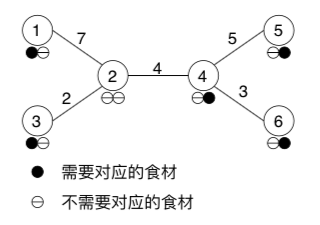
\includegraphics[width=0.6\textwidth]{image/21/4-p-1.png}
\end{figure}

样例1的输入数据如上图。由于限制了最多只能设置 $1$ 个检查点,因此可以设置两辆运输车的路径如下:

\begin{figure}[H]
    \centering
    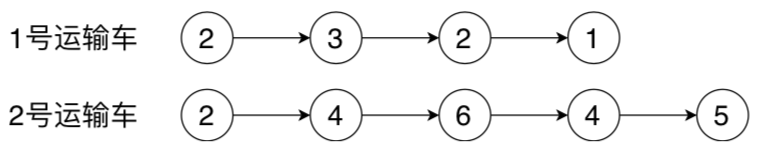
\includegraphics[width=0.9\textwidth]{image/21/4-p-2.png}
\end{figure}

在 $2$ 号酒店设置检查点,最晚拿到所有食材的酒店为 $3$ 号酒店,等待时间为 $9$。

\examplebox*{\lstinputlisting[frame=none]{data/21/4-2.in}}{\lstinputlisting[frame=none]{data/21/4-2.out}}

样例2的输入数据和样例1几乎完全相同,唯一的区别在于样例2中允许最多设置 $2$ 个检查点。我们可以设置两辆运输车的路径如下:

\begin{figure}[H]
    \centering
    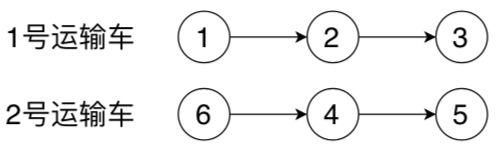
\includegraphics[width=0.9\textwidth]{image/21/4-p-3.png}
\end{figure}

在 $1$ 号酒店和 $6$ 号酒店设置检查点,最晚拿到所有食材的酒店为 $5$ 号酒店,等待时间为 $15$。

\subsection*{子任务}

本题目数据规模如下:

\begin{table}[H]
    \centering
    \begin{tabular}{c|c|c|c|c}
        \thickhline
        分数占比 & $N$                         & $M$                   & $K$                       & 特殊性                           \\ \hline
        $30\%$   & \multirow{3}{*}{$\le 10^2$} & \multirow{2}{*}{$=K$} & \multirow{3}{*}{$\le 10$} & 保证输入数据是一条链,且 $u+1=v$ \\ \cline{1-1} \cline{5-5}
        $40\%$   &                             &                       &                           & \multirow{2}{*}{无}              \\ \cline{1-1} \cline{3-3}
        $30\%$   &                             & $\le k$               &                           &                                  \\ \thickhline
    \end{tabular}
\end{table}

% % \section{202012-5}

% \subsection*{题目描述}

乔帝要规划一次星际旅行,星际空间可以视为一个 $3$ 维坐标系,乔帝有 $n(n\leq1,000,000,000)$ 个动力装置排成一行(下标从 $1$ 到 $n$ )。

第 $i$ 个动力装置可以让他的飞船 $3$ 个维度的坐标分别增加 $x_i,y_i,z_i$ 。一开始这些动力装置的所有参数都是 $0$ 。

在规划过程中,乔帝可能会对动力装置进行调整,也可能会对一些动力装置的动力进行评估。

具体来说,乔帝会进行 $m(m\leq40000)$ 次操作,每次操作可能是以下四种操作之一:

\begin{itemize}

    \item 动力增加:指定一个区间 $[L,R]$ 和三个参数 $a,b,c$ ,令区间内所有动力装置的3维坐标分别增加 $a,b,c$



    \item 动力强化:指定一个区间 $[L,R]$ 和一个参数 $k$ ,令区间内所有动力装置的3维坐标分别乘 $k$



    \item 动力转向:指定一个区间 $[L,R]$ ,令区间内所有动力装置的 $x,y,z$ 坐标分别变为原来的 $y$ 坐标, $z$ 坐标,$x$ 坐标



    \item 动力查询:指定一个区间 $[L,R]$ ,询问如果使用区间内所有动力装置各一次能将乔帝送到离起点多远的地方(输出距离的平方除以1,000,000,007的余数)



\end{itemize}


\subsection*{输入格式}

从标准输入读入数据。

第一行包含两个正整数 $n,m$。

接下来 $m$ 行,每行用若干个空格分隔的整数表示一个操作。

每行的第一个整数表示这次进行的是哪一种操作,$1,2,3,4$分别表示动力增加、动力强化、动力转向、动力查询。

每行的接下来两个整数表示 $L,R$,含义如上面所述。

每行接下来若干个整数,根据操作类型确定,为$a,b,c$或$k$或空。


\subsection*{输出格式}

输出到标准输出。

对于每个动力查询操作,输出一行,包含一个整数,表示查询的答案。

\examplebox*{\lstinputlisting[frame=none]{data/21/5-1.in}}{\lstinputlisting[frame=none]{data/21/5-1.out}}

一共有 $5$ 个动力装置。

对于第 $1$ 个操作,令第 $2,3,4$ 个动力装置的动力变为 $(5,6,7)$。

对于第 $2$ 个操作,令第 $5$ 个动力装置转向,为 $(0,0,0)$。

对于第 $3$ 个操作,令第 $1,2$ 个动力装置变为原来的 $4$ 倍,第一个变为 $(0,0,0)$ ,第二个变为 $(20,24,28)$。

对于第 $4$ 个操作,是查询,送到离起点 $(0+20+5,0+24+6,0+28+7)$,距离的平方为 $2750$。

对于第 $5$ 个操作,也是查询,送到离起点 $(20+5+5+0,24+6+6+0,28+7+7+0)$,距离的平方为 $3960$。

\subsection*{子任务}

对于 $20\%$ 的数据,$n,m\leq 1000$;

对于另外 $20\%$ 的数据,$n\leq 100000$,且只包含第$1,4$种操作;

对于另外 $20\%$ 的数据,$n\leq 100000$,且只包含第$1,2,4$种操作;

对于另外 $20\%$ 的数据,$n\leq 100000$;

对于另外 $20\%$ 的数据,没有特殊性质。

所有输入的数字都在 $[1,1000000000]$范围内。

所有的数据中 $1\leq m\leq 40000$。

所有的操作满足 $1\leq L\leq R\leq n$。


% 第22次认证(2021年04月)

\chapter{第22次认证(2021年04月)}

\section{题目及设计知识点}

\begin{table}[htbp]
  \centering
  \begin{tabular}{ccc}
    \toprule
    题目编号 & 题目名称   & 知识点 \\
    \midrule
    1        & 灰度直方图 &        \\
    2        & 邻域均值   &        \\
    3        & DHCP服务器 &        \\
    4        & 校门外的树 &        \\
    5        & 疫苗运输   &        \\
    \bottomrule
  \end{tabular}
\end{table}

\newpage
\section{202104-1 灰度直方图}
\ifonlyanalyze
\else
  \subsection*{题目描述}

一幅长宽分别为 $n$ 个像素和 $m$ 个像素的灰度图像可以表示为一个 $n \times m$ 大小的矩阵 $A$。

其中每个元素 $A_{ij}$($0 \le i <n$、$0 \le j < m$)是一个 $[0, L)$ 范围内的整数,表示对应位置像素的灰度值。

具体来说,一个 $8$ 比特的灰度图像中每个像素的灰度范围是 $[0, 128)$。

一副灰度图像的灰度统计直方图(以下简称“直方图”)可以表示为一个长度为 $L$ 的数组 $h$,其中 $h[x]$($0 \le x < L$)表示该图像中灰度值为 $x$ 的像素个数。显然,$h[0]$ 到 $h[L-1]$ 的总和应等于图像中的像素总数 $n \cdot m$。

已知一副图像的灰度矩阵 $A$,试计算其灰度直方图 $h[0], h[1], \cdots, h[L-1]$。


\subsection*{输入格式}

输入共 $n + 1$ 行。

输入的第一行包含三个用空格分隔的正整数 $n$、$m$ 和 $L$,含义如前文所述。

第二到第 $n + 1$ 行输入矩阵 $A$。

第 $i + 2$($0 \le i < n$)行包含用空格分隔的 $m$ 个整数,依次为 $A_{i0}, A_{i1}, \cdots, A_{i(m-1)}$。


\subsection*{输出格式}

输出仅一行,包含用空格分隔的 $L$ 个整数 $h[0], h[1], \cdots, h[L-1]$,表示输入图像的灰度直方图。


\subsection*{样例}

输入\#1:

\begin{lstlisting}
4 4 16
0 1 2 3
4 5 6 7
8 9 10 11
12 13 14 15
\end{lstlisting}

输出\#1:

\begin{lstlisting}
1 1 1 1 1 1 1 1 1 1 1 1 1 1 1 1
\end{lstlisting}

输入\#2:

\begin{lstlisting}
7 11 8
0 7 0 0 0 7 0 0 7 7 0
7 0 7 0 7 0 7 0 7 0 7
7 0 0 0 7 0 0 0 7 0 7
7 0 0 0 0 7 0 0 7 7 0
7 0 0 0 0 0 7 0 7 0 0
7 0 7 0 7 0 7 0 7 0 0
0 7 0 0 0 7 0 0 7 0 0
\end{lstlisting}

输出\#2:

\begin{lstlisting}
48 0 0 0 0 0 0 29
\end{lstlisting}

\subsection*{子任务}

全部的测试数据满足 $0 < n, m \le 500$ 且 $4 \le L \le 256$。



\fi
% \section{202104-1}

% \subsection*{题目描述}

一幅长宽分别为 $n$ 个像素和 $m$ 个像素的灰度图像可以表示为一个 $n \times m$ 大小的矩阵 $A$。

其中每个元素 $A_{ij}$($0 \le i <n$、$0 \le j < m$)是一个 $[0, L)$ 范围内的整数,表示对应位置像素的灰度值。

具体来说,一个 $8$ 比特的灰度图像中每个像素的灰度范围是 $[0, 128)$。

一副灰度图像的灰度统计直方图(以下简称“直方图”)可以表示为一个长度为 $L$ 的数组 $h$,其中 $h[x]$($0 \le x < L$)表示该图像中灰度值为 $x$ 的像素个数。显然,$h[0]$ 到 $h[L-1]$ 的总和应等于图像中的像素总数 $n \cdot m$。

已知一副图像的灰度矩阵 $A$,试计算其灰度直方图 $h[0], h[1], \cdots, h[L-1]$。


\subsection*{输入格式}

输入共 $n + 1$ 行。

输入的第一行包含三个用空格分隔的正整数 $n$、$m$ 和 $L$,含义如前文所述。

第二到第 $n + 1$ 行输入矩阵 $A$。

第 $i + 2$($0 \le i < n$)行包含用空格分隔的 $m$ 个整数,依次为 $A_{i0}, A_{i1}, \cdots, A_{i(m-1)}$。


\subsection*{输出格式}

输出仅一行,包含用空格分隔的 $L$ 个整数 $h[0], h[1], \cdots, h[L-1]$,表示输入图像的灰度直方图。


\subsection*{样例}

输入\#1:

\begin{lstlisting}
4 4 16
0 1 2 3
4 5 6 7
8 9 10 11
12 13 14 15
\end{lstlisting}

输出\#1:

\begin{lstlisting}
1 1 1 1 1 1 1 1 1 1 1 1 1 1 1 1
\end{lstlisting}

输入\#2:

\begin{lstlisting}
7 11 8
0 7 0 0 0 7 0 0 7 7 0
7 0 7 0 7 0 7 0 7 0 7
7 0 0 0 7 0 0 0 7 0 7
7 0 0 0 0 7 0 0 7 7 0
7 0 0 0 0 0 7 0 7 0 0
7 0 7 0 7 0 7 0 7 0 0
0 7 0 0 0 7 0 0 7 0 0
\end{lstlisting}

输出\#2:

\begin{lstlisting}
48 0 0 0 0 0 0 29
\end{lstlisting}

\subsection*{子任务}

全部的测试数据满足 $0 < n, m \le 500$ 且 $4 \le L \le 256$。




\newpage
\section{202104-2 邻域均值}
\ifonlyanalyze
\else
  \subsection*{试题背景}

顿顿在学习了数字图像处理后,想要对手上的一副灰度图像进行降噪处理。不过该图像仅在较暗区域有很多噪点,如果贸然对全图进行降噪,会在抹去噪点的同时也模糊了原有图像。因此顿顿打算先使用{\heiti{邻域均值}}来判断一个像素是否处于{\heiti{较暗区域}},然后仅对处于{\heiti{较暗区域}}的像素进行降噪处理。


\subsection*{问题描述}

待处理的灰度图像长宽皆为 $n$ 个像素,可以表示为一个 $n \times n$ 大小的矩阵 $A$,其中每个元素是一个 $[0, L)$ 范围内的整数,表示对应位置像素的灰度值。
对于矩阵中任意一个元素 $A_{ij}$($0 \le i, j < n$),其{\heiti{邻域}}定义为附近若干元素的集和:

\begin{equation*}
 Neighbor(i, j, r) = \left\{ A_{xy} | 0 \le x, y < n \mathrm{~and~} |x-i| \le r \mathrm{~and~} |y-j| \le r \right\} 
\end{equation*}


这里使用了一个额外的参数 $r$ 来指明 $A_{ij}$ 附近元素的具体范围。根据定义,易知 $Neighbor(i, j, r)$ 最多有 $(2r+1)^2$ 个元素。

如果元素 $A_{ij}$ {\heiti{邻域}}中所有元素的{\heiti{平均值}}小于或等于一个给定的阈值 $t$,我们就认为该元素对应位置的像素处于{\heiti{较暗区域}}。
下图给出了两个例子,左侧图像的较暗区域在右侧图像中展示为黑色,其余区域展示为白色。

% <img alt="example.jpg" src="/RequireFile.do?fid=9GqFey2d"/>
\begin{figure}[H]
    \centering
    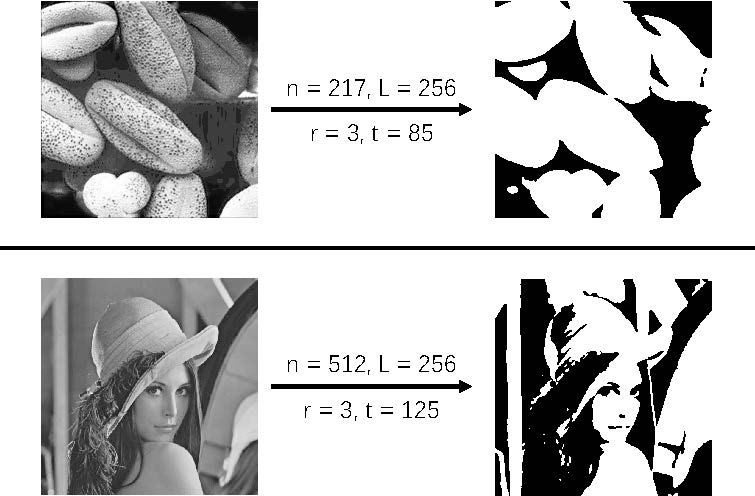
\includegraphics[width=0.95\textwidth]{image/22/2-p-1.jpg}
    % \caption{神经元 $v$ 变量随时间变化的曲线}
\end{figure}

现给定邻域参数 $r$ 和阈值 $t$,试统计输入灰度图像中有多少像素处于{\heiti{较暗区域}}。


\subsection*{输入格式}

输入共 $n + 1$ 行。

输入的第一行包含四个用空格分隔的正整数 $n$、$L$、$r$ 和 $t$,含义如前文所述。

第二到第 $n + 1$ 行输入矩阵 $A$。
第 $i + 2$($0 \le i < n$)行包含用空格分隔的 $n$ 个整数,依次为 $A_{i0}, A_{i1}, \cdots, A_{i(n-1)}$。


\subsection*{输出格式}

输出一个整数,表示输入灰度图像中处于较暗区域的像素总数。

\subsection*{样例}

输入\#1:

\begin{lstlisting}
4 16 1 6
0 1 2 3
4 5 6 7
8 9 10 11
12 13 14 15
\end{lstlisting}

输出\#1:

\begin{lstlisting}
7
\end{lstlisting}

输入\#2:

\begin{lstlisting}
11 8 2 2
0 0 0 0 0 0 0 0 0 0 0
0 0 0 0 0 0 0 0 0 0 0
0 7 0 0 0 7 0 0 7 7 0
7 0 7 0 7 0 7 0 7 0 7
7 0 0 0 7 0 0 0 7 0 7
7 0 0 0 0 7 0 0 7 7 0
7 0 0 0 0 0 7 0 7 0 0
7 0 7 0 7 0 7 0 7 0 0
0 7 0 0 0 7 0 0 7 0 0
0 0 0 0 0 0 0 0 0 0 0
0 0 0 0 0 0 0 0 0 0 0
\end{lstlisting}

输出\#2:

\begin{lstlisting}
83
\end{lstlisting}

\subsection*{子任务}

$70\%$ 的测试数据满足 $n \le 100$、$r \le 10$。

全部的测试数据满足 $0 < n \le 600$、$0 < r \le 100$ 且 $2 \le t < L \le 256$。

\fi
% \section{202104-2}

% \subsection*{试题背景}

顿顿在学习了数字图像处理后,想要对手上的一副灰度图像进行降噪处理。不过该图像仅在较暗区域有很多噪点,如果贸然对全图进行降噪,会在抹去噪点的同时也模糊了原有图像。因此顿顿打算先使用{\heiti{邻域均值}}来判断一个像素是否处于{\heiti{较暗区域}},然后仅对处于{\heiti{较暗区域}}的像素进行降噪处理。


\subsection*{问题描述}

待处理的灰度图像长宽皆为 $n$ 个像素,可以表示为一个 $n \times n$ 大小的矩阵 $A$,其中每个元素是一个 $[0, L)$ 范围内的整数,表示对应位置像素的灰度值。
对于矩阵中任意一个元素 $A_{ij}$($0 \le i, j < n$),其{\heiti{邻域}}定义为附近若干元素的集和:

\begin{equation*}
 Neighbor(i, j, r) = \left\{ A_{xy} | 0 \le x, y < n \mathrm{~and~} |x-i| \le r \mathrm{~and~} |y-j| \le r \right\} 
\end{equation*}


这里使用了一个额外的参数 $r$ 来指明 $A_{ij}$ 附近元素的具体范围。根据定义,易知 $Neighbor(i, j, r)$ 最多有 $(2r+1)^2$ 个元素。

如果元素 $A_{ij}$ {\heiti{邻域}}中所有元素的{\heiti{平均值}}小于或等于一个给定的阈值 $t$,我们就认为该元素对应位置的像素处于{\heiti{较暗区域}}。
下图给出了两个例子,左侧图像的较暗区域在右侧图像中展示为黑色,其余区域展示为白色。

% <img alt="example.jpg" src="/RequireFile.do?fid=9GqFey2d"/>
\begin{figure}[H]
    \centering
    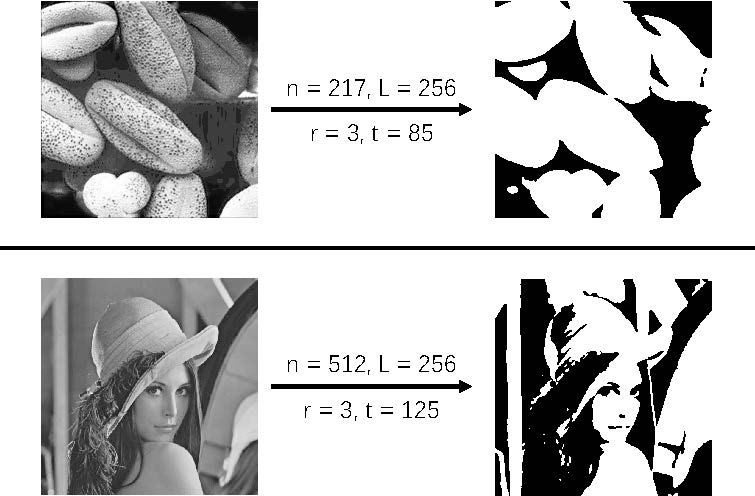
\includegraphics[width=0.95\textwidth]{image/22/2-p-1.jpg}
    % \caption{神经元 $v$ 变量随时间变化的曲线}
\end{figure}

现给定邻域参数 $r$ 和阈值 $t$,试统计输入灰度图像中有多少像素处于{\heiti{较暗区域}}。


\subsection*{输入格式}

输入共 $n + 1$ 行。

输入的第一行包含四个用空格分隔的正整数 $n$、$L$、$r$ 和 $t$,含义如前文所述。

第二到第 $n + 1$ 行输入矩阵 $A$。
第 $i + 2$($0 \le i < n$)行包含用空格分隔的 $n$ 个整数,依次为 $A_{i0}, A_{i1}, \cdots, A_{i(n-1)}$。


\subsection*{输出格式}

输出一个整数,表示输入灰度图像中处于较暗区域的像素总数。

\subsection*{样例}

输入\#1:

\begin{lstlisting}
4 16 1 6
0 1 2 3
4 5 6 7
8 9 10 11
12 13 14 15
\end{lstlisting}

输出\#1:

\begin{lstlisting}
7
\end{lstlisting}

输入\#2:

\begin{lstlisting}
11 8 2 2
0 0 0 0 0 0 0 0 0 0 0
0 0 0 0 0 0 0 0 0 0 0
0 7 0 0 0 7 0 0 7 7 0
7 0 7 0 7 0 7 0 7 0 7
7 0 0 0 7 0 0 0 7 0 7
7 0 0 0 0 7 0 0 7 7 0
7 0 0 0 0 0 7 0 7 0 0
7 0 7 0 7 0 7 0 7 0 0
0 7 0 0 0 7 0 0 7 0 0
0 0 0 0 0 0 0 0 0 0 0
0 0 0 0 0 0 0 0 0 0 0
\end{lstlisting}

输出\#2:

\begin{lstlisting}
83
\end{lstlisting}

\subsection*{子任务}

$70\%$ 的测试数据满足 $n \le 100$、$r \le 10$。

全部的测试数据满足 $0 < n \le 600$、$0 < r \le 100$ 且 $2 \le t < L \le 256$。


\newpage
\section{202104-3 DHCP服务器}
\ifonlyanalyze
\else
  \subsection*{试题背景}

{\heiti{动态主机配置协议}}(Dynamic Host Configuration Protocol, DHCP)是一种自动为网络客户端分配 IP 地址的网络协议。当支持该协议的计算机刚刚接入网络时,它可以启动一个 DHCP 客户端程序。后者可以通过一定的网络报文交互,从 DHCP 服务器上获得 IP 地址等网络配置参数,从而能够在用户不干预的情况下,自动完成对计算机的网络设置,方便用户连接网络。DHCP 协议的工作过程如下:

\begin{enumerate}

\item 当 DHCP 协议启动的时候,DHCP 客户端向网络中广播发送 Discover 报文,请求 IP 地址配置;

\item 当 DHCP 服务器收到 Discover 报文时,DHCP 服务器根据报文中的参数选择一个尚未分配的 IP 地址,分配给该客户端。DHCP 服务器用 Offer 报文将这个信息传达给客户端;

\item 客户端收集收到的 Offer 报文。由于网络中可能存在多于一个 DHCP 服务器,因此客户端可能收集到多个 Offer 报文。客户端从这些报文中选择一个,并向网络中广播 Request 报文,表示选择这个 DHCP 服务器发送的配置;

\item DHCP 服务器收到 Request 报文后,首先判断该客户端是否选择本服务器分配的地址:如果不是,则在本服务器上解除对那个 IP 地址的占用;否则则再次确认分配的地址有效,并向客户端发送 Ack 报文,表示确认配置有效,Ack 报文中包括配置的有效时间。如果 DHCP 发现分配的地址无效,则返回 Nak 报文;

\item 客户端收到 Ack 报文后,确认服务器分配的地址有效,即确认服务器分配的地址未被其它客户端占用,则完成网络配置,同时记录配置的有效时间,出于简化的目的,我们不考虑被占用的情况。若客户端收到 Nak 报文,则从步骤 1 重新开始;

\item 客户端在到达配置的有效时间前,再次向 DHCP 服务器发送 Request 报文,表示希望延长 IP 地址的有效期。DHCP 服务器按照步骤 4 确定是否延长,客户端按照步骤 5 处理后续的配置;

\end{enumerate}

在本题目中,你需要理解 DHCP 协议的工作过程,并按照题目的要求实现一个简单的 DHCP 服务器。


\subsection*{问题描述}

\subsubsection*{报文格式}

为了便于实现,我们简化地规定 DHCP 数据报文的格式如下:

\begin{lstlisting}
<发送主机> <接收主机> <报文类型> <IP 地址> <过期时刻>
\end{lstlisting}

DHCP 数据报文的各个部分由空格分隔,其各个部分的定义如下:

\begin{itemize}

\item 发送主机:是发送报文的主机名,{\heiti{主机名}}是由小写字母、数字组成的字符串,唯一地表示了一个主机;

\item 接收主机:当有特定的接收主机时,是接收报文的主机名;当没有特定的接收主机时,为一个星号(\verb|*|);

\item 报文类型:是三个大写字母,取值如下:\begin{itemize}

\item \verb|DIS|:表示 Discover 报文;

\item \verb|OFR|:表示 Offer 报文;

\item \verb|REQ|:表示 Request 报文;

\item \verb|ACK|:表示 Ack 报文;

\item \verb|NAK|:表示 Nak 报文;

\end{itemize}



\item IP 地址,是一个非负整数:\begin{itemize}

\item 对于 Discover 报文,该部分在发送的时候为 0,在接收的时候忽略;

\item 对于其它报文,为正整数,表示一个 IP 地址;

\end{itemize}



\item 过期时刻,是一个非负整数:\begin{itemize}

\item 对于 Offer、Ack 报文,是一个正整数,表示服务器授予客户端的 IP 地址的过期时刻;

\item 对于 Discover、Request 报文,若为正整数,表示客户端期望服务器授予的过期时刻;

\item 对于其它报文,该部分在发送的时候为 0,在接收的时候忽略。

\end{itemize}



\end{itemize}

例如下列都是合法的 DHCP 数据报文:

\begin{lstlisting}
a * DIS 0 0
d a ACK 50 1000
\end{lstlisting}

\subsubsection*{服务器配置}

为了 DHCP 服务器能够正确分配 IP 地址,DHCP 需要接受如下配置:

\begin{itemize}

\item 地址池大小 $N$:表示能够分配给客户端的 IP 地址的数目,且能分配的 IP 地址是 $1, 2, \dots, N$;

\item 默认过期时间 $T_{def}$:表示分配给客户端的 IP 地址的默认的过期时间长度;

\item 过期时间的上限和下限 $T_{max}$、$T_{min}$:表示分配给客户端的 IP 地址的最长过期时间长度和最短过期时间长度,客户端不能请求比这个更长或更短的过期时间;

\item 本机名称 $H$:表示运行 DHCP 服务器的主机名。

\end{itemize}

\subsubsection*{分配策略}

当客户端请求 IP 地址时,首先检查此前是否给该客户端分配过 IP 地址,且该 IP 地址在此后没有被分配给其它客户端。如果是这样的情况,则直接将 IP 地址分配给它,否则,
总是分配给它最小的尚未占用过的那个 IP 地址。如果这样的地址不存在,则分配给它最小的此时未被占用的那个 IP 地址。如果这样的地址也不存在,说明地址池已经分配完毕,因此拒绝分配地址。

\subsubsection*{实现细节}

在 DHCP 启动时,首先初始化 IP 地址池,将所有地址设置状态为未分配,占用者为空,并清零过期时刻。
其中地址的状态有未分配、待分配、占用、过期四种。
处于未分配状态的 IP 地址没有占用者,而其余三种状态的 IP 地址均有一名占用者。
处于待分配和占用状态的 IP 地址拥有一个大于零的过期时刻。在到达该过期时刻时,若该地址的状态是待分配,则该地址的状态会自动变为未分配,且占用者清空,过期时刻清零;否则该地址的状态会由占用自动变为过期,且过期时刻清零。处于未分配和过期状态的 IP 地址过期时刻为零,即没有过期时刻。

对于收到的报文,设其收到的时刻为 $t$。处理细节如下:

\begin{enumerate}

\item 判断接收主机是否为本机,或者为 \verb|*|,若不是,则判断类型是否为 Request,若不是,则不处理;

\item 若类型不是 Discover、Request 之一,则不处理;

\item 若接收主机为 \verb|*|,但类型不是 Discover,或接收主机是本机,但类型是 Discover,则不处理。

\end{enumerate}

对于 Discover 报文,按照下述方法处理:

\begin{enumerate}

\item 检查是否有占用者为发送主机的 IP 地址:\begin{itemize}

\item 若有,则选取该 IP 地址;

\item 若没有,则选取最小的状态为未分配的 IP 地址;

\item 若没有,则选取最小的状态为过期的 IP 地址;

\item 若没有,则不处理该报文,处理结束;

\end{itemize}



\item 将该 IP 地址状态设置为待分配,占用者设置为发送主机;

\item 若报文中过期时刻为 0 ,则设置过期时刻为 $t + T_{def}$;否则根据报文中的过期时刻和收到报文的时刻计算过期时间,判断是否超过上下限:若没有超过,则设置过期时刻为报文中的过期时刻;否则则根据超限情况设置为允许的最早或最晚的过期时刻;

\item 向发送主机发送 Offer 报文,其中,IP 地址为选定的 IP 地址,过期时刻为所设定的过期时刻。

\end{enumerate}

对于 Request 报文,按照下述方法处理:

\begin{enumerate}

\item 检查接收主机是否为本机:\begin{itemize}

\item 若不是,则找到占用者为发送主机的所有 IP 地址,对于其中状态为待分配的,将其状态设置为未分配,并清空其占用者,清零其过期时刻,处理结束;

\end{itemize}



\item 检查报文中的 IP 地址是否在地址池内,且其占用者为发送主机,若不是,则向发送主机发送 Nak 报文,处理结束;

\item 无论该 IP 地址的状态为何,将该 IP 地址的状态设置为占用;

\item 与 Discover 报文相同的方法,设置 IP 地址的过期时刻;

\item 向发送主机发送 Ack 报文。

\end{enumerate}

上述处理过程中,地址池中地址的状态的变化可以概括为如下图所示的状态转移图。为了简洁,该图中没有涵盖需要回复 Nak 报文的情况。

% <img alt="state_h.jpg" src="/RequireFile.do?fid=qUtXBjol"/>
\begin{figure}[H]
    \centering
    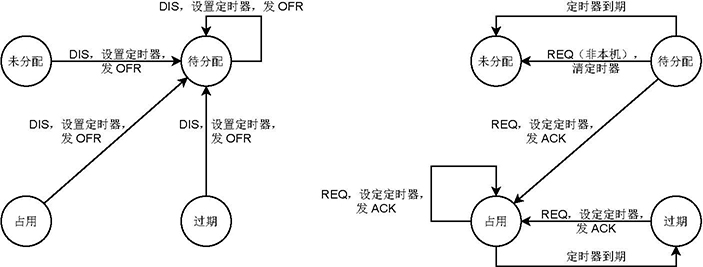
\includegraphics[width=0.95\textwidth]{image/22/3-p-1.jpg}
    % \caption{神经元 $v$ 变量随时间变化的曲线}
\end{figure}


\subsection*{输入格式}

输入的第一行包含用空格分隔的四个正整数和一个字符串,分别是:$N$、$T_{def}$、$T_{max}$、$T_{min}$ 和 $H$,保证 $T_{min} \le T_{def} \le T_{max}$。

输入的第二行是一个正整数 $n$,表示收到了 $n$ 个报文。

输入接下来有 $n$ 行,第 $(i+2)$ 行有空格分隔的正整数 $t_i$ 和约定格式的报文 $P_i$。表示收到的第 $i$ 个报文是在 $t_i$ 时刻收到的,报文内容是 $P_i$。保证 $t_i < t_{i+1}$。


\subsection*{输出格式}

输出有若干行,每行是一个约定格式的报文。依次输出 DHCP 服务器发送的报文。



\fi
% \section{202104-3}

% \subsection*{试题背景}

{\heiti{动态主机配置协议}}(Dynamic Host Configuration Protocol, DHCP)是一种自动为网络客户端分配 IP 地址的网络协议。当支持该协议的计算机刚刚接入网络时,它可以启动一个 DHCP 客户端程序。后者可以通过一定的网络报文交互,从 DHCP 服务器上获得 IP 地址等网络配置参数,从而能够在用户不干预的情况下,自动完成对计算机的网络设置,方便用户连接网络。DHCP 协议的工作过程如下:

\begin{enumerate}

\item 当 DHCP 协议启动的时候,DHCP 客户端向网络中广播发送 Discover 报文,请求 IP 地址配置;

\item 当 DHCP 服务器收到 Discover 报文时,DHCP 服务器根据报文中的参数选择一个尚未分配的 IP 地址,分配给该客户端。DHCP 服务器用 Offer 报文将这个信息传达给客户端;

\item 客户端收集收到的 Offer 报文。由于网络中可能存在多于一个 DHCP 服务器,因此客户端可能收集到多个 Offer 报文。客户端从这些报文中选择一个,并向网络中广播 Request 报文,表示选择这个 DHCP 服务器发送的配置;

\item DHCP 服务器收到 Request 报文后,首先判断该客户端是否选择本服务器分配的地址:如果不是,则在本服务器上解除对那个 IP 地址的占用;否则则再次确认分配的地址有效,并向客户端发送 Ack 报文,表示确认配置有效,Ack 报文中包括配置的有效时间。如果 DHCP 发现分配的地址无效,则返回 Nak 报文;

\item 客户端收到 Ack 报文后,确认服务器分配的地址有效,即确认服务器分配的地址未被其它客户端占用,则完成网络配置,同时记录配置的有效时间,出于简化的目的,我们不考虑被占用的情况。若客户端收到 Nak 报文,则从步骤 1 重新开始;

\item 客户端在到达配置的有效时间前,再次向 DHCP 服务器发送 Request 报文,表示希望延长 IP 地址的有效期。DHCP 服务器按照步骤 4 确定是否延长,客户端按照步骤 5 处理后续的配置;

\end{enumerate}

在本题目中,你需要理解 DHCP 协议的工作过程,并按照题目的要求实现一个简单的 DHCP 服务器。


\subsection*{问题描述}

\subsubsection*{报文格式}

为了便于实现,我们简化地规定 DHCP 数据报文的格式如下:

\begin{lstlisting}
<发送主机> <接收主机> <报文类型> <IP 地址> <过期时刻>
\end{lstlisting}

DHCP 数据报文的各个部分由空格分隔,其各个部分的定义如下:

\begin{itemize}

\item 发送主机:是发送报文的主机名,{\heiti{主机名}}是由小写字母、数字组成的字符串,唯一地表示了一个主机;

\item 接收主机:当有特定的接收主机时,是接收报文的主机名;当没有特定的接收主机时,为一个星号(\verb|*|);

\item 报文类型:是三个大写字母,取值如下:\begin{itemize}

\item \verb|DIS|:表示 Discover 报文;

\item \verb|OFR|:表示 Offer 报文;

\item \verb|REQ|:表示 Request 报文;

\item \verb|ACK|:表示 Ack 报文;

\item \verb|NAK|:表示 Nak 报文;

\end{itemize}



\item IP 地址,是一个非负整数:\begin{itemize}

\item 对于 Discover 报文,该部分在发送的时候为 0,在接收的时候忽略;

\item 对于其它报文,为正整数,表示一个 IP 地址;

\end{itemize}



\item 过期时刻,是一个非负整数:\begin{itemize}

\item 对于 Offer、Ack 报文,是一个正整数,表示服务器授予客户端的 IP 地址的过期时刻;

\item 对于 Discover、Request 报文,若为正整数,表示客户端期望服务器授予的过期时刻;

\item 对于其它报文,该部分在发送的时候为 0,在接收的时候忽略。

\end{itemize}



\end{itemize}

例如下列都是合法的 DHCP 数据报文:

\begin{lstlisting}
a * DIS 0 0
d a ACK 50 1000
\end{lstlisting}

\subsubsection*{服务器配置}

为了 DHCP 服务器能够正确分配 IP 地址,DHCP 需要接受如下配置:

\begin{itemize}

\item 地址池大小 $N$:表示能够分配给客户端的 IP 地址的数目,且能分配的 IP 地址是 $1, 2, \dots, N$;

\item 默认过期时间 $T_{def}$:表示分配给客户端的 IP 地址的默认的过期时间长度;

\item 过期时间的上限和下限 $T_{max}$、$T_{min}$:表示分配给客户端的 IP 地址的最长过期时间长度和最短过期时间长度,客户端不能请求比这个更长或更短的过期时间;

\item 本机名称 $H$:表示运行 DHCP 服务器的主机名。

\end{itemize}

\subsubsection*{分配策略}

当客户端请求 IP 地址时,首先检查此前是否给该客户端分配过 IP 地址,且该 IP 地址在此后没有被分配给其它客户端。如果是这样的情况,则直接将 IP 地址分配给它,否则,
总是分配给它最小的尚未占用过的那个 IP 地址。如果这样的地址不存在,则分配给它最小的此时未被占用的那个 IP 地址。如果这样的地址也不存在,说明地址池已经分配完毕,因此拒绝分配地址。

\subsubsection*{实现细节}

在 DHCP 启动时,首先初始化 IP 地址池,将所有地址设置状态为未分配,占用者为空,并清零过期时刻。
其中地址的状态有未分配、待分配、占用、过期四种。
处于未分配状态的 IP 地址没有占用者,而其余三种状态的 IP 地址均有一名占用者。
处于待分配和占用状态的 IP 地址拥有一个大于零的过期时刻。在到达该过期时刻时,若该地址的状态是待分配,则该地址的状态会自动变为未分配,且占用者清空,过期时刻清零;否则该地址的状态会由占用自动变为过期,且过期时刻清零。处于未分配和过期状态的 IP 地址过期时刻为零,即没有过期时刻。

对于收到的报文,设其收到的时刻为 $t$。处理细节如下:

\begin{enumerate}

\item 判断接收主机是否为本机,或者为 \verb|*|,若不是,则判断类型是否为 Request,若不是,则不处理;

\item 若类型不是 Discover、Request 之一,则不处理;

\item 若接收主机为 \verb|*|,但类型不是 Discover,或接收主机是本机,但类型是 Discover,则不处理。

\end{enumerate}

对于 Discover 报文,按照下述方法处理:

\begin{enumerate}

\item 检查是否有占用者为发送主机的 IP 地址:\begin{itemize}

\item 若有,则选取该 IP 地址;

\item 若没有,则选取最小的状态为未分配的 IP 地址;

\item 若没有,则选取最小的状态为过期的 IP 地址;

\item 若没有,则不处理该报文,处理结束;

\end{itemize}



\item 将该 IP 地址状态设置为待分配,占用者设置为发送主机;

\item 若报文中过期时刻为 0 ,则设置过期时刻为 $t + T_{def}$;否则根据报文中的过期时刻和收到报文的时刻计算过期时间,判断是否超过上下限:若没有超过,则设置过期时刻为报文中的过期时刻;否则则根据超限情况设置为允许的最早或最晚的过期时刻;

\item 向发送主机发送 Offer 报文,其中,IP 地址为选定的 IP 地址,过期时刻为所设定的过期时刻。

\end{enumerate}

对于 Request 报文,按照下述方法处理:

\begin{enumerate}

\item 检查接收主机是否为本机:\begin{itemize}

\item 若不是,则找到占用者为发送主机的所有 IP 地址,对于其中状态为待分配的,将其状态设置为未分配,并清空其占用者,清零其过期时刻,处理结束;

\end{itemize}



\item 检查报文中的 IP 地址是否在地址池内,且其占用者为发送主机,若不是,则向发送主机发送 Nak 报文,处理结束;

\item 无论该 IP 地址的状态为何,将该 IP 地址的状态设置为占用;

\item 与 Discover 报文相同的方法,设置 IP 地址的过期时刻;

\item 向发送主机发送 Ack 报文。

\end{enumerate}

上述处理过程中,地址池中地址的状态的变化可以概括为如下图所示的状态转移图。为了简洁,该图中没有涵盖需要回复 Nak 报文的情况。

% <img alt="state_h.jpg" src="/RequireFile.do?fid=qUtXBjol"/>
\begin{figure}[H]
    \centering
    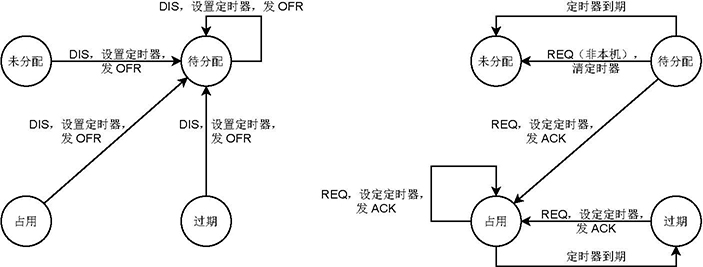
\includegraphics[width=0.95\textwidth]{image/22/3-p-1.jpg}
    % \caption{神经元 $v$ 变量随时间变化的曲线}
\end{figure}


\subsection*{输入格式}

输入的第一行包含用空格分隔的四个正整数和一个字符串,分别是:$N$、$T_{def}$、$T_{max}$、$T_{min}$ 和 $H$,保证 $T_{min} \le T_{def} \le T_{max}$。

输入的第二行是一个正整数 $n$,表示收到了 $n$ 个报文。

输入接下来有 $n$ 行,第 $(i+2)$ 行有空格分隔的正整数 $t_i$ 和约定格式的报文 $P_i$。表示收到的第 $i$ 个报文是在 $t_i$ 时刻收到的,报文内容是 $P_i$。保证 $t_i < t_{i+1}$。


\subsection*{输出格式}

输出有若干行,每行是一个约定格式的报文。依次输出 DHCP 服务器发送的报文。




\newpage
\section{202104-4 校门外的树}
\ifonlyanalyze
\else
  \subsection*{问题描述}

X 校最近打算美化一下校园环境。前段时间因为修地铁,X 校大门外种的行道树全部都被移走了。现在 X 校打算重新再种一些树,为校园增添一抹绿意。

X 校大门外的道路是东西走向的,我们可以将其看成一条数轴。在这条数轴上有 $n$ 个障碍物,例如电线杆之类的。虽然障碍物会影响树的生长,但是障碍物不一定能被随便移走,所以 X 校规定在障碍物的位置上{\heiti{不能}}种树。$n$ 个障碍物的坐标都是整数;如果规定向东为正方向,则 $n$ 个障碍物的坐标按照从西到东的顺序分别为 $a_1, a_2, \cdots, a_n$。X 校打算在 $\left[a_1, a_n\right]$ 之间种一些树,使得这些树看起来比较美观。

X 校希望,在一定范围内,树应该是等间隔的。更具体地说,如果把 $[a_1, a_n)$ 划分成一些区间 $\left[a_{p_1}, a_{p_2}\right),\cdots,\left[a_{p_{m-1}},a_{p_m}\right)$($1=p_1<p_2<\cdots<p_m=n$),那么每个区间 $\left[a_{p_i},a_{p_{i+1}}\right)$ 内需要至少种一棵树,且该区间内种的树的坐标连同区间端点 $a_{p_i}, a_{p_{i+1}}$ 应该构成一个等差数列。不同区间的公差,也就是树的间隔可以不相同。

例如,如果障碍物位于 $0, 2, 6$ 这三处,那么我们可以选择在 $[0, 2)$ 和 $[2, 6)$ 分别种树,也可以选择在 $[0, 6)$ 等间隔种树。如果是分别在 $[0, 2)$ 和 $[2, 6)$ 种树,由于每个区间内至少要种一棵树,坐标 $1$ 上必须种树;而 $[2, 6)$ 上的树可以按照 $1$ 的间隔种下,也可以按照 $2$ 的间隔种下。下图表示了这两种美观的种树方案,其中橙色的圆表示障碍物,绿色的圆表示需要在这个位置种树,箭头上的数字表示种下这棵树时对应的间隔为多少。

% <img alt="sample1_h.png" src="/RequireFile.do?fid=UXylvpoV"/>
\begin{figure}[H]
    \centering
    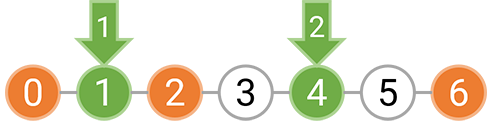
\includegraphics[width=0.95\textwidth]{image/22/4-p-1.png}
    % \caption{神经元 $v$ 变量随时间变化的曲线}
\end{figure}

对区间 $[0, 2)$ 和 $[2, 6)$ 分别以 $1$ 和 $2$ 的间隔种树是美观的

% <img alt="sample2_h.png" src="/RequireFile.do?fid=G97DdvfC"/>
\begin{figure}[H]
    \centering
    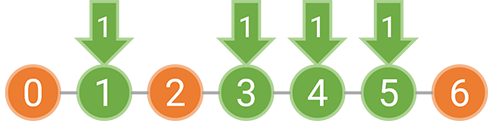
\includegraphics[width=0.95\textwidth]{image/22/4-p-2.png}
    % \caption{神经元 $v$ 变量随时间变化的曲线}
\end{figure}

对区间 $[0, 2)$ 和 $[2, 6)$ 分别以 $1$ 的间隔种树也是美观的

而如果选择在 $[0, 6)$ 区间等间隔种树,我们只能以 $3$ 的间隔种树,因为无论是选择间隔 $1$ 或者间隔 $2$,都需要在坐标 $2$ 上种树,而这个位置已经有障碍物了。下图分别表示了间隔为 $3, 2, 1$ 时的种树情况,红色箭头表示不能在这里种树。

% <img alt="sample3_h.png" src="/RequireFile.do?fid=dAQwSTuu"/>
\begin{figure}[H]
    \centering
    
\includegraphics[width=0.95\textwidth]{image/22/4-p-3.png}
    % \caption{神经元 $v$ 变量随时间变化的曲线}
\end{figure}

对区间 $[0, 6)$ 以 $3$ 的间隔种树是美观的

% <img alt="sample4_h.png" src="/RequireFile.do?fid=hpTkShxA"/>
\begin{figure}[H]
    \centering
    
\includegraphics[width=0.95\textwidth]{image/22/4-p-4.png}
    % \caption{神经元 $v$ 变量随时间变化的曲线}
\end{figure}

对区间 $[0, 6)$ 以 $2$ 的间隔种树是不美观的

% <img alt="sample5_h.png" src="/RequireFile.do?fid=oNrrpgBz"/>
\begin{figure}[H]
    \centering
    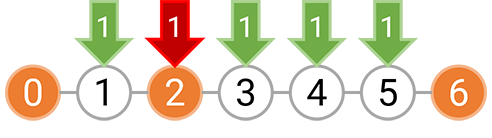
\includegraphics[width=0.95\textwidth]{image/22/4-p-5.png}
    % \caption{神经元 $v$ 变量随时间变化的曲线}
\end{figure}

对区间 $[0, 6)$ 以 $1$ 的间隔种树也是不美观的

一般地,给定一个区间 $[a_l, a_r)$,对于树的坐标的集合 $T\subset(a_l, a_r)$($T\subset\mathbb{Z}$),归纳定义 $T$ 在 $[a_l, a_r)$ 上是{\heiti{美观的}}:

\begin{enumerate}

    \item 如果 $T\ne \emptyset$,$T\cap \left\{a_l, a_{l+1}, \cdots, a_r\right\}=\emptyset$,并且存在一个公差 $d\ge 1$,使得 $T\cup\left\{a_l, a_r\right\}$ 中的元素按照从小到大的顺序排序后,可以构成一个公差为 $d$ 的等差数列(显然,这个等差数列的首项为 $a_l$,末项为 $a_r$),则 $T$ 在 $\left[a_l, a_r\right)$ 上是美观的;

    \item 如果 $T\cap \left\{a_l, a_{l+1}, \cdots, a_r\right\}=\emptyset$,并且存在一个下标 $m$($l<m<r$),使得 $T\cap\left(a_l, a_m\right)$ 在 $\left[a_l, a_m\right)$ 上是美观的,且 $T\cap\left(a_m, a_r\right)$ 在 $\left[a_m, a_r\right)$ 上是美观的,则 $T$ 在 $\left[a_l, a_r\right)$ 上是美观的。

\end{enumerate}

根据这一定义,空集在任意区间上都不是美观的;另外,如果存在下标 $i$ 使得 $a_i \in T$,那么 $T$ 一定不是美观的。

我们称两种种树的方案是{\heiti{本质不同的}},当且仅当两种方案中,种树的坐标集合不同。请帮助 X 校对 $\left[a_1, a_n\right)$ 求出所有本质不同的美观的种树方案。当然,由于方案可能很多,你只需要输出总方案数对 $10^9+7$ 取模的结果。


\subsection*{输入格式}

输入的第一行包含一个正整数 $n$,表示障碍物的数量。

输入的第二行包括 $n$ 个非负整数 $a_1, \cdots, a_n$,表示每个障碍物的坐标。

保证对 $i=1, 2, \cdots, n-1$,$a_i < a_{i+1}$。


\subsection*{输出格式}

输出一个非负整数,表示本质不同的美观的种树方案的数量对 $10^9+7$ 取模的结果。

\examplebox*{\lstinputlisting[frame=none]{data/22/4-1.in}}{\lstinputlisting[frame=none]{data/22/4-1.out}}

这组样例即为题面描述中提到的那组。

\examplebox{\lstinputlisting[frame=none]{data/22/4-2.in}}{\lstinputlisting[frame=none]{data/22/4-2.out}}

\examplebox{见 \href{data/22/4-3.in}{data/22/4-3.in}}{见 \href{data/22/4-3.out}{data/22/4-3.out}}

\subsection*{子任务}

对于 $10\%$ 的数据,保证 $n=2$;

对于 $30\%$ 的数据,保证 $n\le 10$;

对于 $60\%$ 的数据,保证 $n\le 100,a_i\le 1000$;

对于 $1000\%$ 的数据,保证 $2\le n\le 1000,0\le a_i\le 10^5$,且至少存在一种美观的种树方案。
\fi
% \section{202104-4}

% \subsection*{问题描述}

X 校最近打算美化一下校园环境。前段时间因为修地铁,X 校大门外种的行道树全部都被移走了。现在 X 校打算重新再种一些树,为校园增添一抹绿意。

X 校大门外的道路是东西走向的,我们可以将其看成一条数轴。在这条数轴上有 $n$ 个障碍物,例如电线杆之类的。虽然障碍物会影响树的生长,但是障碍物不一定能被随便移走,所以 X 校规定在障碍物的位置上{\heiti{不能}}种树。$n$ 个障碍物的坐标都是整数;如果规定向东为正方向,则 $n$ 个障碍物的坐标按照从西到东的顺序分别为 $a_1, a_2, \cdots, a_n$。X 校打算在 $\left[a_1, a_n\right]$ 之间种一些树,使得这些树看起来比较美观。

X 校希望,在一定范围内,树应该是等间隔的。更具体地说,如果把 $[a_1, a_n)$ 划分成一些区间 $\left[a_{p_1}, a_{p_2}\right),\cdots,\left[a_{p_{m-1}},a_{p_m}\right)$($1=p_1<p_2<\cdots<p_m=n$),那么每个区间 $\left[a_{p_i},a_{p_{i+1}}\right)$ 内需要至少种一棵树,且该区间内种的树的坐标连同区间端点 $a_{p_i}, a_{p_{i+1}}$ 应该构成一个等差数列。不同区间的公差,也就是树的间隔可以不相同。

例如,如果障碍物位于 $0, 2, 6$ 这三处,那么我们可以选择在 $[0, 2)$ 和 $[2, 6)$ 分别种树,也可以选择在 $[0, 6)$ 等间隔种树。如果是分别在 $[0, 2)$ 和 $[2, 6)$ 种树,由于每个区间内至少要种一棵树,坐标 $1$ 上必须种树;而 $[2, 6)$ 上的树可以按照 $1$ 的间隔种下,也可以按照 $2$ 的间隔种下。下图表示了这两种美观的种树方案,其中橙色的圆表示障碍物,绿色的圆表示需要在这个位置种树,箭头上的数字表示种下这棵树时对应的间隔为多少。

% <img alt="sample1_h.png" src="/RequireFile.do?fid=UXylvpoV"/>
\begin{figure}[H]
    \centering
    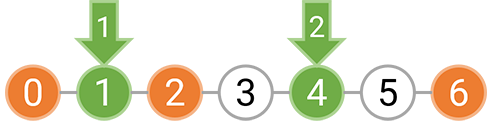
\includegraphics[width=0.95\textwidth]{image/22/4-p-1.png}
    % \caption{神经元 $v$ 变量随时间变化的曲线}
\end{figure}

对区间 $[0, 2)$ 和 $[2, 6)$ 分别以 $1$ 和 $2$ 的间隔种树是美观的

% <img alt="sample2_h.png" src="/RequireFile.do?fid=G97DdvfC"/>
\begin{figure}[H]
    \centering
    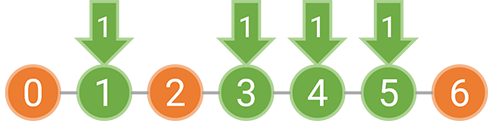
\includegraphics[width=0.95\textwidth]{image/22/4-p-2.png}
    % \caption{神经元 $v$ 变量随时间变化的曲线}
\end{figure}

对区间 $[0, 2)$ 和 $[2, 6)$ 分别以 $1$ 的间隔种树也是美观的

而如果选择在 $[0, 6)$ 区间等间隔种树,我们只能以 $3$ 的间隔种树,因为无论是选择间隔 $1$ 或者间隔 $2$,都需要在坐标 $2$ 上种树,而这个位置已经有障碍物了。下图分别表示了间隔为 $3, 2, 1$ 时的种树情况,红色箭头表示不能在这里种树。

% <img alt="sample3_h.png" src="/RequireFile.do?fid=dAQwSTuu"/>
\begin{figure}[H]
    \centering
    
\includegraphics[width=0.95\textwidth]{image/22/4-p-3.png}
    % \caption{神经元 $v$ 变量随时间变化的曲线}
\end{figure}

对区间 $[0, 6)$ 以 $3$ 的间隔种树是美观的

% <img alt="sample4_h.png" src="/RequireFile.do?fid=hpTkShxA"/>
\begin{figure}[H]
    \centering
    
\includegraphics[width=0.95\textwidth]{image/22/4-p-4.png}
    % \caption{神经元 $v$ 变量随时间变化的曲线}
\end{figure}

对区间 $[0, 6)$ 以 $2$ 的间隔种树是不美观的

% <img alt="sample5_h.png" src="/RequireFile.do?fid=oNrrpgBz"/>
\begin{figure}[H]
    \centering
    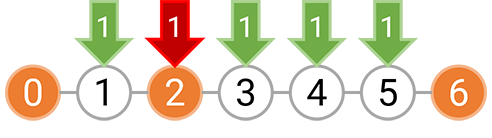
\includegraphics[width=0.95\textwidth]{image/22/4-p-5.png}
    % \caption{神经元 $v$ 变量随时间变化的曲线}
\end{figure}

对区间 $[0, 6)$ 以 $1$ 的间隔种树也是不美观的

一般地,给定一个区间 $[a_l, a_r)$,对于树的坐标的集合 $T\subset(a_l, a_r)$($T\subset\mathbb{Z}$),归纳定义 $T$ 在 $[a_l, a_r)$ 上是{\heiti{美观的}}:

\begin{enumerate}

    \item 如果 $T\ne \emptyset$,$T\cap \left\{a_l, a_{l+1}, \cdots, a_r\right\}=\emptyset$,并且存在一个公差 $d\ge 1$,使得 $T\cup\left\{a_l, a_r\right\}$ 中的元素按照从小到大的顺序排序后,可以构成一个公差为 $d$ 的等差数列(显然,这个等差数列的首项为 $a_l$,末项为 $a_r$),则 $T$ 在 $\left[a_l, a_r\right)$ 上是美观的;

    \item 如果 $T\cap \left\{a_l, a_{l+1}, \cdots, a_r\right\}=\emptyset$,并且存在一个下标 $m$($l<m<r$),使得 $T\cap\left(a_l, a_m\right)$ 在 $\left[a_l, a_m\right)$ 上是美观的,且 $T\cap\left(a_m, a_r\right)$ 在 $\left[a_m, a_r\right)$ 上是美观的,则 $T$ 在 $\left[a_l, a_r\right)$ 上是美观的。

\end{enumerate}

根据这一定义,空集在任意区间上都不是美观的;另外,如果存在下标 $i$ 使得 $a_i \in T$,那么 $T$ 一定不是美观的。

我们称两种种树的方案是{\heiti{本质不同的}},当且仅当两种方案中,种树的坐标集合不同。请帮助 X 校对 $\left[a_1, a_n\right)$ 求出所有本质不同的美观的种树方案。当然,由于方案可能很多,你只需要输出总方案数对 $10^9+7$ 取模的结果。


\subsection*{输入格式}

输入的第一行包含一个正整数 $n$,表示障碍物的数量。

输入的第二行包括 $n$ 个非负整数 $a_1, \cdots, a_n$,表示每个障碍物的坐标。

保证对 $i=1, 2, \cdots, n-1$,$a_i < a_{i+1}$。


\subsection*{输出格式}

输出一个非负整数,表示本质不同的美观的种树方案的数量对 $10^9+7$ 取模的结果。

\examplebox*{\lstinputlisting[frame=none]{data/22/4-1.in}}{\lstinputlisting[frame=none]{data/22/4-1.out}}

这组样例即为题面描述中提到的那组。

\examplebox{\lstinputlisting[frame=none]{data/22/4-2.in}}{\lstinputlisting[frame=none]{data/22/4-2.out}}

\examplebox{见 \href{data/22/4-3.in}{data/22/4-3.in}}{见 \href{data/22/4-3.out}{data/22/4-3.out}}

\subsection*{子任务}

对于 $10\%$ 的数据,保证 $n=2$;

对于 $30\%$ 的数据,保证 $n\le 10$;

对于 $60\%$ 的数据,保证 $n\le 100,a_i\le 1000$;

对于 $1000\%$ 的数据,保证 $2\le n\le 1000,0\le a_i\le 10^5$,且至少存在一种美观的种树方案。

\newpage
\section{202104-5 疫苗运输}
\ifonlyanalyze
\else
  \subsection*{问题描述}

X 市最近生产了一批疫苗,需要运往各地使用。疫苗的运输是一个困难的问题:既要实现尽快时间送达,又要保证全程冷链,否则疫苗会损坏。

X 市的物流系统并不发达,只有 $n$ 个{\heiti{物流站点}}(以下简称“站点”)和 $m$ 条{\heiti{物流线路}}(以下简称“线路”),且该物流系统具有以下几个特点:

\begin{enumerate}

    \item 每条线路都是环线。即,从某个站点出发,经过一系列不重复的站点,最终回到出发站点。

    \item 每条线路上有且仅有一辆{\heiti{运输车}},以固定的时刻表(相邻站间的时间间隔)在环线上不断运行。在 0 时刻时,运输车在出发站点。

    \item 运输车上配备了容量足够大的制冷系统,疫苗可以在车上长时间存放。但是{\heiti{换乘}}(从一条线路切换到另一条线路)必须在同一个站点同一个时刻发生——因为各个站点没有独立的制冷系统,疫苗不能在站点内下车等待。

\end{enumerate}

现在 X 市想要从 1 号站点开始,经过若干条线路的运输和换乘,将疫苗运输到各个其他站点。
与其他站点不同,1 号站点配有冷库。也就是说,从 0 时刻开始,可以在 1 号站点等待某条线路运输车的到来,再开始疫苗运输。
问对于 2 号 ~ $n$ 号站点,分别最早可以在什么{\heiti{时刻}}将疫苗送到该站点。

注意:每个问题是独立的,即只需要求出 1 号站点到各个站点的最早送达时刻。


\subsection*{输入格式}

第一行两个整数 $n$, $m$。

接下来 $m$ 行,每行表示一条物流线路。对于第 $i ~ (1 \le i \le m)$ 条线路,首先有一个整数 $l_i ~ (2 \le l_i \le n)$ 表示该线路经过的站点个数。接下来 $2 l_i$ 个整数,第 $2j-1$ 和第 $2j$ 个整数分别表示该线路的第 $j ~ (1 \le j \le l_i)$ 个站点的编号 $a_{i,j} ~ (1 \le a_{i,j} \le n)$,以及该线路的第 $j$ 个站点到下一个站点所需的时间 $t_{i,j} ~ (1 \le t_{i,j} \le T)$(对于第 $l_i$ 个站点即为它到第 1 个站点的时间)。其中,每条线路的第 1 个站点为其出发站点。输入中同一行相邻的整数,均用一个空格隔开。


\subsection*{输出格式}

输出 $n - 1$ 行,第 $i$ 行表示将疫苗送达第 $i+1$ 个站点的最早时间:
如果能在有限时间内送达,输出最早的送达时刻;否则输出 \verb|inf|。

\examplebox{\lstinputlisting[frame=none]{data/22/5-1.in}}{\lstinputlisting[frame=none]{data/22/5-1.out}}

\examplebox*{\lstinputlisting[frame=none]{data/22/5-2.in}}{\lstinputlisting[frame=none]{data/22/5-2.out}}

在此样例中,有 5 个站点、3 条线路。第一条线路经过站点 1、2、3,第二条线路经过站点 3、4、5,第三条线路经过站点 3 和 5。

以下为从 1 号站点到各个其他站点的最早送达路线:

\begin{itemize}
    \item 2 号站点:通过第一条线路运输,在 100 时刻到达 2 号站点;
    \item 3 号站点:通过第一条线路运输,在 200 时刻到达 3 号站点;
    \item 4 号站点:通过第一条线路运输,在 500 时刻到达 3 号站点,然后换乘第三条线路,在 1500 时刻再次到达 3 号站点,最后换乘第二条线路,在 1600 时刻到达 4 号站点;
    \item 5 号站点:通过第一条线路运输,在 500 时刻到达 3 号站点,然后换乘第三条线路,在 625 时刻到达 5 号站点。
\end{itemize}

\examplebox{\lstinputlisting[frame=none]{data/22/5-3.in}}{\lstinputlisting[frame=none]{data/22/5-3.out}}

\subsection*{子任务}

对于 10\% 的数据,$n\le 5,m=1,T\le 10$。

对于 30\% 的数据,$n\le 5,m\le 2,T\le 10$。

对于 50\% 的数据,$n\le 5,m\le 5,T\le 10$。

对于 70\% 的数据,$n\le 10,m\le 10,T\le 100$。

对于 80\% 的数据,$n\le 30,m\le 30,T\le 1000$。

对于 95\% 的数据,$n\le 100,m\le 100,T\le 10^5$。

对于 100\% 的数据,$n\le 500,m\le 500,T\le 10^6$。
\fi
% \section{202104-5}

% \subsection*{问题描述}

X 市最近生产了一批疫苗,需要运往各地使用。疫苗的运输是一个困难的问题:既要实现尽快时间送达,又要保证全程冷链,否则疫苗会损坏。

X 市的物流系统并不发达,只有 $n$ 个{\heiti{物流站点}}(以下简称“站点”)和 $m$ 条{\heiti{物流线路}}(以下简称“线路”),且该物流系统具有以下几个特点:

\begin{enumerate}

    \item 每条线路都是环线。即,从某个站点出发,经过一系列不重复的站点,最终回到出发站点。

    \item 每条线路上有且仅有一辆{\heiti{运输车}},以固定的时刻表(相邻站间的时间间隔)在环线上不断运行。在 0 时刻时,运输车在出发站点。

    \item 运输车上配备了容量足够大的制冷系统,疫苗可以在车上长时间存放。但是{\heiti{换乘}}(从一条线路切换到另一条线路)必须在同一个站点同一个时刻发生——因为各个站点没有独立的制冷系统,疫苗不能在站点内下车等待。

\end{enumerate}

现在 X 市想要从 1 号站点开始,经过若干条线路的运输和换乘,将疫苗运输到各个其他站点。
与其他站点不同,1 号站点配有冷库。也就是说,从 0 时刻开始,可以在 1 号站点等待某条线路运输车的到来,再开始疫苗运输。
问对于 2 号 ~ $n$ 号站点,分别最早可以在什么{\heiti{时刻}}将疫苗送到该站点。

注意:每个问题是独立的,即只需要求出 1 号站点到各个站点的最早送达时刻。


\subsection*{输入格式}

第一行两个整数 $n$, $m$。

接下来 $m$ 行,每行表示一条物流线路。对于第 $i ~ (1 \le i \le m)$ 条线路,首先有一个整数 $l_i ~ (2 \le l_i \le n)$ 表示该线路经过的站点个数。接下来 $2 l_i$ 个整数,第 $2j-1$ 和第 $2j$ 个整数分别表示该线路的第 $j ~ (1 \le j \le l_i)$ 个站点的编号 $a_{i,j} ~ (1 \le a_{i,j} \le n)$,以及该线路的第 $j$ 个站点到下一个站点所需的时间 $t_{i,j} ~ (1 \le t_{i,j} \le T)$(对于第 $l_i$ 个站点即为它到第 1 个站点的时间)。其中,每条线路的第 1 个站点为其出发站点。输入中同一行相邻的整数,均用一个空格隔开。


\subsection*{输出格式}

输出 $n - 1$ 行,第 $i$ 行表示将疫苗送达第 $i+1$ 个站点的最早时间:
如果能在有限时间内送达,输出最早的送达时刻;否则输出 \verb|inf|。

\examplebox{\lstinputlisting[frame=none]{data/22/5-1.in}}{\lstinputlisting[frame=none]{data/22/5-1.out}}

\examplebox*{\lstinputlisting[frame=none]{data/22/5-2.in}}{\lstinputlisting[frame=none]{data/22/5-2.out}}

在此样例中,有 5 个站点、3 条线路。第一条线路经过站点 1、2、3,第二条线路经过站点 3、4、5,第三条线路经过站点 3 和 5。

以下为从 1 号站点到各个其他站点的最早送达路线:

\begin{itemize}
    \item 2 号站点:通过第一条线路运输,在 100 时刻到达 2 号站点;
    \item 3 号站点:通过第一条线路运输,在 200 时刻到达 3 号站点;
    \item 4 号站点:通过第一条线路运输,在 500 时刻到达 3 号站点,然后换乘第三条线路,在 1500 时刻再次到达 3 号站点,最后换乘第二条线路,在 1600 时刻到达 4 号站点;
    \item 5 号站点:通过第一条线路运输,在 500 时刻到达 3 号站点,然后换乘第三条线路,在 625 时刻到达 5 号站点。
\end{itemize}

\examplebox{\lstinputlisting[frame=none]{data/22/5-3.in}}{\lstinputlisting[frame=none]{data/22/5-3.out}}

\subsection*{子任务}

对于 10\% 的数据,$n\le 5,m=1,T\le 10$。

对于 30\% 的数据,$n\le 5,m\le 2,T\le 10$。

对于 50\% 的数据,$n\le 5,m\le 5,T\le 10$。

对于 70\% 的数据,$n\le 10,m\le 10,T\le 100$。

对于 80\% 的数据,$n\le 30,m\le 30,T\le 1000$。

对于 95\% 的数据,$n\le 100,m\le 100,T\le 10^5$。

对于 100\% 的数据,$n\le 500,m\le 500,T\le 10^6$。

% 第23次认证

\chapter{第23次认证(2021年09月)}

\section{题目及设计知识点}

\begin{table}[htbp]
  \centering
  \begin{tabular}{ccc}
    \toprule
    题目编号 & 题目名称       & 知识点           \\
    \midrule
    1        & 数组推导       & 模拟             \\
    2        & 非零段划分     & 模拟,数学       \\
    3        & 脉冲神经网络   & 模拟             \\
    4        & 收集卡牌       & 状压dp           \\
    5        & 箱根山岳险天下 & 树链剖分,动态树 \\
    \bottomrule
  \end{tabular}
\end{table}

\newpage
\section{202109-1 数组推导}
\ifonlyanalyze
\else
  \subsection*{题目描述}

$A_1, A_2, \cdots, A_n$ 是一个由 $n$ 个{\heiti{自然数}}(即非负整数)组成的数组。
在此基础上,我们用数组 $B_1 \cdots B_n$ 表示 $A$ 的前缀最大值。

\begin{equation*}
    B_i = \max \left\{ A_1, A_2,  \cdots, A_i \right\}
\end{equation*}

如上所示,$B_i$ 定义为数组 $A$ 中前 $i$ 个数的最大值。
根据该定义易知 $A_1 = B_1$,且随着 $i$ 的增大,$B_i$ 单调不降。
此外,我们用 $sum = A_1 + A_2 + \cdots + A_n$ 表示数组 $A$ 中 $n$ 个数的总和。

现已知数组 $B$,我们想要根据 $B$ 的值来反推数组 $A$。
显然,对于给定的 $B$,$A$ 的取值可能并不唯一。
试计算,在数组 $A$ 所有可能的取值情况中,$sum$ 的最大值和最小值分别是多少?

\subsection*{输入格式}

从标准输入读入数据。

输入的第一行包含一个正整数 $n$。

输入的第二行包含 $n$ 个用空格分隔的自然数 $B_1, B_2, \cdots, B_n$。

\subsection*{输出格式}

输出到标准输出。

输出共两行。

第一行输出一个整数,表示 $sum$ 的最大值。

第二行输出一个整数,表示 $sum$ 的最小值。

\examplebox*{\lstinputlisting[frame=none]{data/23/1-1.in}}{\lstinputlisting[frame=none]{data/23/1-1.out}}

数组 $A$ 的可能取值包括但不限于以下三种情况。

\begin{itemize}
    \item 情况一:$A = [0, 0, 5, 5, 10, 10]$
    \item 情况二:$A = [0, 0, 5, 3, 10, 4]$
    \item 情况三:$A = [0, 0, 5, 0, 10, 0]$
\end{itemize}

其中第一种情况 $sum = 30$ 为最大值,第三种情况 $sum = 15$ 为最小值。

\examplebox*{\lstinputlisting[frame=none]{data/23/1-2.in}}{\lstinputlisting[frame=none]{data/23/1-2.out}}

$A = [10, 20, 30, 40, 50, 60, 75]$ 是唯一可能的取值,所以 $sum$ 的最大、最小值均为 $285$。

\subsection*{子任务}

$50\%$ 的测试数据满足数组 $B$ 单调递增,即 $0 < B_1 < B_2 < \cdots < B_n < 10^{5}$;

全部的测试数据满足 $n \le 100$ 且数组 $B$ 单调不降,即 $0 \le B_1 \le B_2 \le \cdots \le B_n \le 10^{5}$。



\fi
% \section{202109-1 数组推导}

% \subsection*{题目描述}

$A_1, A_2, \cdots, A_n$ 是一个由 $n$ 个{\heiti{自然数}}(即非负整数)组成的数组。
在此基础上,我们用数组 $B_1 \cdots B_n$ 表示 $A$ 的前缀最大值。

\begin{equation*}
    B_i = \max \left\{ A_1, A_2,  \cdots, A_i \right\}
\end{equation*}

如上所示,$B_i$ 定义为数组 $A$ 中前 $i$ 个数的最大值。
根据该定义易知 $A_1 = B_1$,且随着 $i$ 的增大,$B_i$ 单调不降。
此外,我们用 $sum = A_1 + A_2 + \cdots + A_n$ 表示数组 $A$ 中 $n$ 个数的总和。

现已知数组 $B$,我们想要根据 $B$ 的值来反推数组 $A$。
显然,对于给定的 $B$,$A$ 的取值可能并不唯一。
试计算,在数组 $A$ 所有可能的取值情况中,$sum$ 的最大值和最小值分别是多少?

\subsection*{输入格式}

从标准输入读入数据。

输入的第一行包含一个正整数 $n$。

输入的第二行包含 $n$ 个用空格分隔的自然数 $B_1, B_2, \cdots, B_n$。

\subsection*{输出格式}

输出到标准输出。

输出共两行。

第一行输出一个整数,表示 $sum$ 的最大值。

第二行输出一个整数,表示 $sum$ 的最小值。

\examplebox*{\lstinputlisting[frame=none]{data/23/1-1.in}}{\lstinputlisting[frame=none]{data/23/1-1.out}}

数组 $A$ 的可能取值包括但不限于以下三种情况。

\begin{itemize}
    \item 情况一:$A = [0, 0, 5, 5, 10, 10]$
    \item 情况二:$A = [0, 0, 5, 3, 10, 4]$
    \item 情况三:$A = [0, 0, 5, 0, 10, 0]$
\end{itemize}

其中第一种情况 $sum = 30$ 为最大值,第三种情况 $sum = 15$ 为最小值。

\examplebox*{\lstinputlisting[frame=none]{data/23/1-2.in}}{\lstinputlisting[frame=none]{data/23/1-2.out}}

$A = [10, 20, 30, 40, 50, 60, 75]$ 是唯一可能的取值,所以 $sum$ 的最大、最小值均为 $285$。

\subsection*{子任务}

$50\%$ 的测试数据满足数组 $B$ 单调递增,即 $0 < B_1 < B_2 < \cdots < B_n < 10^{5}$;

全部的测试数据满足 $n \le 100$ 且数组 $B$ 单调不降,即 $0 \le B_1 \le B_2 \le \cdots \le B_n \le 10^{5}$。




\subsection{\texorpdfstring{$100\%$}{100\%} 数据——模拟}

\subsubsection{思路}

$B$ 数组是 $A$ 数组的前缀最大值,所以 $B$ 必定是单调不降的。

考虑 $B$ 数组中相邻元素之间的关系,推测 $A$ 数组中的元素值范围:

\begin{itemize}
    \item $B_1=A_1$;
    \item 若 $B_i\not=B_{i-1}(i\ge 2)$,说明前缀最大值在第 $i$ 个位置发生了改变;
          考虑 $A_i$:若 $A_i \le B_{i-1}$ 则 $B_i$ 不会发生变化,
          若 $A_i > B_{i-1}$ 且 $A_i\not=B_i$ 则 $B_i=A_i$ 矛盾,
          所以此时 $B_i=A_i$;
    \item 若 $B_i=B_{i-1}(i\ge 2)$,说明前缀最大值在 $i$ 处没有改变,结合上面的分析
          我们可以得到 $A_i \in [0, B_{i-1}]$。
\end{itemize}

综合以上分析,只有在 $B_{i}=B_{i-1}(i\ge 2)$ 时,$A_i$ 的值是不确定的。
要求最大最小值,只要令不确定的 $A_i=0$ 或 $A_i=B_{i-1}$ 即可。

\newpage
\section{202109-2 非零段划分}
\ifonlyanalyze
\else
  \subsection*{题目描述}

$A_1, A_2, \cdots, A_n$ 是一个由 $n$ 个自然数(非负整数)组成的数组。
我们称其中 $A_i, \cdots, A_j$ 是一个非零段,当且仅当以下条件同时满足:

\begin{itemize}
    \item $1 \le i \le j \le n$;
    \item 对于任意的整数 $k$,若 $i \le k \le j$,则 $A_k > 0$;
    \item $i = 1$ 或 $A_{i-1} = 0$;
    \item $j = n$ 或 $A_{j+1} = 0$。
\end{itemize}

下面展示了几个简单的例子:

\begin{itemize}
    \item $A = [3, 1, 2, 0, 0, 2, 0, 4, 5, 0, 2]$ 中的 $4$ 个非零段依次为 $[3, 1, 2]$、$[2]$、$[4, 5]$ 和 $[2]$;
    \item $A = [2, 3, 1, 4, 5]$ 仅有 $1$ 个非零段;
    \item $A = [0, 0, 0]$ 则不含非零段(即非零段个数为 $0$)。
\end{itemize}

现在我们可以对数组 $A$ 进行如下操作:
任选一个正整数 $p$,然后将 $A$ 中所有小于 $p$ 的数都变为 $0$。
试选取一个合适的 $p$,使得数组 $A$ 中的非零段个数达到最大。
若输入的 $A$ 所含非零段数已达最大值,可取 $p=1$,即不对 $A$ 做任何修改。

\subsection*{输入格式}

从标准输入读入数据。

输入的第一行包含一个正整数 $n$。

输入的第二行包含 $n$ 个用空格分隔的自然数 $A_1, A_2, \cdots, A_n$。

\subsection*{输出格式}

输出到标准输出。

仅输出一个整数,表示对数组 $A$ 进行操作后,其非零段个数能达到的最大值。

\examplebox*{\lstinputlisting[frame=none]{data/23/2-1.in}}{\lstinputlisting[frame=none]{data/23/2-1.out}}

$p = 2$ 时,$A = [3, 0, 2, 0, 0, 2, 0, 4, 5, 0, 2]$,$5$ 个非零段依次为 $[3]$、$[2]$、$[2]$、$[4, 5]$ 和 $[2]$;此时非零段个数达到最大。

\examplebox*{\lstinputlisting[frame=none]{data/23/2-2.in}}{\lstinputlisting[frame=none]{data/23/2-2.out}}

$p = 12$ 时,$A = [0, 0, 20, 0, 0, 0, 0, 15, 0, 20, 0, 0, 0, 15]$,$4$ 个非零段依次为 $[20]$、$[15]$、$[20]$ 和 $[15]$;此时非零段个数达到最大。

\examplebox*{\lstinputlisting[frame=none]{data/23/2-3.in}}{\lstinputlisting[frame=none]{data/23/2-3.out}}

$p = 1$ 时,$A = [1, 0, 0]$,此时仅有 $1$ 个非零段 $[1]$,非零段个数达到最大。

\examplebox*{\lstinputlisting[frame=none]{data/23/2-4.in}}{\lstinputlisting[frame=none]{data/23/2-4.out}}

无论 $p$ 取何值,$A$ 都不含有非零段,故非零段个数至多为 $0$。

\subsection*{子任务}

$70\%$ 的测试数据满足 $n \le 1000$;

全部的测试数据满足 $n \le 5 \times 10^{5}$,且数组 $A$ 中的每一个数均不超过 $10^{4}$。



\fi
% \section{202109-2 非零段划分}

% \subsection*{题目描述}

$A_1, A_2, \cdots, A_n$ 是一个由 $n$ 个自然数(非负整数)组成的数组。
我们称其中 $A_i, \cdots, A_j$ 是一个非零段,当且仅当以下条件同时满足:

\begin{itemize}
    \item $1 \le i \le j \le n$;
    \item 对于任意的整数 $k$,若 $i \le k \le j$,则 $A_k > 0$;
    \item $i = 1$ 或 $A_{i-1} = 0$;
    \item $j = n$ 或 $A_{j+1} = 0$。
\end{itemize}

下面展示了几个简单的例子:

\begin{itemize}
    \item $A = [3, 1, 2, 0, 0, 2, 0, 4, 5, 0, 2]$ 中的 $4$ 个非零段依次为 $[3, 1, 2]$、$[2]$、$[4, 5]$ 和 $[2]$;
    \item $A = [2, 3, 1, 4, 5]$ 仅有 $1$ 个非零段;
    \item $A = [0, 0, 0]$ 则不含非零段(即非零段个数为 $0$)。
\end{itemize}

现在我们可以对数组 $A$ 进行如下操作:
任选一个正整数 $p$,然后将 $A$ 中所有小于 $p$ 的数都变为 $0$。
试选取一个合适的 $p$,使得数组 $A$ 中的非零段个数达到最大。
若输入的 $A$ 所含非零段数已达最大值,可取 $p=1$,即不对 $A$ 做任何修改。

\subsection*{输入格式}

从标准输入读入数据。

输入的第一行包含一个正整数 $n$。

输入的第二行包含 $n$ 个用空格分隔的自然数 $A_1, A_2, \cdots, A_n$。

\subsection*{输出格式}

输出到标准输出。

仅输出一个整数,表示对数组 $A$ 进行操作后,其非零段个数能达到的最大值。

\examplebox*{\lstinputlisting[frame=none]{data/23/2-1.in}}{\lstinputlisting[frame=none]{data/23/2-1.out}}

$p = 2$ 时,$A = [3, 0, 2, 0, 0, 2, 0, 4, 5, 0, 2]$,$5$ 个非零段依次为 $[3]$、$[2]$、$[2]$、$[4, 5]$ 和 $[2]$;此时非零段个数达到最大。

\examplebox*{\lstinputlisting[frame=none]{data/23/2-2.in}}{\lstinputlisting[frame=none]{data/23/2-2.out}}

$p = 12$ 时,$A = [0, 0, 20, 0, 0, 0, 0, 15, 0, 20, 0, 0, 0, 15]$,$4$ 个非零段依次为 $[20]$、$[15]$、$[20]$ 和 $[15]$;此时非零段个数达到最大。

\examplebox*{\lstinputlisting[frame=none]{data/23/2-3.in}}{\lstinputlisting[frame=none]{data/23/2-3.out}}

$p = 1$ 时,$A = [1, 0, 0]$,此时仅有 $1$ 个非零段 $[1]$,非零段个数达到最大。

\examplebox*{\lstinputlisting[frame=none]{data/23/2-4.in}}{\lstinputlisting[frame=none]{data/23/2-4.out}}

无论 $p$ 取何值,$A$ 都不含有非零段,故非零段个数至多为 $0$。

\subsection*{子任务}

$70\%$ 的测试数据满足 $n \le 1000$;

全部的测试数据满足 $n \le 5 \times 10^{5}$,且数组 $A$ 中的每一个数均不超过 $10^{4}$。




\subsection{\texorpdfstring{$70\%$}{70\%} 数据——模拟}

\subsubsection{思路}

题目中说明 $A_i\in[0, 10000]$。当 $p>10000$ 后,$A$ 数组则成为全 $0$ 数组,
所以我们只需考虑 $k\in[1, 10000]$ 时的非零段个数,不妨设 $m=10000$。

我们可以针对每一个 $p$,计算出 $A$ 数组的情况,进而计算非零段的个数,不断更新答案。
在维护 $A$ 数组的时候,我们可以让 $p$ 递增更新。
这样在 $p$ 更新的时候,只需要将 $A_i=p-1$ 处更新为 $0$ 即可。

时间复杂度 $\mathrm{O}(nm)$。

\subsection{\texorpdfstring{$100\%$}{100\%} 数据——避免不必要更新}

\subsubsection{思路}

在上个做法中,时间主要浪费在了对 $A$ 数组的更新与重复计算非零段上。
对于每一个非零 $A_i$,随着 $p$ 逐渐增大,其最多改变一次,即变为 $0$。
而在上面的方法中,我们忽略了这个条件,每次都对所有的元素进行检查,无论其是否为 $0$。

考虑每个 $A_i$ 变为 $0$ 时对非零段个数的贡献。
为了简化后续讨论,这里给出一个推论:

\begin{corollary}[相邻相等元素与单个元素等价] \label{cor:adjacent-same-element-equals-one-element}
    对于一段值相同的区间,可以把它们看做成其中任意的一个元素。

    这一点很好理解:既然值相同,那么这一段在变为 $0$ 时必然是同时改变。
\end{corollary}

通过以上推论,我们先缩小 $A$ 数组的元素个数,直到任意相邻两个元素都不同,之后考虑每个元素对整体的贡献。
只看元素本身看不出什么,一种思路是查看与之相邻的两个元素。

\begin{figure}[H]
    \centering
    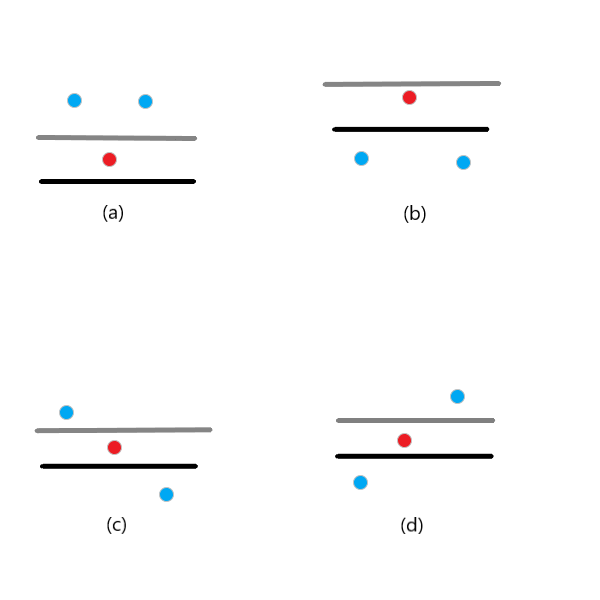
\includegraphics[width=0.6\textwidth]{image/23/2-1.png}
    \caption{相邻元素的四种情况}
\end{figure}

如图,红色点代表将要变为 $0$ 的元素,蓝色点为相邻两个元素;黑线以下为目前变为 $0$ 的元素。我们对以上四种情况进行分类讨论:

\begin{enumerate}
    \item 当左右相邻元素均大于中间元素时:当中间元素变为 $0$ 时,原本一个非零段分成了两个非零段,对非零段个数贡献 $+1$;
    \item 当左右相邻元素均小于中间元素时:当中间元素变为 $0$ 之前,左右元素均已变成 $0$,中间元素是孤立的非零段,在中间元素变为 $0$ 后,非零段个数减少,对非零段个数贡献 $-1$;
    \item 其他两种情况:相当于某个非零段的边界去掉了一个元素,对非零段个数无影响。
\end{enumerate}

针对边界元素而言,可以将其缺失的相邻元素视为 $0$。

同时,考虑到我们只需要求解非零段的个数,并不需要输出对应 $A$ 数组的状态,我们可以将每个元素的贡献(当然只有在对应 $p=A_{i}+1$ 时才会有贡献)累加,成为每个 $p$ 对应的贡献。
这样我们就可以先求出初始状态的非零段个数,之后随着 $p$ 增加利用之前求出的贡献进行更新,就可以比较快速地解决。

求出每个元素的贡献、并累加到对应 $p$ 的复杂度为 $\mathrm{O}(n)$,计算每一个 $p$ 的最后贡献的复杂度为 $\mathrm{O}(m)$,整体复杂度 $\mathrm{O}(n+m)$。

\subsubsection{C++实现}

\lstinputlisting[language=c++]{code/23/202109-2-100.cpp}

\newpage
\section{202109-3 脉冲神经网络}
\ifonlyanalyze
\else
  \subsection*{题目背景}

在本题中,你需要实现一个 SNN(spiking neural network,脉冲神经网络)的模拟器。一个 SNN 由以下几部分组成:

\begin{enumerate}
    \item 神经元:按照一定的公式更新内部状态,接受脉冲并可以发放脉冲
    \item 脉冲源:在特定的时间发放脉冲
    \item 突触:连接神经元-神经元或者脉冲源-神经元,负责传递脉冲
\end{enumerate}

\subsection*{题目描述}


神经元会按照一定的规则更新自己的内部状态。本题中,我们对时间进行离散化处理,即设置一个时间间隔 $\Delta{t}$,仅考虑时间间隔整数倍的时刻 $t=k\Delta{t}(k \in Z^+)$,按照下面的公式,从 $k-1$ 时刻的取值计算 $k$ 时刻的变量的取值:

\begin{equation*}
    v_k=v_{k-1} + \Delta{t}(0.04v_{k-1}^2 + 5v_{k-1} + 140 - u_{k-1}) + I_k
\end{equation*}

\begin{equation*}
    u_k=u_{k-1} + \Delta{t}a(bv_{k-1} - u_{k-1})
\end{equation*}

其中 $v$ 和 $u$ 是神经元内部的变量,会随着时间而变化,$a$ 和 $b$ 是常量,不会随着时间变化;其中 $I_k$ 表示该神经元在 $k$ 时刻接受到的所有脉冲输入的强度之和,如果没有接受到脉冲,那么 $I_k=0$。当进行上面的计算后,如果满足 $v_k \ge 30$,神经元会发放一个脉冲,脉冲经过突触传播到其他神经元;同时,$v_k$ 设为 $c$ 并且 $u_k$ 设为 $u_k + d$,其中 $c$ 和 $d$ 也是常量。图 1 展示了一个神经元 $v$ 变量随时间变化的曲线。

\begin{figure}[H]
    \centering
    \includegraphics[width=0.95\textwidth]{image/23/3-p-1.png}
    \caption{神经元 $v$ 变量随时间变化的曲线}
\end{figure}

突触表示的是神经元-神经元、脉冲源-神经元的连接关系,包含一个入结点和一个出结点(可能出现自环和重边)。当突触的入结点(神经元或者脉冲源)在 $k$ 时刻发放一个脉冲,那么在传播延迟 $D(D > 0)$ 个时刻以后,也就是在 $k+D$ 时刻突触的出结点(神经元)会接受到一个强度为 $w$ 的脉冲。

脉冲源在每个时刻以一定的概率发放一个脉冲,为了模拟这个过程,每个脉冲源有一个参数 $0 < r \le 32,767$,并统一采用以下的伪随机函数:

C++ 版本:

\begin{lstlisting}[language=c++]
static unsigned long next = 1;

/* RAND_MAX assumed to be 32767 */
int myrand(void) {
    next = next * 1103515245 + 12345;
    return((unsigned)(next/65536) % 32768);
}
\end{lstlisting}

Python 版本:

\begin{lstlisting}[language=python]
next = 1
def myrand():
    global next
    next = (next * 1103515245 + 12345) % (2 ** 64)
    return (next // 65536) % 32768
\end{lstlisting}

Java 版本:

\begin{lstlisting}[language=java]
long next = 1;
int myrand() {
    next = next * 1103515245 + 12345;
    return (int)((Long.divideUnsigned(next, 65536)) % 32768);
}
\end{lstlisting}

在每个时间刻,按照编号顺序从小到大,每个脉冲源调用一次上述的伪随机函数,当 $r > \text{myrand()}$ 时,在当前时间刻发放一次脉冲,并通过突触传播到神经元。

进行仿真的时候,已知 0 时间刻各个神经元的状态,从 1 时间刻开始按照上述规则进行计算,直到完成 $T$ 时刻的计算,再输出 $T$ 时刻神经元的 $v$ 值和发放的脉冲次数分别的最小值和最大值。

规定输入数据中结点按如下方式顺序编号:$[0, N-1]$ 为神经元的编号,$[N, N+P-1]$ 为脉冲源的编号。

代码中请使用双精度浮点类型。

\subsection*{输入格式}

从标准输入读入数据。

输入的第一行包括四个以空格分隔的正整数 $N$ $S$ $P$ $T$,表示一共有 $N$ 个神经元,$S$ 个突触和 $P$ 个脉冲源,输出时间刻 $T$ 时神经元的 $v$ 值。

输入的第二行是一个正实数 $\Delta{t}$,表示时间间隔。

输入接下来的若干行,每行有以空格分隔的一个正整数 $R_N$ 和六个实数 $v$ $u$ $a$ $b$ $c$ $d$,按顺序每一行对应 $R_N$ 个具有相同初始状态和常量的神经元:其中 $v$ $u$ 表示神经元在时刻 0 时的变量取值;$a$ $b$ $c$ $d$ 为该神经元微分方程里的四个常量。保证所有的 $R_N$ 加起来等于 $N$。它们从前向后按编号顺序描述神经元,每行对应一段连续编号的神经元的信息。

输入接下来的 $P$ 行,每行是一个正整数 $r$,按顺序每一行对应一个脉冲源的 $r$ 参数。

输入接下来的 $S$ 行,每行有以空格分隔的两个整数 $s(0 \le s < N+P)$、$t(0 \le t < N)$ 、一个实数 $w(w \ge 0)$ 和一个正整数 $D$,其中 $s$ 和 $t$ 分别是入结点和出结点的编号;$w$ 和 $D$ 分别表示脉冲强度和传播延迟。

\subsection*{输出格式}

输出到标准输出。

输出共有两行,第一行由两个近似保留 3 位小数的实数组成,分别是所有神经元在时刻 $T$ 时变量 $v$ 的取值的最小值和最大值。第二行由两个整数组成,分别是所有神经元在整个模拟过程中发放脉冲次数的最小值和最大值。

只要按照题目要求正确实现就能通过,不会因为计算精度的问题而得到错误答案。

\examplebox*{\lstinputlisting[frame=none]{data/23/3-1.in}}{\lstinputlisting[frame=none]{data/23/3-1.out}}

该样例有 1 个神经元、1 个突触和 1 个脉冲源,时间间隔 $\Delta{t}=0.1$。唯一的脉冲源通过脉冲强度为 30.0、传播延迟为 2 的突触传播到唯一的神经元。

该样例一共进行 10 个时间步的模拟,随机数生成器生成 10 次随机数如下:

\begin{lstlisting}
16838
5758
10113
17515
31051
5627
23010
7419
16212
4086
\end{lstlisting}

因此唯一的脉冲源在时刻 1-4 和 6-10 发放脉冲。在时间刻从 1 到 10 时,唯一的神经元的 $v$ 取值分别为:

\begin{lstlisting}
-70.000
-70.000
-40.000
-8.200
-65.000
-35.404
-32.895
0.181
-65.000
-35.608
\end{lstlisting}

该神经元在时刻 5 和时刻 9 发放,最终得到的 $v=-35.608$ 。

\examplebox{\lstinputlisting[frame=none]{data/23/3-1.in}}{\lstinputlisting[frame=none]{data/23/3-1.out}}

\subsection*{子任务}

\begin{table}[H]
\centering
\begin{tabular}{ccccccc}
    \toprule
    子任务 & $T$ & $N$ & $S$ & $P$ & $D$ & 分值 \\
    \midrule
    $1$ & $\le 10^2$ & $\le 10^2$ & $\le 10^2$ & $\le 10^2$ & $\le 10^2$ & $30$ \\
    $2$ & $\le 10^3$ & $\le 10^3$ & $\le 10^3$ & $\le 10^3$ & $\le 10^3$ & $40$ \\
    $3$ & $\le 10^5$ & $\le 10^3$ & $\le 10^3$ & $\le 10^3$ & $\le 10$ & $30$ \\
    \bottomrule
\end{tabular}
\end{table}


\fi
% \section{202109-3 脉冲神经网络}

% \subsection*{题目背景}

在本题中,你需要实现一个 SNN(spiking neural network,脉冲神经网络)的模拟器。一个 SNN 由以下几部分组成:

\begin{enumerate}
    \item 神经元:按照一定的公式更新内部状态,接受脉冲并可以发放脉冲
    \item 脉冲源:在特定的时间发放脉冲
    \item 突触:连接神经元-神经元或者脉冲源-神经元,负责传递脉冲
\end{enumerate}

\subsection*{题目描述}


神经元会按照一定的规则更新自己的内部状态。本题中,我们对时间进行离散化处理,即设置一个时间间隔 $\Delta{t}$,仅考虑时间间隔整数倍的时刻 $t=k\Delta{t}(k \in Z^+)$,按照下面的公式,从 $k-1$ 时刻的取值计算 $k$ 时刻的变量的取值:

\begin{equation*}
    v_k=v_{k-1} + \Delta{t}(0.04v_{k-1}^2 + 5v_{k-1} + 140 - u_{k-1}) + I_k
\end{equation*}

\begin{equation*}
    u_k=u_{k-1} + \Delta{t}a(bv_{k-1} - u_{k-1})
\end{equation*}

其中 $v$ 和 $u$ 是神经元内部的变量,会随着时间而变化,$a$ 和 $b$ 是常量,不会随着时间变化;其中 $I_k$ 表示该神经元在 $k$ 时刻接受到的所有脉冲输入的强度之和,如果没有接受到脉冲,那么 $I_k=0$。当进行上面的计算后,如果满足 $v_k \ge 30$,神经元会发放一个脉冲,脉冲经过突触传播到其他神经元;同时,$v_k$ 设为 $c$ 并且 $u_k$ 设为 $u_k + d$,其中 $c$ 和 $d$ 也是常量。图 1 展示了一个神经元 $v$ 变量随时间变化的曲线。

\begin{figure}[H]
    \centering
    \includegraphics[width=0.95\textwidth]{image/23/3-p-1.png}
    \caption{神经元 $v$ 变量随时间变化的曲线}
\end{figure}

突触表示的是神经元-神经元、脉冲源-神经元的连接关系,包含一个入结点和一个出结点(可能出现自环和重边)。当突触的入结点(神经元或者脉冲源)在 $k$ 时刻发放一个脉冲,那么在传播延迟 $D(D > 0)$ 个时刻以后,也就是在 $k+D$ 时刻突触的出结点(神经元)会接受到一个强度为 $w$ 的脉冲。

脉冲源在每个时刻以一定的概率发放一个脉冲,为了模拟这个过程,每个脉冲源有一个参数 $0 < r \le 32,767$,并统一采用以下的伪随机函数:

C++ 版本:

\begin{lstlisting}[language=c++]
static unsigned long next = 1;

/* RAND_MAX assumed to be 32767 */
int myrand(void) {
    next = next * 1103515245 + 12345;
    return((unsigned)(next/65536) % 32768);
}
\end{lstlisting}

Python 版本:

\begin{lstlisting}[language=python]
next = 1
def myrand():
    global next
    next = (next * 1103515245 + 12345) % (2 ** 64)
    return (next // 65536) % 32768
\end{lstlisting}

Java 版本:

\begin{lstlisting}[language=java]
long next = 1;
int myrand() {
    next = next * 1103515245 + 12345;
    return (int)((Long.divideUnsigned(next, 65536)) % 32768);
}
\end{lstlisting}

在每个时间刻,按照编号顺序从小到大,每个脉冲源调用一次上述的伪随机函数,当 $r > \text{myrand()}$ 时,在当前时间刻发放一次脉冲,并通过突触传播到神经元。

进行仿真的时候,已知 0 时间刻各个神经元的状态,从 1 时间刻开始按照上述规则进行计算,直到完成 $T$ 时刻的计算,再输出 $T$ 时刻神经元的 $v$ 值和发放的脉冲次数分别的最小值和最大值。

规定输入数据中结点按如下方式顺序编号:$[0, N-1]$ 为神经元的编号,$[N, N+P-1]$ 为脉冲源的编号。

代码中请使用双精度浮点类型。

\subsection*{输入格式}

从标准输入读入数据。

输入的第一行包括四个以空格分隔的正整数 $N$ $S$ $P$ $T$,表示一共有 $N$ 个神经元,$S$ 个突触和 $P$ 个脉冲源,输出时间刻 $T$ 时神经元的 $v$ 值。

输入的第二行是一个正实数 $\Delta{t}$,表示时间间隔。

输入接下来的若干行,每行有以空格分隔的一个正整数 $R_N$ 和六个实数 $v$ $u$ $a$ $b$ $c$ $d$,按顺序每一行对应 $R_N$ 个具有相同初始状态和常量的神经元:其中 $v$ $u$ 表示神经元在时刻 0 时的变量取值;$a$ $b$ $c$ $d$ 为该神经元微分方程里的四个常量。保证所有的 $R_N$ 加起来等于 $N$。它们从前向后按编号顺序描述神经元,每行对应一段连续编号的神经元的信息。

输入接下来的 $P$ 行,每行是一个正整数 $r$,按顺序每一行对应一个脉冲源的 $r$ 参数。

输入接下来的 $S$ 行,每行有以空格分隔的两个整数 $s(0 \le s < N+P)$、$t(0 \le t < N)$ 、一个实数 $w(w \ge 0)$ 和一个正整数 $D$,其中 $s$ 和 $t$ 分别是入结点和出结点的编号;$w$ 和 $D$ 分别表示脉冲强度和传播延迟。

\subsection*{输出格式}

输出到标准输出。

输出共有两行,第一行由两个近似保留 3 位小数的实数组成,分别是所有神经元在时刻 $T$ 时变量 $v$ 的取值的最小值和最大值。第二行由两个整数组成,分别是所有神经元在整个模拟过程中发放脉冲次数的最小值和最大值。

只要按照题目要求正确实现就能通过,不会因为计算精度的问题而得到错误答案。

\examplebox*{\lstinputlisting[frame=none]{data/23/3-1.in}}{\lstinputlisting[frame=none]{data/23/3-1.out}}

该样例有 1 个神经元、1 个突触和 1 个脉冲源,时间间隔 $\Delta{t}=0.1$。唯一的脉冲源通过脉冲强度为 30.0、传播延迟为 2 的突触传播到唯一的神经元。

该样例一共进行 10 个时间步的模拟,随机数生成器生成 10 次随机数如下:

\begin{lstlisting}
16838
5758
10113
17515
31051
5627
23010
7419
16212
4086
\end{lstlisting}

因此唯一的脉冲源在时刻 1-4 和 6-10 发放脉冲。在时间刻从 1 到 10 时,唯一的神经元的 $v$ 取值分别为:

\begin{lstlisting}
-70.000
-70.000
-40.000
-8.200
-65.000
-35.404
-32.895
0.181
-65.000
-35.608
\end{lstlisting}

该神经元在时刻 5 和时刻 9 发放,最终得到的 $v=-35.608$ 。

\examplebox{\lstinputlisting[frame=none]{data/23/3-1.in}}{\lstinputlisting[frame=none]{data/23/3-1.out}}

\subsection*{子任务}

\begin{table}[H]
\centering
\begin{tabular}{ccccccc}
    \toprule
    子任务 & $T$ & $N$ & $S$ & $P$ & $D$ & 分值 \\
    \midrule
    $1$ & $\le 10^2$ & $\le 10^2$ & $\le 10^2$ & $\le 10^2$ & $\le 10^2$ & $30$ \\
    $2$ & $\le 10^3$ & $\le 10^3$ & $\le 10^3$ & $\le 10^3$ & $\le 10^3$ & $40$ \\
    $3$ & $\le 10^5$ & $\le 10^3$ & $\le 10^3$ & $\le 10^3$ & $\le 10$ & $30$ \\
    \bottomrule
\end{tabular}
\end{table}



\newpage
\section{202109-4 收集卡牌}
\ifonlyanalyze
\else
  \subsection*{题目描述}

小林在玩一个抽卡游戏,其中有 $n$ 种不同的卡牌,编号为 $1$ 到 $n$。每一次抽卡,她获得第 $i$ 种卡牌的概率为 $p_i$。如果这张卡牌之前已经获得过了,就会转化为一枚硬币。可以用 $k$ 枚硬币交换一张没有获得过的卡。

小林会一直抽卡,直至集齐了所有种类的卡牌为止,求她的期望抽卡次数。如果你给出的答案与标准答案的绝对误差不超过 $10^{-4}$,则视为正确。

提示:聪明的小林会把硬币攒在手里,等到通过兑换就可以获得剩余所有卡牌时,一次性兑换并停止抽卡。

\subsection*{输入格式}

从标准输入读入数据。

输入共两行。第一行包含两个用空格分隔的正整数 $n, k$,第二行给出 $p_1, p_2, \dots, p_n$,用空格分隔。

\subsection*{输出格式}

输出到标准输出。

输出共一行,一个实数,即期望抽卡次数。

\subsection*{样例}

输入\#1:

\begin{lstlisting}
2 2
0.4 0.6
\end{lstlisting}

输出\#1:

\begin{lstlisting}
2.52
\end{lstlisting}

解释\#1:

共有 $2$ 种卡牌,不妨记为 A 和 B,获得概率分别为 $0.4$ 和 $0.6$,$2$ 枚硬币可以换一张卡牌。下面给出各种可能出现的情况:

\begin{enumerate}
    \item 第一次抽卡获得 A,第二次抽卡获得 B,抽卡结束,概率为 $0.4 \times 0.6 = 0.24$,抽卡次数为 $2$。
    \item 第一次抽卡获得 A,第二次抽卡获得 A,第三次抽卡获得 B,抽卡结束,概率为 $0.4 \times 0.4 \times 0.6 = 0.096$,抽卡次数为 $3$。
    \item 第一次抽卡获得 A,第二次抽卡获得 A,第三次抽卡获得 A,用硬币兑换 B,抽卡结束,概率为 $0.4 \times 0.4 \times 0.4 = 0.064$,抽卡次数为 $3$。
    \item 第一次抽卡获得 B,第二次抽卡获得 A,抽卡结束,概率为 $0.6 \times 0.4 = 0.24$,抽卡次数为 $2$。
    \item 第一次抽卡获得 B,第二次抽卡获得 B,第三次抽卡获得 A,抽卡结束,概率为 $0.6 \times 0.6 \times 0.4 = 0.144$,抽卡次数为 $3$。
    \item 第一次抽卡获得 B,第二次抽卡获得 B,第三次抽卡获得 B,用硬币兑换 A,抽卡结束,概率为 $0.6 \times 0.6 \times 0.6 = 0.216$,抽卡次数为 $3$。
\end{enumerate}

因此答案是 $0.24 \times 2 + 0.096 \times 3 + 0.064 \times 3 + 0.24 \times 2 + 0.144 \times 3 + 0.216 \times 3 = 2.52$。

输入\#2:

\begin{lstlisting}
4 3
0.006 0.1 0.2 0.694
\end{lstlisting}

输出\#2:

\begin{lstlisting}
7.3229920752
\end{lstlisting}

\subsection*{子任务}

对于 $20\%$ 的数据,保证 $1 \leq n, k \leq 5$。

对于另外 $20\%$ 的数据,保证所有 $p_i$ 是相等的。

对于 $100\%$ 的数据,保证 $1 \leq n \leq 16, 1 \leq k \leq 5$,所有的 $p_i$ 满足 $p_i \geq \frac{1}{10000}$,且 $\sum_{i=1}^{n} p_i=1$。


\fi
% \section{202109-4 收集卡牌}

% \subsection*{题目描述}

小林在玩一个抽卡游戏,其中有 $n$ 种不同的卡牌,编号为 $1$ 到 $n$。每一次抽卡,她获得第 $i$ 种卡牌的概率为 $p_i$。如果这张卡牌之前已经获得过了,就会转化为一枚硬币。可以用 $k$ 枚硬币交换一张没有获得过的卡。

小林会一直抽卡,直至集齐了所有种类的卡牌为止,求她的期望抽卡次数。如果你给出的答案与标准答案的绝对误差不超过 $10^{-4}$,则视为正确。

提示:聪明的小林会把硬币攒在手里,等到通过兑换就可以获得剩余所有卡牌时,一次性兑换并停止抽卡。

\subsection*{输入格式}

从标准输入读入数据。

输入共两行。第一行包含两个用空格分隔的正整数 $n, k$,第二行给出 $p_1, p_2, \dots, p_n$,用空格分隔。

\subsection*{输出格式}

输出到标准输出。

输出共一行,一个实数,即期望抽卡次数。

\subsection*{样例}

输入\#1:

\begin{lstlisting}
2 2
0.4 0.6
\end{lstlisting}

输出\#1:

\begin{lstlisting}
2.52
\end{lstlisting}

解释\#1:

共有 $2$ 种卡牌,不妨记为 A 和 B,获得概率分别为 $0.4$ 和 $0.6$,$2$ 枚硬币可以换一张卡牌。下面给出各种可能出现的情况:

\begin{enumerate}
    \item 第一次抽卡获得 A,第二次抽卡获得 B,抽卡结束,概率为 $0.4 \times 0.6 = 0.24$,抽卡次数为 $2$。
    \item 第一次抽卡获得 A,第二次抽卡获得 A,第三次抽卡获得 B,抽卡结束,概率为 $0.4 \times 0.4 \times 0.6 = 0.096$,抽卡次数为 $3$。
    \item 第一次抽卡获得 A,第二次抽卡获得 A,第三次抽卡获得 A,用硬币兑换 B,抽卡结束,概率为 $0.4 \times 0.4 \times 0.4 = 0.064$,抽卡次数为 $3$。
    \item 第一次抽卡获得 B,第二次抽卡获得 A,抽卡结束,概率为 $0.6 \times 0.4 = 0.24$,抽卡次数为 $2$。
    \item 第一次抽卡获得 B,第二次抽卡获得 B,第三次抽卡获得 A,抽卡结束,概率为 $0.6 \times 0.6 \times 0.4 = 0.144$,抽卡次数为 $3$。
    \item 第一次抽卡获得 B,第二次抽卡获得 B,第三次抽卡获得 B,用硬币兑换 A,抽卡结束,概率为 $0.6 \times 0.6 \times 0.6 = 0.216$,抽卡次数为 $3$。
\end{enumerate}

因此答案是 $0.24 \times 2 + 0.096 \times 3 + 0.064 \times 3 + 0.24 \times 2 + 0.144 \times 3 + 0.216 \times 3 = 2.52$。

输入\#2:

\begin{lstlisting}
4 3
0.006 0.1 0.2 0.694
\end{lstlisting}

输出\#2:

\begin{lstlisting}
7.3229920752
\end{lstlisting}

\subsection*{子任务}

对于 $20\%$ 的数据,保证 $1 \leq n, k \leq 5$。

对于另外 $20\%$ 的数据,保证所有 $p_i$ 是相等的。

对于 $100\%$ 的数据,保证 $1 \leq n \leq 16, 1 \leq k \leq 5$,所有的 $p_i$ 满足 $p_i \geq \frac{1}{10000}$,且 $\sum_{i=1}^{n} p_i=1$。



\newpage
\section{202109-5 箱根山岳险天下}
\ifonlyanalyze
\else
  \subsection*{题目背景}

\begin{quotation}
“你知道对长跑选手来说,最棒的赞美是什么吗?”

“是‘快’吗?”

“不,是‘强’,”清濑说,“光跑得快,是没办法在长跑中脱颖而出的。天候、场地、比赛的发展、体能,还有自己的精神状态——长跑选手必须冷静分析这许多要素,即使面对再大的困难,也要坚忍不拔地突破难关。长跑选手需要的,是真正的‘强’。所以我们必须把‘强’当作最高的荣誉,每天不断跑下去。”

不论阿走或其他房客,全都全神贯注地聆听清濑的话。

“看了你这三个月来的表现,我越来越相信自己没看错人,”清濑接着说,“你很有天分,也很有潜力。所以呢,阿走,你一定要更相信自己,不要急着想一飞冲天。变强需要时间,也可以说它永远没有终点。长跑是值得一生投入的竞赛,有些人即使老了,仍然没有放弃慢跑或马拉松运动。”

——三浦紫苑《强风吹拂》

\end{quotation}

箱根驿传(正式名称为东京箱根间往复大学驿传竞走)是日本一项在每年 1 月 2-3 日举行的驿站接力赛,由关东学生田径联盟主办,关东的每所高校都有机会参加。
在日本,箱根驿传是新年假期必看的比赛,许多家庭会一边吃年糕汤一边欣赏激烈的比赛。

今年,京都大学也想派出长跑队参加箱根驿传,田径部的长跑教练组织起一批预备役运动员,并开展了严苛的训练。

\subsection*{题目描述}

京都大学的训练一共会持续 $m$ 天,在训练过程中正式队员的名单可能发生变化。
简单起见,我们约定在且仅在第 $t (1 \le t \le m)$ 天结束时,会有以下三种事件之一发生:

\begin{enumerate}
    \item 有一个学生跑 $10\mathrm{km}$ 的速度达到了正式队员要求,教练将其作为最后一名纳入正式队员的名单中,这个学生的强度为 $x$;或者速度排名在最后一位的正式队员,由于速度过慢,而被从正式队员的名单中淘汰。
    \begin{itemize}
        \item 在训练过程中,我们假定队员的速度的相对排名不会发生变化,与强度无关。
        \item 严苛的教练制订了残酷的规则:被淘汰的学生虽然依然会跟大家一起训练,但将不能再次加入本年度参加箱根驿传的正式队员的名单中。
    \end{itemize}
    \item 由于近日的训练,第 $s$ 天结束时速度排名为 $l$ 至 $r$ 的选手的强度有了变化,变为此前的 $y$ 倍。
    \item 教练在深夜想知道近日训练的效果,于是他统计了第 $s$ 天结束时速度排名为 $l$ 至 $r$ 的选手目前(即第 $t$ 天结束时)强度的和。由于这个结果可能很大,方便起见我们只考虑其模 $p$ 的值。
\end{enumerate}
出于学生们的隐私考虑,事件日志有可能会被加密。

\subsection*{输入格式}

从标准输入读入数据。

第一行为三个用空格隔开的整数 $m$,$p$ 和 $T$。

如果 $T = 0$,事件 1 中 $x = x'$,事件 2 中 $y = y'$;
如果 $T = 1$,表示事件日志被加密了,事件 1 中 $x = x' \oplus A$,事件 2 中 $y = y' \oplus A$,其中 $\oplus$ 为按位异或运算,$A$ 为此前最后一次事件 3 所统计出的结果。
如果此前没有事件 3 发生,则 $A = 0$。

接下来 $m$ 行,第 $t$ 行表示在第 $t$ 天结束时发生的事件:

\begin{itemize}
    \item $1 \ x'$:表示事件 1 发生。若 $x > 0$,表示有一个强度为 $x$ 的学生作为最后一名纳入正式队员的名单;若 $x = 0$,表示排名在最后的正式队员被从名单中淘汰。保证有 $0 \le x' < 2^{30}$。
    \item $2 \ s \ l \ r \ y'$:表示事件 2 发生。保证有 $1 \le s \le t$,$1 \le l \le r \le n$,$0 \le y' < 2^{30}$,其中 $n$ 为在第 $s$ 天结束时正式队员的人数。
    \item $3 \ s \ l \ r$:表示事件 3 发生。保证有 $1 \le s \le t$,$1 \le l \le r \le n$,其中 $n$ 为在第 $s$ 天结束时正式队员的人数。
\end{itemize}

\subsection*{输出格式}

输出到标准输出。

对于每一个事件 3,输出一行一个数字,为其所统计出的结果。

\subsection*{样例}

输入\#1:

\begin{lstlisting}
8 10 0
1 7
1 3
1 0
1 4
2 4 1 2 2
3 2 1 2
2 1 1 1 3
3 6 1 2
\end{lstlisting}

输出\#1:

\begin{lstlisting}
7
0
\end{lstlisting}

解释\#1:

第 1 天结束时,有一个强度为 $7$ 的学生被列为正式队员,我们不妨称他为小津。此时正式队员名单依次为:小津。

第 2 天结束时,有一个强度为 $3$ 的学生被列为正式队员,我们不妨称他为城崎。此时正式队员名单依次为:小津、城崎。

第 3 天结束时,城崎被淘汰了。此时正式队员名单为:小津。

第 4 天结束时,有一个强度为 $4$ 的学生被列为正式队员,我们不妨称他为樋口清太郎。此时正式队员名单依次为:小津、樋口清太郎。

第 5 天结束时,由于近日的训练,第 4 天正式队员名单中第 1 至 2 个人——即小津和樋口清太郎——的强度乘了 2,所以,小津的强度达到了 $14$,樋口清太郎的强度达到了 $8$。

第 6 天结束时,教练统计了第 2 天正式队员名单中第 1 至 2 个人——即小津和城崎——当前的强度,小津的强度为 $14$,城崎的强度为 $3$,故统计结果为 $17$,模 $p$ 的值为 $7$。

第 7 天结束时,由于近日的训练,第 1 天正式队员名单中的第 1 个人——即小津——的强度乘了 3,所以,小津的强度达到了 $42$。

第 8 天结束时,教练统计了第 6 天正式队员名单中第 1 至 2 个人——即小津和樋口清太郎——当前的强度,小津的强度为 $42$,樋口清太郎的强度为 $8$,故统计结果为 $50$,模 $p$ 的值为 $0$。

输入\#2:

\begin{lstlisting}
200 307854322 1
1 304192542
1 261749745
1 227234660
1 258761107
1 71490397
1 72584186
1 172113773
1 170623186
1 109308637
1 108383253
1 221430535
1 184520171
1 12820964
1 64943840
1 271383631
1 103269159
1 12002213
1 141551258
1 200255671
1 303679342
1 177153246
1 242934504
1 192722694
1 81041418
1 129449540
1 208869479
1 193883084
1 47265951
1 14844237
1 204331401
1 120715260
1 183356222
1 151061115
1 97645108
1 95770509
1 10891614
1 136365751
1 277592250
1 244161106
1 74405936
1 140365146
1 22587603
1 172441554
1 300179553
1 235367849
1 75467014
1 291045594
1 220071302
1 26967280
1 279868778
1 109902396
1 286509675
1 275417760
1 74253569
1 57318310
1 147462465
1 89999340
1 17784677
1 245244350
1 138709004
1 214478013
1 134244031
1 298548097
1 17276277
1 183802269
1 22366514
1 275904549
1 142230969
1 116156399
1 63581175
1 136336228
1 214860504
1 72329372
1 204231581
1 78276583
1 277642488
1 81760292
1 7831561
1 134535873
1 42237141
1 165620849
1 286362129
1 87388726
1 288617590
1 97675237
1 113222505
1 292912
1 98092392
1 257549905
1 180583994
1 244157382
1 117371320
1 304810612
1 148813285
1 150599985
1 229632823
1 246806551
1 297736161
1 66536628
1 70165839
1 31086027
1 0
1 46984478
1 0
3 13 2 11
1 134407869
1 134407869
2 73 7 31 130418473
1 134407869
1 62804642
1 134407869
1 134407869
3 28 12 21
1 173819539
3 93 34 83
3 68 5 38
1 95422722
2 85 54 85 89788932
2 28 2 25 251954506
1 185543612
1 34466375
1 185543612
2 28 2 13 51844756
3 43 22 33
3 97 5 87
1 53569742
1 83590412
1 53569742
2 1 1 1 131620724
2 128 5 72 41971821
1 53569742
1 197197823
1 333156690
3 59 48 50
1 224641252
1 24037560
3 54 26 40
2 91 7 37 58105019
2 59 4 50 254285874
3 112 17 63
3 103 53 54
3 3 1 3
3 4 4 4
2 121 68 76 258392700
2 88 55 59 10180251
2 110 45 76 125533148
1 160394017
1 170735200
3 51 18 34
3 136 43 64
1 49346652
1 114223193
3 62 17 26
3 57 8 40
1 278848254
1 278848254
1 411603847
1 278848254
1 278848254
1 278848254
2 112 70 79 437553006
2 120 4 89 428224488
3 53 50 51
2 109 36 81 205513848
3 81 31 46
3 78 45 64
2 107 19 28 8661353
3 36 21 33
2 28 4 28 227981470
2 42 18 29 7067955
1 1536382
1 214941299
1 176373062
2 172 26 74 241772251
1 21368911
2 61 50 61 37266210
3 84 30 48
3 31 8 24
1 297156062
1 328205831
2 175 57 77 408989526
1 528105214
2 30 4 24 416690156
3 9 4 8
1 31664726
3 144 40 67
1 276474902
2 115 56 72 15951722
2 187 6 50 38653155
1 17582098
1 276474902
1 415944350
3 34 1 24
1 204461450
2 136 1 59 92444637
3 79 7 79
3 22 2 17
1 284506459
2 166 78 86 22058413
1 30931926
\end{lstlisting}

输出\#2:

\begin{lstlisting}
134407869
184056088
13293385
185543612
34566045
53569742
224641252
2971977
10689074
196073568
220349662
170735200
273278086
25664733
155812556
278848254
238098134
256392602
172981220
1536382
57033232
297156062
31664726
276474902
204461450
168966052
30931926
\end{lstlisting}

\subsection*{子任务}

$1 \le m \le 3 \times 10^5, 2 \le p < 2^{30}, mode \in { 0, 1 }$

\begin{table}[htbp]
\centering
\begin{tabular}{ccc}
    \toprule
    测试点 & 特殊性质 & $mode$ \\
    \midrule
    1 & $m \le 5000$ & 1 \\
    2 & 事件 1 中 $x > 0$ & 1 \\
    3 & 没有事件 2 & 1 \\
    4 & 事件 1 $x$ 在 $0,1$ 中随机选取 & 0 \\
    5 & $r-l\le 10$ & 0 \\
    6 & $r-l\le 10$ & 1 \\
    7,8 & 无 & 0 \\
    9,10 & 无 & 1 \\
    \bottomrule
\end{tabular}
\end{table}
\fi
% \section{202109-5 箱根山岳险天下}

% \subsection*{题目背景}

\begin{quotation}
“你知道对长跑选手来说,最棒的赞美是什么吗?”

“是‘快’吗?”

“不,是‘强’,”清濑说,“光跑得快,是没办法在长跑中脱颖而出的。天候、场地、比赛的发展、体能,还有自己的精神状态——长跑选手必须冷静分析这许多要素,即使面对再大的困难,也要坚忍不拔地突破难关。长跑选手需要的,是真正的‘强’。所以我们必须把‘强’当作最高的荣誉,每天不断跑下去。”

不论阿走或其他房客,全都全神贯注地聆听清濑的话。

“看了你这三个月来的表现,我越来越相信自己没看错人,”清濑接着说,“你很有天分,也很有潜力。所以呢,阿走,你一定要更相信自己,不要急着想一飞冲天。变强需要时间,也可以说它永远没有终点。长跑是值得一生投入的竞赛,有些人即使老了,仍然没有放弃慢跑或马拉松运动。”

——三浦紫苑《强风吹拂》

\end{quotation}

箱根驿传(正式名称为东京箱根间往复大学驿传竞走)是日本一项在每年 1 月 2-3 日举行的驿站接力赛,由关东学生田径联盟主办,关东的每所高校都有机会参加。
在日本,箱根驿传是新年假期必看的比赛,许多家庭会一边吃年糕汤一边欣赏激烈的比赛。

今年,京都大学也想派出长跑队参加箱根驿传,田径部的长跑教练组织起一批预备役运动员,并开展了严苛的训练。

\subsection*{题目描述}

京都大学的训练一共会持续 $m$ 天,在训练过程中正式队员的名单可能发生变化。
简单起见,我们约定在且仅在第 $t (1 \le t \le m)$ 天结束时,会有以下三种事件之一发生:

\begin{enumerate}
    \item 有一个学生跑 $10\mathrm{km}$ 的速度达到了正式队员要求,教练将其作为最后一名纳入正式队员的名单中,这个学生的强度为 $x$;或者速度排名在最后一位的正式队员,由于速度过慢,而被从正式队员的名单中淘汰。
    \begin{itemize}
        \item 在训练过程中,我们假定队员的速度的相对排名不会发生变化,与强度无关。
        \item 严苛的教练制订了残酷的规则:被淘汰的学生虽然依然会跟大家一起训练,但将不能再次加入本年度参加箱根驿传的正式队员的名单中。
    \end{itemize}
    \item 由于近日的训练,第 $s$ 天结束时速度排名为 $l$ 至 $r$ 的选手的强度有了变化,变为此前的 $y$ 倍。
    \item 教练在深夜想知道近日训练的效果,于是他统计了第 $s$ 天结束时速度排名为 $l$ 至 $r$ 的选手目前(即第 $t$ 天结束时)强度的和。由于这个结果可能很大,方便起见我们只考虑其模 $p$ 的值。
\end{enumerate}
出于学生们的隐私考虑,事件日志有可能会被加密。

\subsection*{输入格式}

从标准输入读入数据。

第一行为三个用空格隔开的整数 $m$,$p$ 和 $T$。

如果 $T = 0$,事件 1 中 $x = x'$,事件 2 中 $y = y'$;
如果 $T = 1$,表示事件日志被加密了,事件 1 中 $x = x' \oplus A$,事件 2 中 $y = y' \oplus A$,其中 $\oplus$ 为按位异或运算,$A$ 为此前最后一次事件 3 所统计出的结果。
如果此前没有事件 3 发生,则 $A = 0$。

接下来 $m$ 行,第 $t$ 行表示在第 $t$ 天结束时发生的事件:

\begin{itemize}
    \item $1 \ x'$:表示事件 1 发生。若 $x > 0$,表示有一个强度为 $x$ 的学生作为最后一名纳入正式队员的名单;若 $x = 0$,表示排名在最后的正式队员被从名单中淘汰。保证有 $0 \le x' < 2^{30}$。
    \item $2 \ s \ l \ r \ y'$:表示事件 2 发生。保证有 $1 \le s \le t$,$1 \le l \le r \le n$,$0 \le y' < 2^{30}$,其中 $n$ 为在第 $s$ 天结束时正式队员的人数。
    \item $3 \ s \ l \ r$:表示事件 3 发生。保证有 $1 \le s \le t$,$1 \le l \le r \le n$,其中 $n$ 为在第 $s$ 天结束时正式队员的人数。
\end{itemize}

\subsection*{输出格式}

输出到标准输出。

对于每一个事件 3,输出一行一个数字,为其所统计出的结果。

\subsection*{样例}

输入\#1:

\begin{lstlisting}
8 10 0
1 7
1 3
1 0
1 4
2 4 1 2 2
3 2 1 2
2 1 1 1 3
3 6 1 2
\end{lstlisting}

输出\#1:

\begin{lstlisting}
7
0
\end{lstlisting}

解释\#1:

第 1 天结束时,有一个强度为 $7$ 的学生被列为正式队员,我们不妨称他为小津。此时正式队员名单依次为:小津。

第 2 天结束时,有一个强度为 $3$ 的学生被列为正式队员,我们不妨称他为城崎。此时正式队员名单依次为:小津、城崎。

第 3 天结束时,城崎被淘汰了。此时正式队员名单为:小津。

第 4 天结束时,有一个强度为 $4$ 的学生被列为正式队员,我们不妨称他为樋口清太郎。此时正式队员名单依次为:小津、樋口清太郎。

第 5 天结束时,由于近日的训练,第 4 天正式队员名单中第 1 至 2 个人——即小津和樋口清太郎——的强度乘了 2,所以,小津的强度达到了 $14$,樋口清太郎的强度达到了 $8$。

第 6 天结束时,教练统计了第 2 天正式队员名单中第 1 至 2 个人——即小津和城崎——当前的强度,小津的强度为 $14$,城崎的强度为 $3$,故统计结果为 $17$,模 $p$ 的值为 $7$。

第 7 天结束时,由于近日的训练,第 1 天正式队员名单中的第 1 个人——即小津——的强度乘了 3,所以,小津的强度达到了 $42$。

第 8 天结束时,教练统计了第 6 天正式队员名单中第 1 至 2 个人——即小津和樋口清太郎——当前的强度,小津的强度为 $42$,樋口清太郎的强度为 $8$,故统计结果为 $50$,模 $p$ 的值为 $0$。

输入\#2:

\begin{lstlisting}
200 307854322 1
1 304192542
1 261749745
1 227234660
1 258761107
1 71490397
1 72584186
1 172113773
1 170623186
1 109308637
1 108383253
1 221430535
1 184520171
1 12820964
1 64943840
1 271383631
1 103269159
1 12002213
1 141551258
1 200255671
1 303679342
1 177153246
1 242934504
1 192722694
1 81041418
1 129449540
1 208869479
1 193883084
1 47265951
1 14844237
1 204331401
1 120715260
1 183356222
1 151061115
1 97645108
1 95770509
1 10891614
1 136365751
1 277592250
1 244161106
1 74405936
1 140365146
1 22587603
1 172441554
1 300179553
1 235367849
1 75467014
1 291045594
1 220071302
1 26967280
1 279868778
1 109902396
1 286509675
1 275417760
1 74253569
1 57318310
1 147462465
1 89999340
1 17784677
1 245244350
1 138709004
1 214478013
1 134244031
1 298548097
1 17276277
1 183802269
1 22366514
1 275904549
1 142230969
1 116156399
1 63581175
1 136336228
1 214860504
1 72329372
1 204231581
1 78276583
1 277642488
1 81760292
1 7831561
1 134535873
1 42237141
1 165620849
1 286362129
1 87388726
1 288617590
1 97675237
1 113222505
1 292912
1 98092392
1 257549905
1 180583994
1 244157382
1 117371320
1 304810612
1 148813285
1 150599985
1 229632823
1 246806551
1 297736161
1 66536628
1 70165839
1 31086027
1 0
1 46984478
1 0
3 13 2 11
1 134407869
1 134407869
2 73 7 31 130418473
1 134407869
1 62804642
1 134407869
1 134407869
3 28 12 21
1 173819539
3 93 34 83
3 68 5 38
1 95422722
2 85 54 85 89788932
2 28 2 25 251954506
1 185543612
1 34466375
1 185543612
2 28 2 13 51844756
3 43 22 33
3 97 5 87
1 53569742
1 83590412
1 53569742
2 1 1 1 131620724
2 128 5 72 41971821
1 53569742
1 197197823
1 333156690
3 59 48 50
1 224641252
1 24037560
3 54 26 40
2 91 7 37 58105019
2 59 4 50 254285874
3 112 17 63
3 103 53 54
3 3 1 3
3 4 4 4
2 121 68 76 258392700
2 88 55 59 10180251
2 110 45 76 125533148
1 160394017
1 170735200
3 51 18 34
3 136 43 64
1 49346652
1 114223193
3 62 17 26
3 57 8 40
1 278848254
1 278848254
1 411603847
1 278848254
1 278848254
1 278848254
2 112 70 79 437553006
2 120 4 89 428224488
3 53 50 51
2 109 36 81 205513848
3 81 31 46
3 78 45 64
2 107 19 28 8661353
3 36 21 33
2 28 4 28 227981470
2 42 18 29 7067955
1 1536382
1 214941299
1 176373062
2 172 26 74 241772251
1 21368911
2 61 50 61 37266210
3 84 30 48
3 31 8 24
1 297156062
1 328205831
2 175 57 77 408989526
1 528105214
2 30 4 24 416690156
3 9 4 8
1 31664726
3 144 40 67
1 276474902
2 115 56 72 15951722
2 187 6 50 38653155
1 17582098
1 276474902
1 415944350
3 34 1 24
1 204461450
2 136 1 59 92444637
3 79 7 79
3 22 2 17
1 284506459
2 166 78 86 22058413
1 30931926
\end{lstlisting}

输出\#2:

\begin{lstlisting}
134407869
184056088
13293385
185543612
34566045
53569742
224641252
2971977
10689074
196073568
220349662
170735200
273278086
25664733
155812556
278848254
238098134
256392602
172981220
1536382
57033232
297156062
31664726
276474902
204461450
168966052
30931926
\end{lstlisting}

\subsection*{子任务}

$1 \le m \le 3 \times 10^5, 2 \le p < 2^{30}, mode \in { 0, 1 }$

\begin{table}[htbp]
\centering
\begin{tabular}{ccc}
    \toprule
    测试点 & 特殊性质 & $mode$ \\
    \midrule
    1 & $m \le 5000$ & 1 \\
    2 & 事件 1 中 $x > 0$ & 1 \\
    3 & 没有事件 2 & 1 \\
    4 & 事件 1 $x$ 在 $0,1$ 中随机选取 & 0 \\
    5 & $r-l\le 10$ & 0 \\
    6 & $r-l\le 10$ & 1 \\
    7,8 & 无 & 0 \\
    9,10 & 无 & 1 \\
    \bottomrule
\end{tabular}
\end{table}

% 第24次认证 

\chapter{第24次认证(2021年12月)}

\section{题目及涉及知识点}

\begin{table}[htbp]
  \centering
  \begin{tabular}{ccc}
    \toprule
    题目编号 & 题目名称     & 知识点           \\
    \midrule
    1        & 序列查询     & 数学             \\
    2        & 序列查询新解 & 数学             \\
    3        & 登机牌条码   & 模拟,多项式除法 \\
    4        & 磁盘文件操作 & 线段树           \\
    5        & 极差路径     & 树分治           \\
    \bottomrule
  \end{tabular}
\end{table}

\newpage
\section{202112-1 序列查询}
\ifonlyanalyze
\else
  \subsection*{题目背景}

西西艾弗岛的购物中心里店铺林立,商品琳琅满目。为了帮助游客根据自己的预算快速选择心仪的商品,IT 部门决定研发一套商品检索系统,支持对任意给定的预算 $x$,查询在该预算范围内($\le x$)价格最高的商品。如果没有商品符合该预算要求,便向游客推荐可以免费领取的西西艾弗岛定制纪念品。

假设购物中心里有 $n$ 件商品,价格从低到高依次为 $A_1,A_2,\cdots, A_n$,
,则根据预算 $x$ 检索商品的过程可以抽象为如下序列查询问题。

\subsection*{题目描述}

$A=[A_0,A_1,A_2,\cdots,A_n]$ 是一个由 $n+1$ 个 $[0,N)$ 范围内整数组成的序列,满足 $0=A_0<A_1<A_2<\cdots<A_n<N$
。(这个定义中蕴含了 $n$ 一定小于 $N$。)

基于序列 $A$,对于 $[0,N)$ 范围内任意的整数 $x$,查询 $f(x)$ 定义为:序列 $A$ 中{\heiti 小于等于} $x$ 的整数里最大的数的{\heiti 下标}。具体来说有以下两种情况:

\begin{enumerate}
    \item 存在下标 $0\le i<n$ 满足 $A_i\le x < A_{i+1}$,此时序列 $A$ 中从 $A_0$ 到 $A_i$ 均小于等于 $x$,其中最大的数为 $A_i$,其下标为 $i$,故 $f(x)=i$。
    \item $A_n\le x$,此时序列 $A$ 中左右的数都小于等于 $x$,其中最大的数是 $A_n$,故 $f(x)=n$。
\end{enumerate}

令 $sum(A)$ 表示 $f(0)$ 到 $f(N-1)$ 的总和,即:

\begin{equation*}
    sum(A) = \sum_{i=0}^{N-1} {f(i)=f(0)+f(1)+f(2)+\cdots +f(N-1)}
\end{equation*}

对于给定的序列 $A$,试计算 $sum(A)$。

\subsection*{输入格式}

从标准输入读入数据。

输入的第一行包含空格分隔的两个正整数 $n$ 和 $N$。

输入的第二行包含 $n$ 个用空格分隔的整数 $A_1,A_2,\cdots,A_n$
。

注意 $A_0$
固定为 $0$,因此输入数据中不包括 $A_0$
。

\subsection*{输出格式}

输出到标准输出。

仅输出一个整数,表示 $sum(A)$ 的值。

\examplebox*{\lstinputlisting[frame=none]{data/24/1-1.in}}{\lstinputlisting[frame=none]{data/24/1-1.out}}

$A=[0, 2, 5, 8]$

\begin{table}[H]
    \centering
    \begin{tabular}{ccccccccccc}
        \toprule
        $i$    & $0$ & $1$ & $2$ & $3$ & $4$ & $5$ & $6$ & $7$ & $8$ & $9$ \\
        $f(i)$ & $0$ & $0$ & $1$ & $1$ & $1$ & $2$ & $2$ & $2$ & $3$ & $3$ \\
        \bottomrule
    \end{tabular}
\end{table}

如上表所示,$sum(A)=f(0)+f(1)+\cdots + f(9)=15$。

考虑到 $f(0)=f(1)$、$f(2)=f(3)=f(4)$、$f(5)=f(6)=f(7)$ 以及 $f(8)=f(9)$,亦可通过如下算式计算 $sum(A)$;

\begin{equation*}
    sum(A)=f(0)\times 2+f(2)\times 3+f(5)\times 3 + f(8)\times 2
\end{equation*}

\examplebox{\lstinputlisting[frame=none]{data/24/1-2.in}}{\lstinputlisting[frame=none]{data/24/1-2.out}}

\subsection*{子任务}

$50\%$  的测试数据满足 $1\le n\le 200$ 且 $n\le N\le 1000$;

全部的测试数据满足 $1\le n\le 200$ 且 $n\le N\le 10^7$。

\subsection*{提示}

若存在区间 $[i,j)$ 满足 $f(i)=f(i+1)=\cdots=f(j-1)$,使用乘法运算 $f(i)\times (j-i)$ 代替将 $f(i)$ 到 $f(j-1)$ 逐个相加,或可大幅提高算法效率。

\fi
% \section{202112-1 序列查询}

% \subsection*{题目背景}

西西艾弗岛的购物中心里店铺林立,商品琳琅满目。为了帮助游客根据自己的预算快速选择心仪的商品,IT 部门决定研发一套商品检索系统,支持对任意给定的预算 $x$,查询在该预算范围内($\le x$)价格最高的商品。如果没有商品符合该预算要求,便向游客推荐可以免费领取的西西艾弗岛定制纪念品。

假设购物中心里有 $n$ 件商品,价格从低到高依次为 $A_1,A_2,\cdots, A_n$,
,则根据预算 $x$ 检索商品的过程可以抽象为如下序列查询问题。

\subsection*{题目描述}

$A=[A_0,A_1,A_2,\cdots,A_n]$ 是一个由 $n+1$ 个 $[0,N)$ 范围内整数组成的序列,满足 $0=A_0<A_1<A_2<\cdots<A_n<N$
。(这个定义中蕴含了 $n$ 一定小于 $N$。)

基于序列 $A$,对于 $[0,N)$ 范围内任意的整数 $x$,查询 $f(x)$ 定义为:序列 $A$ 中{\heiti 小于等于} $x$ 的整数里最大的数的{\heiti 下标}。具体来说有以下两种情况:

\begin{enumerate}
    \item 存在下标 $0\le i<n$ 满足 $A_i\le x < A_{i+1}$,此时序列 $A$ 中从 $A_0$ 到 $A_i$ 均小于等于 $x$,其中最大的数为 $A_i$,其下标为 $i$,故 $f(x)=i$。
    \item $A_n\le x$,此时序列 $A$ 中左右的数都小于等于 $x$,其中最大的数是 $A_n$,故 $f(x)=n$。
\end{enumerate}

令 $sum(A)$ 表示 $f(0)$ 到 $f(N-1)$ 的总和,即:

\begin{equation*}
    sum(A) = \sum_{i=0}^{N-1} {f(i)=f(0)+f(1)+f(2)+\cdots +f(N-1)}
\end{equation*}

对于给定的序列 $A$,试计算 $sum(A)$。

\subsection*{输入格式}

从标准输入读入数据。

输入的第一行包含空格分隔的两个正整数 $n$ 和 $N$。

输入的第二行包含 $n$ 个用空格分隔的整数 $A_1,A_2,\cdots,A_n$
。

注意 $A_0$
固定为 $0$,因此输入数据中不包括 $A_0$
。

\subsection*{输出格式}

输出到标准输出。

仅输出一个整数,表示 $sum(A)$ 的值。

\examplebox*{\lstinputlisting[frame=none]{data/24/1-1.in}}{\lstinputlisting[frame=none]{data/24/1-1.out}}

$A=[0, 2, 5, 8]$

\begin{table}[H]
    \centering
    \begin{tabular}{ccccccccccc}
        \toprule
        $i$    & $0$ & $1$ & $2$ & $3$ & $4$ & $5$ & $6$ & $7$ & $8$ & $9$ \\
        $f(i)$ & $0$ & $0$ & $1$ & $1$ & $1$ & $2$ & $2$ & $2$ & $3$ & $3$ \\
        \bottomrule
    \end{tabular}
\end{table}

如上表所示,$sum(A)=f(0)+f(1)+\cdots + f(9)=15$。

考虑到 $f(0)=f(1)$、$f(2)=f(3)=f(4)$、$f(5)=f(6)=f(7)$ 以及 $f(8)=f(9)$,亦可通过如下算式计算 $sum(A)$;

\begin{equation*}
    sum(A)=f(0)\times 2+f(2)\times 3+f(5)\times 3 + f(8)\times 2
\end{equation*}

\examplebox{\lstinputlisting[frame=none]{data/24/1-2.in}}{\lstinputlisting[frame=none]{data/24/1-2.out}}

\subsection*{子任务}

$50\%$  的测试数据满足 $1\le n\le 200$ 且 $n\le N\le 1000$;

全部的测试数据满足 $1\le n\le 200$ 且 $n\le N\le 10^7$。

\subsection*{提示}

若存在区间 $[i,j)$ 满足 $f(i)=f(i+1)=\cdots=f(j-1)$,使用乘法运算 $f(i)\times (j-i)$ 代替将 $f(i)$ 到 $f(j-1)$ 逐个相加,或可大幅提高算法效率。


\subsection{\texorpdfstring{$50\%$}{50\%} 数据——模拟}

\subsubsection{思路}

模拟一下这个过程,计算出每一个 $f(i)$ 后加起来即可。

考虑针对确定的 $x$,如何求解 $f(x)$。我们可以从小到大枚举 $A$ 中的数,枚举到第一个大于等于 $x$ 的数即可。注意末尾的判断。

枚举 $x$ 时间复杂度 $\mathbf{O}(N)$,计算 $f(x)$ 时间复杂度 $\mathbf{O}(n)$,整体时间复杂度 $\mathbf{O}(nN)$。

\subsubsection{C++实现}

待补充。

\subsection{\texorpdfstring{$100\%$}{100\%} 数据——利用 \texorpdfstring{$f(x)$}{f(x)} 单调性}

\subsubsection{思路}

为了方便,设 $f(n+1) = \infty$。

通过模拟,可以得到一个显然的结论:

\begin{theorem}[$f(x)$的单调性] \label{thm:fx_monotonicity}
  对于 $x,y\in [0,N)$,若 $x \le y$,则 $f(x) \le f(y)$。
\end{theorem}

那么,我们可以从小到大枚举 $x$,同时记录目前 $f(x)$ 的值,设为 $y$,那么 $A_{y+1}$ 是第一个大于 $x$ 的数。
当需要计算 $f(x+1)$ 的时候,我们从小到大依次判断 $A_{y+1},A_{y+2},\cdots$ 是否满足条件,
直到遇到第一个大于 $f(x+1)$ 的数 $A_z$,那么 $f(x+1)=z-1$。
之后,在 $f(x+1)$ 的基础上以同样的步骤求 $f(x+2)$,直到求完所有的值。

考虑该算法的时间复杂度,枚举 $x$ 的复杂度是 $\mathbf{O}(N)$,
而 $A$ 数组中每个数对多被枚举一次,枚举所有 $x$ 的整体复杂度 $\mathbf{O}(n)$,
可以得到整体复杂度 $\mathbf{O}(N+n)$。

\subsubsection{C++实现}

\lstinputlisting[language=c++]{code/24/202112-1-100.cpp}

\subsection{\texorpdfstring{$100\%$}{100\%} 数据——阶段求和}

\subsubsection{思路}

在提示中,指出了可以将 $f(x)$ 相同的值一起计算。现在需要解决的问题是如何快速确定 $f(x)$ 值相等的区间。

通过观察和模拟可以发现,随着 $x$ 增大,$f(x)$ 只会在等于某个 $A$ 数组的值时发生变化。
更具体的说,对于某个属于 $A$ 数组的值 $A_i$ 来说,$[A_i,A_{i+1}-1]$ 间的 $f(x)$ 值是相同的,
这样的数共有 $A_{i+1}-A_i$ 个。

也可以以另一种方式理解:对于一个值 $y$,考虑有多少 $x$ 满足 $f(x)=y$。
当 $x<A_y$ 时,$f(x)<y$,当 $x\ge A_{y+1}$ 时,$f(x)>y$。
只有 $x\in [A_y,A_{y+1}]$ 时才能得到 $f(x)=y$。

得到范围后,我们就可以根据 $A$ 数组来进行求和计算。

考虑 $f(x)=n$ 的处理:
我们可以得知满足 $f(x)=n$ 的 $x$ 共有 $N-A_n$ 个,
根据上文推算,我们可以将 $A_{n+1}$ 设置为 $A_n+(N-A_n)=N$ 即可等效替代。

时间复杂度 $\mathbf{O}(n)$。

\subsubsection{C++实现}

\lstinputlisting[language=c++]{code/24/202112-1-100-2.cpp}

\newpage
\section{202112-2 序列查询新解}
\ifonlyanalyze
\else
  \subsection*{题目背景}

上一题“序列查询”中说道:
$A=[A_0,A_1,A_2,\cdots,A_n]$ 是一个由 $n+1$ 个 $[0,N)$ 范围内整数组成的序列,满足 $0 = A_0 < A_1 < A_2 < \cdots < A_n < N$
。基于序列 $A$,对于 $[0,N)$ 范围内任意的整数 $x$,查询 $f(x)$ 定义为:序列 $A$ 中{\heiti{小于等于}} $x$ 的整数里最大的数的下标。

对于给定的序列 $A$ 和整数 $x$,查询 $f(x)$ 是一个很经典的问题,可以使用二分搜索在 $\mathbf{O}(\log n)$ 的时间复杂度内轻松解决。但在 IT 部门讨论如何实现这一功能时,小 P 同学提出了些新的想法。

\subsection*{题目描述}

小 P 同学认为,如果事先知道了序列 $A$ 中整数的分布情况,就能直接估计出其中小于等于 $x$ 的最大整数的大致位置。接着从这一估计位置开始线性查找,锁定 $f(x)$。如果估计得足够准确,线性查找的时间开销可能比二分查找算法更小。

比如说,如果 $A_1,A_2,\cdots,A_n$
 均匀分布在 $(0,N)$ 的区间,那么就可以估算出:
 
\begin{equation*}
    f(x)\approx \frac{(n+1)\cdot x}{N}
\end{equation*}

为了方便计算,小 P 首先定义了比例系数 $r=\lfloor \frac{N}{n+1} \rfloor$
 
,其中 $\lfloor \rfloor$ 表示下取整,即 $r$ 等于 $N$ 除以 $n+1$ 的商。进一步地,小 P 用 $g(x)=\lfloor \frac{x}{r}\rfloor$
 
 表示自己估算出的 $f(x)$ 的大小,这里同样使用了下取整来保证 $g(x)$ 是一个整数。

显然,对于任意的询问 $x\in [0,N)$,$g(x)$ 和 $f(x)$ 越接近则说明小 P 的估计越准确,后续进行线性查找的时间开销也越小。因此,小 P 用两者差的绝对值 $|g(x)-f(x)|$ 来表示处理询问 $x$ 时的误差。

为了整体评估小 P 同学提出的方法在序列 $A$ 上的表现,试计算:
 
\begin{equation*}
    error(A)=\sum\limits_{i=0}^{N-1}{|g(i)-f(i)|}=|g(0)-f(0)| + \cdots + |g(N-1)-f(N-1)|
\end{equation*}

\subsection*{输入格式}

从标准输入读入数据。

输入的第一行包含空格分隔的两个正整数 $n$ 和 $N$。

输入的第二行包含 $n$ 个用空格分隔的整数 $A_1,A_2,\cdots,A_n$
。

注意 $A_0$
 固定为 $0$,因此输入数据中不包括 $A_0$
。

\subsection*{输出格式}

输出到标准输出。

仅输出一个整数,表示 $error(A)$ 的值。

\examplebox*{\lstinputlisting[frame=none]{data/24/2-1.in}}{\lstinputlisting[frame=none]{data/24/2-1.out}}

$A=[0, 2, 5, 8]$

$r = \lfloor \frac{N}{n+1}\rfloor=\lfloor \frac{10}{3+1}\rfloor=2$

\begin{table}[H]
  \centering
  \begin{tabular}{ccccccccccc}
    \toprule
    % \midrule
    $i$ & $0$ & $1$ & $2$ & $3$ & $4$ & $5$ & $6$ & $7$ & $8$ & $9$ \\
    $f(i)$ & $0$ & $0$ & $1$ & $1$ & $1$ & $2$ & $2$ & $2$ & $3$ & $3$ \\
    $g(i)$ & $0$ & $0$ & $1$ & $1$ & $2$ & $2$ & $3$ & $3$ & $4$ & $4$ \\
    $|g(i)-f(i)|$ & $0$ & $0$ & $0$ & $0$ & $1$ & $0$ & $1$ & $1$ & $1$ & $1$ \\
    \bottomrule
  \end{tabular}
\end{table}

\examplebox{\lstinputlisting[frame=none]{data/24/2-2.in}}{\lstinputlisting[frame=none]{data/24/2-2.out}}

\examplebox*{\lstinputlisting[frame=none]{data/24/2-3.in}}{\lstinputlisting[frame=none]{data/24/2-3.out}}

$A=[0, 1, 3]$

$r = \lfloor \frac{N}{n+1}\rfloor=\lfloor \frac{10}{2+1}\rfloor=3$

\begin{table}[H]
  \centering
  \begin{tabular}{ccccccccccc}
    \toprule
    % \midrule
    $i$ & $0$ & $1$ & $2$ & $3$ & $4$ & $5$ & $6$ & $7$ & $8$ & $9$ \\
    $f(i)$ & $0$ & $1$ & $1$ & $2$ & $2$ & $2$ & $2$ & $2$ & $2$ & $2$ \\
    $g(i)$ & $0$ & $0$ & $0$ & $1$ & $1$ & $1$ & $2$ & $2$ & $2$ & $3$ \\
    $|g(i)-f(i)|$ & $0$ & $1$ & $1$ & $1$ & $1$ & $1$ & $0$ & $0$ & $0$ & $1$ \\
    \bottomrule
  \end{tabular}
\end{table}

\subsection*{子任务}

$70$ \% 的测试数据满足 $1\le n\le 200$ 且 $n\le N\le 1000$;

全部的测试数据满足 $1\le n\le 10^5$ 且 $n\le N\le 10^9$。

\subsection*{提示}

需要注意,输入数据 $[A_1\cdots A_n]$
 并不一定均匀分布在 $(0,N)$ 区间,因此总误差 $error(A)$ 可能很大。
\fi
\section{202112-2 序列查询新解}

\subsection*{题目背景}

上一题“序列查询”中说道:
$A=[A_0,A_1,A_2,\cdots,A_n]$ 是一个由 $n+1$ 个 $[0,N)$ 范围内整数组成的序列,满足 $0 = A_0 < A_1 < A_2 < \cdots < A_n < N$
。基于序列 $A$,对于 $[0,N)$ 范围内任意的整数 $x$,查询 $f(x)$ 定义为:序列 $A$ 中{\heiti{小于等于}} $x$ 的整数里最大的数的下标。

对于给定的序列 $A$ 和整数 $x$,查询 $f(x)$ 是一个很经典的问题,可以使用二分搜索在 $\mathbf{O}(\log n)$ 的时间复杂度内轻松解决。但在 IT 部门讨论如何实现这一功能时,小 P 同学提出了些新的想法。

\subsection*{题目描述}

小 P 同学认为,如果事先知道了序列 $A$ 中整数的分布情况,就能直接估计出其中小于等于 $x$ 的最大整数的大致位置。接着从这一估计位置开始线性查找,锁定 $f(x)$。如果估计得足够准确,线性查找的时间开销可能比二分查找算法更小。

比如说,如果 $A_1,A_2,\cdots,A_n$
 均匀分布在 $(0,N)$ 的区间,那么就可以估算出:
 
\begin{equation*}
    f(x)\approx \frac{(n+1)\cdot x}{N}
\end{equation*}

为了方便计算,小 P 首先定义了比例系数 $r=\lfloor \frac{N}{n+1} \rfloor$
 
,其中 $\lfloor \rfloor$ 表示下取整,即 $r$ 等于 $N$ 除以 $n+1$ 的商。进一步地,小 P 用 $g(x)=\lfloor \frac{x}{r}\rfloor$
 
 表示自己估算出的 $f(x)$ 的大小,这里同样使用了下取整来保证 $g(x)$ 是一个整数。

显然,对于任意的询问 $x\in [0,N)$,$g(x)$ 和 $f(x)$ 越接近则说明小 P 的估计越准确,后续进行线性查找的时间开销也越小。因此,小 P 用两者差的绝对值 $|g(x)-f(x)|$ 来表示处理询问 $x$ 时的误差。

为了整体评估小 P 同学提出的方法在序列 $A$ 上的表现,试计算:
 
\begin{equation*}
    error(A)=\sum\limits_{i=0}^{N-1}{|g(i)-f(i)|}=|g(0)-f(0)| + \cdots + |g(N-1)-f(N-1)|
\end{equation*}

\subsection*{输入格式}

从标准输入读入数据。

输入的第一行包含空格分隔的两个正整数 $n$ 和 $N$。

输入的第二行包含 $n$ 个用空格分隔的整数 $A_1,A_2,\cdots,A_n$
。

注意 $A_0$
 固定为 $0$,因此输入数据中不包括 $A_0$
。

\subsection*{输出格式}

输出到标准输出。

仅输出一个整数,表示 $error(A)$ 的值。

\examplebox*{\lstinputlisting[frame=none]{data/24/2-1.in}}{\lstinputlisting[frame=none]{data/24/2-1.out}}

$A=[0, 2, 5, 8]$

$r = \lfloor \frac{N}{n+1}\rfloor=\lfloor \frac{10}{3+1}\rfloor=2$

\begin{table}[H]
  \centering
  \begin{tabular}{ccccccccccc}
    \toprule
    % \midrule
    $i$ & $0$ & $1$ & $2$ & $3$ & $4$ & $5$ & $6$ & $7$ & $8$ & $9$ \\
    $f(i)$ & $0$ & $0$ & $1$ & $1$ & $1$ & $2$ & $2$ & $2$ & $3$ & $3$ \\
    $g(i)$ & $0$ & $0$ & $1$ & $1$ & $2$ & $2$ & $3$ & $3$ & $4$ & $4$ \\
    $|g(i)-f(i)|$ & $0$ & $0$ & $0$ & $0$ & $1$ & $0$ & $1$ & $1$ & $1$ & $1$ \\
    \bottomrule
  \end{tabular}
\end{table}

\examplebox{\lstinputlisting[frame=none]{data/24/2-2.in}}{\lstinputlisting[frame=none]{data/24/2-2.out}}

\examplebox*{\lstinputlisting[frame=none]{data/24/2-3.in}}{\lstinputlisting[frame=none]{data/24/2-3.out}}

$A=[0, 1, 3]$

$r = \lfloor \frac{N}{n+1}\rfloor=\lfloor \frac{10}{2+1}\rfloor=3$

\begin{table}[H]
  \centering
  \begin{tabular}{ccccccccccc}
    \toprule
    % \midrule
    $i$ & $0$ & $1$ & $2$ & $3$ & $4$ & $5$ & $6$ & $7$ & $8$ & $9$ \\
    $f(i)$ & $0$ & $1$ & $1$ & $2$ & $2$ & $2$ & $2$ & $2$ & $2$ & $2$ \\
    $g(i)$ & $0$ & $0$ & $0$ & $1$ & $1$ & $1$ & $2$ & $2$ & $2$ & $3$ \\
    $|g(i)-f(i)|$ & $0$ & $1$ & $1$ & $1$ & $1$ & $1$ & $0$ & $0$ & $0$ & $1$ \\
    \bottomrule
  \end{tabular}
\end{table}

\subsection*{子任务}

$70$ \% 的测试数据满足 $1\le n\le 200$ 且 $n\le N\le 1000$;

全部的测试数据满足 $1\le n\le 10^5$ 且 $n\le N\le 10^9$。

\subsection*{提示}

需要注意,输入数据 $[A_1\cdots A_n]$
 并不一定均匀分布在 $(0,N)$ 区间,因此总误差 $error(A)$ 可能很大。

\subsection{与上一题的比较}

\begin{enumerate}
    \item 上一题是求和,而本题要求求绝对值的和,无法转化为两者求差的形式。
    \item $f(x),g(x)$ 的变化是各自独立的,当 $f(x)$ 改变时,$g(x)$ 可能不变,也可能改变;$g(x)$ 对 $f(x)$ 也是如此。
    \item 对于所有数据点,$n$ 和 $N$ 都增大了许多。如果复杂度涉及到 $n$,则最多预计为 $\mathbf{O}(n\log n)$ 级别;如果涉及到 $N$,则必须是亚线性级别。
\end{enumerate}

\subsection{$70$\% 数据——计算出每个 $f(x),g(x)$ 的值}

\subsubsection{思路}

由于1,2条限制,我们无法直接对 $f(x),g(x)$ 分别进行处理。但我们可以求出每个 $f(x),g(x)$ 的值,再计算求和即可。

$f(x)$ 的计算同第一问,任意方法皆可。单个 $g(x)$ 的值可以直接 $\mathbf{O}(1)$ 求得。

\subsubsection{C++实现}

待补充

\subsection{$100$\% 数据——对 $f(x),g(x)$ 都相同的区间进行求和处理}

\subsubsection{思路}

注:为了防止混淆,将题目中的 $r$ 改为 $ratio$。

假设 $f(x)$ 一共有 $x$ 种取值,$g(x)$ 一共有 $y$ 种取值。
直接来看 $f(x),g(x)$ 的组合一共有 $xy$ 种,
但注意到 $f(x),g(x)$ 都是单调不递减函数,所以真正的组合只有 $x+y$ 种。

在第一题中已经说明 $f(x)$ 的取值范围为 $[0,n]$,在 $\mathbf{O}(n)$ 级别。
考虑 $g(x)$ 的取值情况,将 $ratio$ 的公式带入可以得到 $g(x)=\lfloor \frac{x}{ratio}\rfloor=\lfloor\frac{x}{\lfloor \frac{N}{n+1}\rfloor}\rfloor$。
由于 $x$ 取值有 $N$ 种,所以 $g(x)$ 的取值是 $\mathbf{O}(\frac{N}{\frac{N}{n+1}})=\mathbf{O}(n)$ 级别的。
所以,整体复杂度为 $\mathbf{O}(n+n)=\mathbf{O}(n)$。

\begin{note}
有些时候,题目给出的某些量的值会比较特殊(如本题 $ratio=\lfloor\frac{N}{n+1}\rfloor$),
代表着出题人可能想要隐藏某些做法,但不得不为了让时间复杂度正确而妥协。
在没有思路的时候,可以作为突破口。
\end{note}

考虑范围问题:假设当前左端点为 $l$,如何找到右端点 $r$,满足 $f(l)=f(l+1)=\cdots=f(r),g(l)=g(l+1)\cdots=g(r)$ 且 $f(l)\not=f(r+1)\ or\ g(l)\not=g(r+1)$。
我们可以对 $f(x),g(x)$ 分别考虑:

\begin{enumerate}
    \item 对于 $f(x)$ 而言,第一个满足 $f(x)=f(l)+1$ 的 $x$ 值为 $A_{f_l + 1}$。
    \item 对于 $g(x)$ 而言,因为分母 $ratio$ 是固定的,所以值相同的区间长度也是固定为 $ratio$。
    我们不妨将 $g(x)$ 值相同的数字为一组,则可以得到 $[0,ratio-1],[ratio,2\cdot ratio-1],\cdots,[n\cdot ratio,(n+1)\cdot ratio-1],\cdots$ 
    这样的分组序列,每组的 $g(x)$ 取值为 $0,1,\cdots,n,\cdots$。
    可以发现,对于一个数 $l$,其所属的分组是 $\lfloor \frac{l}{ratio}\rfloor$,也即 $g(l)$;
    而下一组开始的第一个数为 $ratio\cdot (g(l)+1)$,从而可以得到右端点 $r = ratio\cdot (g(l)+1) - 1$。
    \item 在 $f(x),g(x)$ 计算得到的右端点中,选择较小的一个作为计算的右端点。
\end{enumerate}

计算完一段后,设 $l=r+1$ 继续计算下一段,直到结束。时间复杂度 $\mathbf{O}(n)$。

\subsubsection{C++实现}

\lstinputlisting[language=c++]{code/24/202112-2-100.cpp}

\subsection{$100$\% 思路——以 $f(x)$ 为单位,讨论内部 $g(x)$ 求和}

感谢 \href{https://github.com/DoctorLazy}{DoctorLazy} 
提供的宝贵思路,原文可以查看 \href{https://github.com/DoctorLazy}{第二题100分题解 by DoctorLazy.md}
。

\subsubsection{思路}

和上文同样的思路,我们需要进行区间求和来降低复杂度。
一种思路是,整体上对 $f(x)$ 进行求和,而在内部对 $g(x)$ 的情况进行分类讨论。

我们单独考虑每一个 $f(x)$ 的区间,每个区间上 $f(x)$ 的值相同。
可以观察到,对于一个区间上的下标 $i$,可能存在 $g(i)\ge f(i)$,也可能存在 $g(i)<f(i)$。
求绝对值时,前者用 $g(x)-f(x)$,后者用 $f(x)-g(x)$。

观察到,由于 $g(x)$ {\heiti{单调不减}}的性质,我们可以得到:
对于该区间,一定存在一个下标 $p$,如同一个分界线,
当 $i\ge p$ 时,有 $g(i)\ge f(i)$,
当 $i<p$,有 $g(i)<f(i)$。
这样,就把该区间分成了两个“小区间”。
我们就可以用“乘法思想”来加速两个“小区间”的求解了。

更规范些,用 $contribution(i)$ 代表区间 $[A_i, A_{i+1})$ 对答案的贡献,
用 $len(l, r) = r - l + 1$ 代表区间长度, 
用公式可以表达为:

\begin{align*}
contribution(i) & =len(A_i,p-1)\times f(x)-\sum_{x=A[i]}^{p-1}g(x) \\
& +\sum_{x=p}^{A_{i+1}-1}g(x)- len(p,A_{i+1}-1)\times f(x) \\
\end{align*}

上式中,$f(x)$ 是一个常数,所以乘以“小区间”的长度即可;
$g(x)$ 的求和,大家可以发挥数学思维:因为 $g(x)$ 其实非常规律,它的每一块是定长的,我们可以通过除法和取余来确定相同值的数量,再利用乘法思想求和,灵活实现,在 $\mathbf{O}(n)$ 时间内求出即可。
$p$ 的具体值可以通过在 $g(x)$ 中二分查找,$\mathbf{O}(\log n)$ 时间内求出,$n$ 为区间的长度。

一个例子:

\begin{table}[H]
\centering
\begin{tabular}{ccccccc}
    \toprule
    % \midrule
    $x$ & $\cdots$ & 4 & 5 & 6 & 7 & $\cdots$ \\
    $f(x)$ & $\cdots$ & 2 & 2 & 2 & 2 & $\cdots$ \\
    $g(x)$ & $\cdots$ & 1 & 1 & 2 & 2 & $\cdots$ \\
    \bottomrule
\end{tabular}
\end{table}

上面的表格截取了一个小区间,
$f(x)$ 的值固定 $2$,$p=6$,那么 $p$ 的左边用 $f(x)-g(x)$,$p$ 的右边用 $g(x)-f(x)$。

当然,有一个特殊的边界情况,
那就是该区间上有可能所有的 $g(x)$ 都绝对大于或小于 $f(x)$,这时候 $p$ 可能会在区间外。
该情况大家可以对 $p$ 设置初值,然后在写完二分后加以判断即可。

\subsubsection{C++实现}

\lstinputlisting[language=c++]{code/24/202112-2-100-2.cpp}

\newpage
\section{202112-3 序列查询新解}
\ifonlyanalyze
\else
  \subsection*{题目背景}

西西艾弗岛景色优美,游人如织。
但是,由于和外界的交通只能靠渡船,交通的不便严重制约了岛上旅游业的发展。
西西艾弗岛管委会经过努力,争取到了一笔投资,建设了一个通用航空机场。
在三年紧锣密鼓的主体建设后,西西艾弗岛通用航空机场终于开始进行航站楼内部软硬件系统的安装和调试工程了。
小 C 是机场运营公司信息部的研发工程师,最近,信息部门的一项重要任务是,研发登机牌自助打印系统。
如图所示的是设计部门根据国际民航组织的行业标准设计的登机牌样张。

\begin{figure}[H]
    \centering
    \includegraphics[width=0.95\textwidth]{image/24/3-p-1.png}
\end{figure}

登机牌上最重要的部分就是最下方的机读条形码了。小 C 承担了生成机读条形码算法的开发工作。从被编码的数据到条形码,中间有好多步骤要走。小 C 请你来帮忙,让你帮忙处理一下数据编码的问题。

\subsection*{题目描述}

登机牌上的条形码,是 PDF417 码。PDF417 码的结构如下图所示。

\begin{figure}[H]
    \centering
    \includegraphics[width=0.95\textwidth]{image/24/3-p-2.png}
\end{figure}

PDF417 码组成的基本元素是码元(Module),所有的码元都是等大的矩形,填充有黑色或白色。码元先组成行,若干行堆叠组成整个 PDF417 码。每一行中,每 17 个码元表示一个{\heiti{码字}}(Code word)。码字是 PDF417 编码中的最小数据单位。每个码字图案中,有交替排列的四个黑色矩形和四个白色矩形,这便是 “417” 的由来。每行开始和结尾有固定的起始和中止图案。与他们相邻的是行左侧和右侧标志,表示行号、行内码字个数等信息。中间的是有效数据区。编码的步骤是:先按照编码规则,将被编码的数据转换为码字;接着根据选定 PDF417 码的宽度(即每行码字的数目)以及冗余程度计算校验码字;最后将码字按规则转换为对应的图案,并按照从左至右,从上至下的的顺序填入有效数据区,并与起始终止图案和行左右标志拼合,形成完整的 PDF417 码。

每个码字是一个 0 至 928 之间的数字,每个码字可以编码两个输入字符。对于输入的被编码的数据,按照下表进行编码。编码器共有三种模式:大写字母模式、小写字母模式和数字模式。在编码开始时,编码器处于大写字母模式。编码器处于某种模式时,仅能编码对应类型的字符,如果需要编码其它类型的字符,需要通过特殊值切换到对应模式下。要进行模式切换,可以有多种切换方法。例如,要从大写模式切入小写模式,可以直接用 27 切入,也可以先用 28 切入数字模式后立刻再用 27 切入小写模式。你需要选择最短的方式进行切换,因此只有前一种方法是正确的。需要注意的是,从小写模式不能直接切入大写模式,必须要经过数字模式过渡。

\begin{table}[H]
\centering
\begin{tabular}{cccc}
    \toprule
    值 & 大写模式 & 小写模式 & 数字模式 \\
    \midrule
    0 & A & a & 0 \\
    1 & B & b & 1 \\
    2 & C & c & 2 \\
    3 & D & d & 3 \\
    4 & E & e & 4 \\
    5 & F & f & 5 \\
    6 & G & g & 6 \\
    7 & H & h & 7 \\
    8 & I & i & 8 \\
    9 & J & j & 9 \\
    10 & K & k &  \\
    11 & L & l &  \\
    12 & M & m &  \\
    13 & N & n &  \\
    14 & O & o &  \\
    15 & P & p &  \\
    16 & Q & q &  \\
    17 & R & r &  \\
    18 & S & s &  \\
    19 & T & t &  \\
    20 & U & u &  \\
    21 & V & v &  \\
    22 & W & w &  \\
    23 & X & x &  \\
    24 & Y & y &  \\
    25 & Z & z &  \\
    27 & 小写 &   & 小写 \\
    28 & 数字 & 数字 & 大写 \\
    29 & 填充 & 填充 & 填充 \\
    \bottomrule
\end{tabular}
\end{table}

按照这个方法可以得到一系列的不超过 30 的数字。
如果有奇数个这样的数字,则在最后补充一个 29,使之成为偶数个。
将它们两两成组,假设 $H$ 和 $L$ 是一组中连续出现的两个数字,那么可以得到一个码字是:

\begin{equation*}
    30 \times H + L
\end{equation*}

例如,要编码 “HE1lo”,首先先根据字母表,产生数字序列:

\begin{lstlisting}
    H E    1    l  o
    7 4 28 1 27 11 14
\end{lstlisting}

由于只有奇数个数字,需要在末尾补充 29,然后将它们两两成组:

\begin{lstlisting}
    (7, 4), (28, 1), (27, 11), (14, 29)
\end{lstlisting}

最后计算码字,例如:$30\times 7+4=214$,以此类推,可以得到码字为:

\begin{lstlisting}
    214, 841, 821, 449
\end{lstlisting}

接下来要计算校验码。
校验码字的数目,由校验级别确定。
假设校验级别为 $s(0\le s\le 8)$,则校验码字的数目为 $k=2^{s+1}$。
特别地,如果指定了 $s=-1$,则表示不需要计算校验码字。
要计算校验码字,首先要确定数据码字。数据码字由以下数据按顺序拼接而成(如图所示):

\begin{figure}[H]
    \centering
    \includegraphics[width=0.95\textwidth]{image/24/3-p-3.png}
\end{figure}

\begin{itemize}
    \item 一个长度码字,表示全部数据码字的个数 $n$,包括该长度码字、有效数据码字、填充码字;
    \item 若干有效数据码字,是此前计算的码字序列;
    \item 零个或多个由重复的 900 组成的填充码字,使得包括校验码字在内的码字总数恰能被有效数据区的行宽度整除。
\end{itemize}

设全部数据码字依次为 $d_{n-1},d_{n-2},\cdots,d_0$
;校验码字依次为 $c_{k-1},c_{k-2},\cdots,c_0$
。那么校验码字按照如下方式计算:

取 $k$ 次多项式 $g(x)=(x-3)(x-3^2)\cdots(x-3^k)$
, $(n-1)$ 次多项式 $d(x)=d_{n-1}x^{n-1}+d_{n-2}x^{n-2}+\cdots+d_1x+d_0$
,找到多项式 $q(x)$ 和不超过 $k-1$ 次的多项式 $r(x)$,使得

\begin{equation*}
    x^kd(x)\equiv q(x)g(x)-r(x)
\end{equation*}

那么多项式 $r(x)$ 中 $x$ 的 $i$ 次项系数对 929 取模后(取正值)的数字即为校验码字 $c_i$
。

例如,如果要将 HE1lo 编码为 PDF417 条码,且有效数据区的行宽是 4 码字(即 68 码元),校验级别为 0。此时校验码字有两个。根据此前的编码结果,有效数据码字有 4 个。再加上一个长度码字,共有 7 个码字。因此需要补充一个填充码字,使包括校验码字在内的总码字数能够被 4 整除。这样,用于计算校验码字的数据码字有 6 个,分别是:

\begin{lstlisting}
    6, 214, 841, 821, 449, 900
\end{lstlisting}

因此有 $g(x)=x^2-12x+27$
,$d(x)=6x^5+214x^4+841x^3+821x^2+449x+900$
,不难得到 $r(x)=-32902164x+98246277$,因此相应可以计算出 $c_1=299\equiv -32902164\mod 929$
,$c_0=811\equiv 98246277\mod 929$
。这样,全部码字序列即为:

\begin{lstlisting}
    6, 214, 841, 821, 449, 900, 229, 811
\end{lstlisting}

在本题中,你需要帮助小 C 完成的任务是,给定被编码的数据,计算出需要填入有效数据区的码字序列。被处理的数据中只含有大写字母、小写字母和数字。

\subsection*{输入格式}

从标准输入读入数据。

输入的第一行包含两个用空格分隔的整数 $w$、$s$,分别表示有效数据区每行能容纳的码字数和校验级别。
保证 $0<w<929$,$-1\le s\le 8$。特别地,当 $s=-1$ 时,表示不需要计算校验码字。

输入的第二行是一个非空字符串,仅包含大小写字母和数字,长度保证编码后全部数据码字的个数少于 929。

\subsection*{输出格式}

输出到标准输出。

输出若干行,每行一个数字,表示编码后的全部码字序列。

\examplebox*{\lstinputlisting[frame=none]{data/24/3-1.in}}{\lstinputlisting[frame=none]{data/24/3-1.out}}

要求编码数据是 HELLO,首先查表将其对应成数字。
注意,由于编码器在开始时就处于大写字母模式,因此不需要额外的模式切换。
因此对应成的数字为:7, 4, 11, 11, 14。
由于只有奇数个数字,因此补充 29,形成序列 7, 4, 11, 11, 14, 29。
然后两两成组计算码字:$7\times 30+4=214$,以此类推,得到 214, 341, 449。
本输入不要求产生校验码,且有效数据区的宽度是 5 码字。
目前有效数据的码字是 3 个,加上开头要添加的长度码字,共有 4 个码字。
因此,需要补充一个填充码字,使得总码字数达到 5 个,充满一行。
注意,长度码字中的长度数据包括所有数据码字,因此长度码字是 5 而不是 4。
最终可以得到码字序列 5, 214, 341, 449, 900。

\examplebox*{\lstinputlisting[frame=none]{data/24/3-2.in}}{\lstinputlisting[frame=none]{data/24/3-2.out}}

本组数据即为此前用于说明编码过程的示例。

\subsection*{子任务}

对于 $20$\% 的数据,有 $s=-1$,且输入字符串中仅含有大写字母或小写字母;

对于 $40$\% 的数据,有 $s=-1$;

对于 $80$\% 的数据,有 $s\le 2$;

对于 $100$\% 的数据,满足全部对于输入的要求。
\fi
% \section{202112-3 登机牌条码}

% \subsection*{题目背景}

西西艾弗岛景色优美,游人如织。
但是,由于和外界的交通只能靠渡船,交通的不便严重制约了岛上旅游业的发展。
西西艾弗岛管委会经过努力,争取到了一笔投资,建设了一个通用航空机场。
在三年紧锣密鼓的主体建设后,西西艾弗岛通用航空机场终于开始进行航站楼内部软硬件系统的安装和调试工程了。
小 C 是机场运营公司信息部的研发工程师,最近,信息部门的一项重要任务是,研发登机牌自助打印系统。
如图所示的是设计部门根据国际民航组织的行业标准设计的登机牌样张。

\begin{figure}[H]
    \centering
    \includegraphics[width=0.95\textwidth]{image/24/3-p-1.png}
\end{figure}

登机牌上最重要的部分就是最下方的机读条形码了。小 C 承担了生成机读条形码算法的开发工作。从被编码的数据到条形码,中间有好多步骤要走。小 C 请你来帮忙,让你帮忙处理一下数据编码的问题。

\subsection*{题目描述}

登机牌上的条形码,是 PDF417 码。PDF417 码的结构如下图所示。

\begin{figure}[H]
    \centering
    \includegraphics[width=0.95\textwidth]{image/24/3-p-2.png}
\end{figure}

PDF417 码组成的基本元素是码元(Module),所有的码元都是等大的矩形,填充有黑色或白色。码元先组成行,若干行堆叠组成整个 PDF417 码。每一行中,每 17 个码元表示一个{\heiti{码字}}(Code word)。码字是 PDF417 编码中的最小数据单位。每个码字图案中,有交替排列的四个黑色矩形和四个白色矩形,这便是 “417” 的由来。每行开始和结尾有固定的起始和中止图案。与他们相邻的是行左侧和右侧标志,表示行号、行内码字个数等信息。中间的是有效数据区。编码的步骤是:先按照编码规则,将被编码的数据转换为码字;接着根据选定 PDF417 码的宽度(即每行码字的数目)以及冗余程度计算校验码字;最后将码字按规则转换为对应的图案,并按照从左至右,从上至下的的顺序填入有效数据区,并与起始终止图案和行左右标志拼合,形成完整的 PDF417 码。

每个码字是一个 0 至 928 之间的数字,每个码字可以编码两个输入字符。对于输入的被编码的数据,按照下表进行编码。编码器共有三种模式:大写字母模式、小写字母模式和数字模式。在编码开始时,编码器处于大写字母模式。编码器处于某种模式时,仅能编码对应类型的字符,如果需要编码其它类型的字符,需要通过特殊值切换到对应模式下。要进行模式切换,可以有多种切换方法。例如,要从大写模式切入小写模式,可以直接用 27 切入,也可以先用 28 切入数字模式后立刻再用 27 切入小写模式。你需要选择最短的方式进行切换,因此只有前一种方法是正确的。需要注意的是,从小写模式不能直接切入大写模式,必须要经过数字模式过渡。

\begin{table}[H]
\centering
\begin{tabular}{cccc}
    \toprule
    值 & 大写模式 & 小写模式 & 数字模式 \\
    \midrule
    0 & A & a & 0 \\
    1 & B & b & 1 \\
    2 & C & c & 2 \\
    3 & D & d & 3 \\
    4 & E & e & 4 \\
    5 & F & f & 5 \\
    6 & G & g & 6 \\
    7 & H & h & 7 \\
    8 & I & i & 8 \\
    9 & J & j & 9 \\
    10 & K & k &  \\
    11 & L & l &  \\
    12 & M & m &  \\
    13 & N & n &  \\
    14 & O & o &  \\
    15 & P & p &  \\
    16 & Q & q &  \\
    17 & R & r &  \\
    18 & S & s &  \\
    19 & T & t &  \\
    20 & U & u &  \\
    21 & V & v &  \\
    22 & W & w &  \\
    23 & X & x &  \\
    24 & Y & y &  \\
    25 & Z & z &  \\
    27 & 小写 &   & 小写 \\
    28 & 数字 & 数字 & 大写 \\
    29 & 填充 & 填充 & 填充 \\
    \bottomrule
\end{tabular}
\end{table}

按照这个方法可以得到一系列的不超过 30 的数字。
如果有奇数个这样的数字,则在最后补充一个 29,使之成为偶数个。
将它们两两成组,假设 $H$ 和 $L$ 是一组中连续出现的两个数字,那么可以得到一个码字是:

\begin{equation*}
    30 \times H + L
\end{equation*}

例如,要编码 “HE1lo”,首先先根据字母表,产生数字序列:

\begin{lstlisting}
    H E    1    l  o
    7 4 28 1 27 11 14
\end{lstlisting}

由于只有奇数个数字,需要在末尾补充 29,然后将它们两两成组:

\begin{lstlisting}
    (7, 4), (28, 1), (27, 11), (14, 29)
\end{lstlisting}

最后计算码字,例如:$30\times 7+4=214$,以此类推,可以得到码字为:

\begin{lstlisting}
    214, 841, 821, 449
\end{lstlisting}

接下来要计算校验码。
校验码字的数目,由校验级别确定。
假设校验级别为 $s(0\le s\le 8)$,则校验码字的数目为 $k=2^{s+1}$。
特别地,如果指定了 $s=-1$,则表示不需要计算校验码字。
要计算校验码字,首先要确定数据码字。数据码字由以下数据按顺序拼接而成(如图所示):

\begin{figure}[H]
    \centering
    \includegraphics[width=0.95\textwidth]{image/24/3-p-3.png}
\end{figure}

\begin{itemize}
    \item 一个长度码字,表示全部数据码字的个数 $n$,包括该长度码字、有效数据码字、填充码字;
    \item 若干有效数据码字,是此前计算的码字序列;
    \item 零个或多个由重复的 900 组成的填充码字,使得包括校验码字在内的码字总数恰能被有效数据区的行宽度整除。
\end{itemize}

设全部数据码字依次为 $d_{n-1},d_{n-2},\cdots,d_0$
;校验码字依次为 $c_{k-1},c_{k-2},\cdots,c_0$
。那么校验码字按照如下方式计算:

取 $k$ 次多项式 $g(x)=(x-3)(x-3^2)\cdots(x-3^k)$
, $(n-1)$ 次多项式 $d(x)=d_{n-1}x^{n-1}+d_{n-2}x^{n-2}+\cdots+d_1x+d_0$
,找到多项式 $q(x)$ 和不超过 $k-1$ 次的多项式 $r(x)$,使得

\begin{equation*}
    x^kd(x)\equiv q(x)g(x)-r(x)
\end{equation*}

那么多项式 $r(x)$ 中 $x$ 的 $i$ 次项系数对 929 取模后(取正值)的数字即为校验码字 $c_i$
。

例如,如果要将 HE1lo 编码为 PDF417 条码,且有效数据区的行宽是 4 码字(即 68 码元),校验级别为 0。此时校验码字有两个。根据此前的编码结果,有效数据码字有 4 个。再加上一个长度码字,共有 7 个码字。因此需要补充一个填充码字,使包括校验码字在内的总码字数能够被 4 整除。这样,用于计算校验码字的数据码字有 6 个,分别是:

\begin{lstlisting}
    6, 214, 841, 821, 449, 900
\end{lstlisting}

因此有 $g(x)=x^2-12x+27$
,$d(x)=6x^5+214x^4+841x^3+821x^2+449x+900$
,不难得到 $r(x)=-32902164x+98246277$,因此相应可以计算出 $c_1=299\equiv -32902164\mod 929$
,$c_0=811\equiv 98246277\mod 929$
。这样,全部码字序列即为:

\begin{lstlisting}
    6, 214, 841, 821, 449, 900, 229, 811
\end{lstlisting}

在本题中,你需要帮助小 C 完成的任务是,给定被编码的数据,计算出需要填入有效数据区的码字序列。被处理的数据中只含有大写字母、小写字母和数字。

\subsection*{输入格式}

从标准输入读入数据。

输入的第一行包含两个用空格分隔的整数 $w$、$s$,分别表示有效数据区每行能容纳的码字数和校验级别。
保证 $0<w<929$,$-1\le s\le 8$。特别地,当 $s=-1$ 时,表示不需要计算校验码字。

输入的第二行是一个非空字符串,仅包含大小写字母和数字,长度保证编码后全部数据码字的个数少于 929。

\subsection*{输出格式}

输出到标准输出。

输出若干行,每行一个数字,表示编码后的全部码字序列。

\examplebox*{\lstinputlisting[frame=none]{data/24/3-1.in}}{\lstinputlisting[frame=none]{data/24/3-1.out}}

要求编码数据是 HELLO,首先查表将其对应成数字。
注意,由于编码器在开始时就处于大写字母模式,因此不需要额外的模式切换。
因此对应成的数字为:7, 4, 11, 11, 14。
由于只有奇数个数字,因此补充 29,形成序列 7, 4, 11, 11, 14, 29。
然后两两成组计算码字:$7\times 30+4=214$,以此类推,得到 214, 341, 449。
本输入不要求产生校验码,且有效数据区的宽度是 5 码字。
目前有效数据的码字是 3 个,加上开头要添加的长度码字,共有 4 个码字。
因此,需要补充一个填充码字,使得总码字数达到 5 个,充满一行。
注意,长度码字中的长度数据包括所有数据码字,因此长度码字是 5 而不是 4。
最终可以得到码字序列 5, 214, 341, 449, 900。

\examplebox*{\lstinputlisting[frame=none]{data/24/3-2.in}}{\lstinputlisting[frame=none]{data/24/3-2.out}}

本组数据即为此前用于说明编码过程的示例。

\subsection*{子任务}

对于 $20$\% 的数据,有 $s=-1$,且输入字符串中仅含有大写字母或小写字母;

对于 $40$\% 的数据,有 $s=-1$;

对于 $80$\% 的数据,有 $s\le 2$;

对于 $100$\% 的数据,满足全部对于输入的要求。

\subsection{$40$\% 数据——直接模拟}

\subsubsection{思路}

这一部分数据满足 $s=-1$,即校验码为空。
我们按照题目要求进行对应操作即可,大体分为以下几个步骤:

\begin{enumerate}
    \item 得到数字序列,注意不同模式的切换以及最后的补全。
    \item 将得到的数字转换为码字。
    \item 根据有效数据区每行能容纳的码字数 $w$ 及目前码字个数,在末尾补充码字。注意不要忽略长度码字。
    \item 输出结果。
\end{enumerate}

\subsubsection{C++实现}

\lstinputlisting[language=c++]{code/24/202112-3-40.cpp}

\subsection{$100$\% 数据——模拟+多项式除法}

\subsubsection{思路}

这部分数据要求我们对校验码进行处理,所以步骤变为:

\begin{enumerate}
    \item 得到数字序列,注意不同模式的切换以及最后的补全。
    \item 将得到的数字转换为码字。
    \item 根据有效数据区每行能容纳的码字数 $w$、目前码字个数以及{\heiti{校验码的位数}},在末尾补充码字。注意不要忽略长度码字。
    \item 输出数据码部分结果。
    \item {\heiti{计算得出校验码,并输出。}}
\end{enumerate}

校验码的位数能比较方便得出,关键在于校验码的计算。考虑关键公式:

\begin{equation*}
    x^kd(x)\equiv q(x)g(x)-r(x)
\end{equation*}

其中 $d(x)$ 是 $n-1$ 次多项式(已知),$g(x)$ 是 $k$ 次多项式(已知),
未知项有 $q(x),r(x)$,其中 $r(x)$ 为所求。

考虑消去 $q(x)$ 的影响:可以在两端同时对 $g(x)$ 取余,则 $q(x)g(x)$ 项会被直接消去,可以化所求式为:

\begin{equation*}
    x^kd(x)\equiv -r(x) \mod q(x)
\end{equation*}

所以目前问题转化为求解 $x^kd(x) \mod q(x)$。

\begin{definition}[多项式带余除法] \label{def:polynomial_division} 
若 $f(x)$ 和 $g(x)$ 是两个多项式,且 $g(x)$ 不等于 $0$,
则存在唯一的多项式 $q(x)$ 和 $r(x)$,满足:

\begin{equation*}
    f(x)=q(x)g(x)+r(x)
\end{equation*}

其中 $r(x)$ 的次数小于 $g(x)$ 的次数。此时 $q(x)$ 称为 $g(x)$ 除 $f(x)$ 的商式,$r(x)$ 称为余式。
\end{definition}

\begin{definition}[多项式长除法] \label{def:polynomial_division_method} 
求解多项式带余除法的一种方法,步骤如下:

\begin{enumerate}
    \item 把被除式、除式按某个字母作降幂排列,并把所缺的项用零补齐;
    \item 用被除式的第一项除以除式第一项,得到商式的第一项;
    \item 用商式的第一项去乘除式,把积写在被除式下面(同类项对齐),消去相等项,把不相等的项结合起来;
    \item 把减得的差当作新的被除式,再按照上面的方法继续演算,直到余式为零或余式的次数低于除式的次数时为止。
\end{enumerate}

\end{definition}

下面展示的是一个多项式长除法的例子:

\polylongdiv{6x^7+214x^6+841x^5+821x^4+449x^3+900x^2}{x^2-12x+27}

得到求解多项式带余除法的步骤后,考虑求解 $r(x)$ 的步骤:

\begin{enumerate}
    \item 计算 $g(x)=(x-3)(x-3^2)\cdots(x-3^k)$;
    \item 计算 $x^kd(x)$;
    \item 计算 $x^kd(x) \mod g(x)$,得到 $-r(x)$;
    \item 对得到的每一项取反即可得到 $r(x)$。
\end{enumerate}

计算 $g(x)$:考虑到每一次多项式乘以的因子都是 $(x-a)$ 的格式,
所以可以把 $A(x-a)$ 的多项式相乘转化为 $xA-aA$ 的格式。
$xA$ 可以通过整体移项实现;在移项后,原本在 $x^i$ 的系数成为 $x^{i+1}$ 的系数,
所以可以在一个数组上,从低位到高位依次计算,得到结果。

计算 $x^kd(x)$:这部分比较简单,将低 $k$ 位的系数赋 $0$,再将已计算出的数据位放入对应位置即可。

计算 $x^kd(x) \mod g(x)$:利用上文提到的多项式长除法即可。本题 $g(x)$ 的最高位系数恒为 $1$,简化了计算。

\subsubsection{C++实现}

\lstinputlisting[language=c++]{code/24/202112-3-100.cpp}

\newpage
\section{202112-4 磁盘文件操作}
\ifonlyanalyze
\else
  \subsection*{题目背景}

小C对计算机运行的原理很感兴趣,经常进行一些研究和实验。

有一天,他在尝试删除一个好几GB大小的文件时,惊奇地发现删除操作几乎在一瞬间就完成了!
这让他很是纳闷:如果计算机在每次删除文件时都直接在磁盘上把对应的数据抹掉,不是应该要花挺长时间吗?

于是他找来了小S和小P一起讨论。
小S说,或许计算机是一个很“懒”的体系,在删除时不会真的去抹除数据吧?
而小P则更见多识广一些,他当即找来了一个号称能“恢复磁盘数据”的软件,当场把小C刚刚删除的文件恢复了!

这让小C有了更强的好奇心,于是他们决定设计一个模型来模拟一个磁盘文件的写入、删除及恢复过程。
但是在他们生活的西西艾弗岛上没有合适的条件来运行他们的模型,于是他们联系了带着一台算力超强的电脑来西西艾弗岛旅游的你来帮助他们。

\subsection*{题目描述}

在小C、小S和小P设计的模型中,计算机中有 $n$ 段程序(编号为 $1\sim n$),它们共享一块大小为 $m$ 的磁盘空间(编号为 $1\sim m$ ),磁盘上的每个位置可以写入一个整数。

最初,磁盘上每个位置上的数都是 $0$,并不被任何程序占用。

现在,这 $n$ 段程序同时执行,在某一时刻,某段程序可能对磁盘数据进行读写等操作。

操作共 $k$ 个,按时间先后顺序给出,具体操作如下:

\begin{itemize}
    \item $0\ id\ l\ r\ x$:编号为 $id$ 的程序尝试向磁盘空间中 $[l,r]$ 位置上每个位置都写入一个整数 $x$。
    \begin{itemize}
        \item 操作执行过程中,程序 $id$ 会尝试从最左端 $l$ 开始向右顺次写入数据。
        \item 对于每个位置,若目前不被任何程序占用,则成功写入整数 $x$,并将其视为被程序 $id$ 占用;
        \item 若该位置目前正被程序 $id$ 自己占用,则这次写入的 $x$ 可以覆盖之前写入的结果,此后该位置仍被程序 $id$ 占用;
        \item 直到成功向 $r$ 位置写入数据,或遇到第一个正在被其他程序占用的位置为止,此时该操作立刻中断。
    \end{itemize}
    \item $1\ id\ l\ r$:程序 $id$ 尝试删除磁盘中 $[l,r]$ 位置上的所有数据。
    \begin{itemize}
        \item 这一操作当且仅当 $[l,r]$ 区间内所有位置都正在被程序 $id$ 占用时才能成功执行。
        \item 执行效果为将其中所有位置都解除占用,即恢复到可以被任意程序写入的状态。{\heiti{但为了便于恢复数据,不会立即将全部位置重新覆盖成 $0$}}。
        \item 否则,认为此操作执行失败,不进行任何修改。
    \end{itemize}
    \item $2\ id\ l\ r$:程序 $id$ 尝试恢复磁盘中 $[l,r]$ 位置上的所有数据。
    \begin{itemize}
        \item 这一操作当且仅当 $[l,r]$ 区间内所有位置都未被占用,且{\heiti{上一次被占用是被程序 $id$ 占用}}时才能成功执行。
        \item 执行效果为将其中所有位置恢复为{\heiti{被程序 $id$ 占用}}的状态,同时由于之前删除操作并未改变其存储的值,因此本次操作也不需要改变每个位置上的值。
        \item 否则,认为此操作执行失败,不进行任何修改。
    \end{itemize}
    \item $3\ p$:尝试读取磁盘中 $p$ 位置的数据,返回结果为两个整数。
    \begin{itemize}
        \item 如果该位置当前正被程序 $id$ 占用且存储的值为 $p$,返回结果为 $id\ p$。
        \item 如果该位置当前没有被任何程序占用,返回 $0\ 0$。
    \end{itemize}
\end{itemize}

你需要实现一个程序,帮助小C、小S和小P来模拟实现上述过程,并对于每个操作输出操作结果。

\subsection*{输入格式}

从标准输入读入数据。

第一行:$3$ 个正整数 $n,m,k$。

接下来 $k$ 行,每行若干个整数描述一个操作,格式如上所述。

\subsection*{输出格式}

输出到标准输出。

输出共 $k$ 行,对于每个操作输出一行。

对于每个写入操作,输出一个整数表示此次操作写入成功的最右位置;特别地如果该操作一个位置也没有写入成功,输出 $-1$。

对于每个删除、恢复操作,若该操作成功,输出一个字符串 OK ,否则输出一个字符串 FAIL 。

对于每个读取操作,输出两个整数表示此次查询的结果。

\examplebox{\lstinputlisting[frame=none]{data/24/4-1.in}}{\lstinputlisting[frame=none]{data/24/4-1.out}}

\subsection*{子任务}

对于 $25$\% 的数据,$n,k\le 2000,m\le 10000$;

对于另外 $15$\% 的数据,没有删除、恢复操作;

对于另外 $20$\% 的数据,没有恢复操作;

对于另外 $15$\% 的数据,$n=1$。

对于 $100$\% 的数据,$1\le n,k\le 2\times 10^5,1\le m\le 10^9,1\le id\le n,1\le l\le r\le m,1\le p\le m,|x|\le 10^9$。
\fi
% \section{202112-4 磁盘文件操作}

% \subsection*{题目背景}

小C对计算机运行的原理很感兴趣,经常进行一些研究和实验。

有一天,他在尝试删除一个好几GB大小的文件时,惊奇地发现删除操作几乎在一瞬间就完成了!
这让他很是纳闷:如果计算机在每次删除文件时都直接在磁盘上把对应的数据抹掉,不是应该要花挺长时间吗?

于是他找来了小S和小P一起讨论。
小S说,或许计算机是一个很“懒”的体系,在删除时不会真的去抹除数据吧?
而小P则更见多识广一些,他当即找来了一个号称能“恢复磁盘数据”的软件,当场把小C刚刚删除的文件恢复了!

这让小C有了更强的好奇心,于是他们决定设计一个模型来模拟一个磁盘文件的写入、删除及恢复过程。
但是在他们生活的西西艾弗岛上没有合适的条件来运行他们的模型,于是他们联系了带着一台算力超强的电脑来西西艾弗岛旅游的你来帮助他们。

\subsection*{题目描述}

在小C、小S和小P设计的模型中,计算机中有 $n$ 段程序(编号为 $1\sim n$),它们共享一块大小为 $m$ 的磁盘空间(编号为 $1\sim m$ ),磁盘上的每个位置可以写入一个整数。

最初,磁盘上每个位置上的数都是 $0$,并不被任何程序占用。

现在,这 $n$ 段程序同时执行,在某一时刻,某段程序可能对磁盘数据进行读写等操作。

操作共 $k$ 个,按时间先后顺序给出,具体操作如下:

\begin{itemize}
    \item $0\ id\ l\ r\ x$:编号为 $id$ 的程序尝试向磁盘空间中 $[l,r]$ 位置上每个位置都写入一个整数 $x$。
    \begin{itemize}
        \item 操作执行过程中,程序 $id$ 会尝试从最左端 $l$ 开始向右顺次写入数据。
        \item 对于每个位置,若目前不被任何程序占用,则成功写入整数 $x$,并将其视为被程序 $id$ 占用;
        \item 若该位置目前正被程序 $id$ 自己占用,则这次写入的 $x$ 可以覆盖之前写入的结果,此后该位置仍被程序 $id$ 占用;
        \item 直到成功向 $r$ 位置写入数据,或遇到第一个正在被其他程序占用的位置为止,此时该操作立刻中断。
    \end{itemize}
    \item $1\ id\ l\ r$:程序 $id$ 尝试删除磁盘中 $[l,r]$ 位置上的所有数据。
    \begin{itemize}
        \item 这一操作当且仅当 $[l,r]$ 区间内所有位置都正在被程序 $id$ 占用时才能成功执行。
        \item 执行效果为将其中所有位置都解除占用,即恢复到可以被任意程序写入的状态。{\heiti{但为了便于恢复数据,不会立即将全部位置重新覆盖成 $0$}}。
        \item 否则,认为此操作执行失败,不进行任何修改。
    \end{itemize}
    \item $2\ id\ l\ r$:程序 $id$ 尝试恢复磁盘中 $[l,r]$ 位置上的所有数据。
    \begin{itemize}
        \item 这一操作当且仅当 $[l,r]$ 区间内所有位置都未被占用,且{\heiti{上一次被占用是被程序 $id$ 占用}}时才能成功执行。
        \item 执行效果为将其中所有位置恢复为{\heiti{被程序 $id$ 占用}}的状态,同时由于之前删除操作并未改变其存储的值,因此本次操作也不需要改变每个位置上的值。
        \item 否则,认为此操作执行失败,不进行任何修改。
    \end{itemize}
    \item $3\ p$:尝试读取磁盘中 $p$ 位置的数据,返回结果为两个整数。
    \begin{itemize}
        \item 如果该位置当前正被程序 $id$ 占用且存储的值为 $p$,返回结果为 $id\ p$。
        \item 如果该位置当前没有被任何程序占用,返回 $0\ 0$。
    \end{itemize}
\end{itemize}

你需要实现一个程序,帮助小C、小S和小P来模拟实现上述过程,并对于每个操作输出操作结果。

\subsection*{输入格式}

从标准输入读入数据。

第一行:$3$ 个正整数 $n,m,k$。

接下来 $k$ 行,每行若干个整数描述一个操作,格式如上所述。

\subsection*{输出格式}

输出到标准输出。

输出共 $k$ 行,对于每个操作输出一行。

对于每个写入操作,输出一个整数表示此次操作写入成功的最右位置;特别地如果该操作一个位置也没有写入成功,输出 $-1$。

对于每个删除、恢复操作,若该操作成功,输出一个字符串 OK ,否则输出一个字符串 FAIL 。

对于每个读取操作,输出两个整数表示此次查询的结果。

\examplebox{\lstinputlisting[frame=none]{data/24/4-1.in}}{\lstinputlisting[frame=none]{data/24/4-1.out}}

\subsection*{子任务}

对于 $25$\% 的数据,$n,k\le 2000,m\le 10000$;

对于另外 $15$\% 的数据,没有删除、恢复操作;

对于另外 $20$\% 的数据,没有恢复操作;

对于另外 $15$\% 的数据,$n=1$。

对于 $100$\% 的数据,$1\le n,k\le 2\times 10^5,1\le m\le 10^9,1\le id\le n,1\le l\le r\le m,1\le p\le m,|x|\le 10^9$。



\newpage
\section{202112-5 极差路径}
\ifonlyanalyze
\else
  \subsection*{题目背景}

众所周知,西西艾弗岛是一个旅游胜地,但是由于兴建机场,西西艾弗岛最近的财务状况有点紧张。

\subsection*{题目描述}

为了从游客手中获取更多的经济利润,岛上仅有的三个小学生小 C、小 S 和小 P 建立了 $n$ 个景点,编号依次从 $1$ 到 $n$。编号为 $i$ 的景点是第 $i$ 个被修建的。
由于越到后期经费越是不足,所以编号更大的景点通常更令人不满意——方便起见,假定编号为 $i$ 的景点的令人不满意程度是 $i$。

有些景点之间修有双向可通行的道路,但是出于减少经费的考虑,他们只修了能使得所有景点连通的最少数量的道路,从而这些景点和其间的道路形成一棵树的结构。

对于每个游客而言,由于只修了 $n-1$ 条道路,所以他只能沿着树上的边参观,并且由于他不可能重复参观一个景点,所以他的游览路径一定是树上的一条简单路径。

现在西西艾弗岛希望制定一些推荐游览路径,但并非所有树上的路径都是合意的,因为这条路径上的景点令人不满意程度的极差可能过大,使游客产生这些景点质量不稳定的错觉。由于最开始的景点和最后的景点令人印象比较深刻,所以游客通常会把游览路径上的景点和这两个景点作比较。因此,最令人不满意的景点不能比这两个景点差太多,最优秀的景点也不能比这两个景点优秀太多。

具体来说,一条从 $x$ 到 $y$ 的游览路径(记作 $(x,y)$)是推荐的,当且仅当下式成立:

\begin{equation*}
    \min\lbrace x,y-k_1\rbrace \le \min\lbrace{P(x,y)}\rbrace \le \max\lbrace{P(x,y)}\rbrace \le \max\lbrace{x,y+k_2}\rbrace
\end{equation*}

其中 $P(x,y)$ 表示一条从 $x$ 出发到达 $y$ 的简单路径上的点的令人不满意程度的数值的集合(包括 $x$ 和 $y$,也就是 $x$ 到 $y$ 的简单路径上的点的编号的集合),$\min S$ 和 $\max S$ 分别表示集合 $S$ 中的最小和最大值,$k_1,k_2$ 是西西艾弗岛经过数次尝试后选取的两个给定的参数,保证 $k_1,k_2>0$。

特别的,容易验证 $x=y$ 时 $(x,y)$ 总是推荐的。

现在西西艾弗岛想知道,一共有多少树上的简单路径作为游览路径是被推荐的?这里我们认为 $(x,y)$ 和 $(y,x)$ 是同一条路径。

\subsection*{输入格式}

从标准输入读入数据。

第一行输入三个非负整数 $n,k_1,k_2$。

接下来 $n-1$ 行,每行两个正整数 $x,y$ 表示树上的一条边。

\subsection*{输出格式}

输出到标准输出。

输出一行一个非负整数表示答案。

\examplebox*{\lstinputlisting[frame=none]{data/24/5-1.in}}{\lstinputlisting[frame=none]{data/24/5-1.out}}

容易验证 $(1,1),(1,4),(1,5),(1,3),(2,2),(2,4),(2,5),(2,3),(3,3),(4,4),(4,5),(5,5)$ 都是推荐的游览路径,因此答案是 $12$。

\subsection*{子任务}

\begin{table}[H]
\centering
\begin{tabular}{cccccc}
    \toprule
    测试点 & $n\le$ & $k_1$ & $k_2$ & 树的形态 & 堆性质 \\
    \midrule
    $1$ & $5000$ & $\le n$ & $\le n$ & $A_3$ & 无 \\
    $2$ & $5000$ & $\le n$ & $\le n$ & $A_3$ & 无 \\
    $3$ & $5000$ & $\le n$ & $\le n$ & $A_3$ & 无 \\
    $4$ & $5\times 10^5$ & $=0$ & $=0$ & $A_1$ & 有 \\
    $5$ & $5\times 10^5$ & $=0$ & $=0$ & $A_1$ & 无 \\
    $6$ & $5\times 10^5$ & $\le n$ & $=0$ & $A_1$ & 有 \\
    $7$ & $5\times 10^5$ & $\le n$ & $=0$ & $A_1$ & 无 \\
    $8$ & $5\times 10^5$ & $\le n$ & $\le n$ & $A_1$ & 有 \\
    $9$ & $5\times 10^5$ & $\le n$ & $\le n$ & $A_1$ & 无 \\
    $10$ & $5\times 10^5$ & $=0$ & $=0$ & $A_2$ & 无 \\
    $11$ & $5\times 10^5$ & $\le n$ & $=0$ & $A_2$ & 无 \\
    $12$ & $5\times 10^5$ & $\le n$ & $\le n$ & $A_2$ & 无 \\
    $13$ & $5\times 10^5$ & $=0$ & $=0$ & $A_3$ & 有 \\
    $14$ & $5\times 10^5$ & $=0$ & $=0$ & $A_3$ & 无 \\
    $15$ & $5\times 10^5$ & $=0$ & $=0$ & $A_3$ & 无 \\
    $16$ & $5\times 10^5$ & $=0$ & $=0$ & $A_3$ & 无 \\
    $17$ & $5\times 10^5$ & $\le n$ & $=0$ & $A_3$ & 有 \\
    $18$ & $5\times 10^5$ & $\le n$ & $=0$ & $A_3$ & 无 \\
    $19$ & $5\times 10^5$ & $\le n$ & $=0$ & $A_3$ & 无 \\
    $20$ & $5\times 10^5$ & $\le n$ & $=0$ & $A_3$ & 无 \\
    $21$ & $5\times 10^5$ & $\le n$ & $\le n$ & $A_3$ & 有 \\
    $22$ & $5\times 10^5$ & $\le n$ & $\le n$ & $A_3$ & 有 \\
    $23$ & $5\times 10^5$ & $\le n$ & $\le n$ & $A_3$ & 无 \\
    $24$ & $5\times 10^5$ & $\le n$ & $\le n$ & $A_3$ & 无 \\
    $25$ & $5\times 10^5$ & $\le n$ & $\le n$ & $A_3$ & 无 \\
    \bottomrule
\end{tabular}
\end{table}

对于 $100$\% 的数据,$1\le n\le 5\times 10^5,0\le k_1,k_2\le n$,保证输入的 $n-1$ 条边一定构成一棵树。

树的形态:

\begin{itemize}
    \item $A_1$:树是一条链;
    \item $A_2$:存在一个度数为 $n-1$ 的点;
    \item $A_3$:树的形态无特殊性质。
\end{itemize}

堆性质:若取编号为 $1$ 的点为根,则除 $1$ 号点外,每个点的编号都比其父节点的编号大。

\subsection*{提示}

请注意答案可能的取值范围。
\fi
% \section{202112-5 极差路径}

% \subsection*{题目背景}

众所周知,西西艾弗岛是一个旅游胜地,但是由于兴建机场,西西艾弗岛最近的财务状况有点紧张。

\subsection*{题目描述}

为了从游客手中获取更多的经济利润,岛上仅有的三个小学生小 C、小 S 和小 P 建立了 $n$ 个景点,编号依次从 $1$ 到 $n$。编号为 $i$ 的景点是第 $i$ 个被修建的。
由于越到后期经费越是不足,所以编号更大的景点通常更令人不满意——方便起见,假定编号为 $i$ 的景点的令人不满意程度是 $i$。

有些景点之间修有双向可通行的道路,但是出于减少经费的考虑,他们只修了能使得所有景点连通的最少数量的道路,从而这些景点和其间的道路形成一棵树的结构。

对于每个游客而言,由于只修了 $n-1$ 条道路,所以他只能沿着树上的边参观,并且由于他不可能重复参观一个景点,所以他的游览路径一定是树上的一条简单路径。

现在西西艾弗岛希望制定一些推荐游览路径,但并非所有树上的路径都是合意的,因为这条路径上的景点令人不满意程度的极差可能过大,使游客产生这些景点质量不稳定的错觉。由于最开始的景点和最后的景点令人印象比较深刻,所以游客通常会把游览路径上的景点和这两个景点作比较。因此,最令人不满意的景点不能比这两个景点差太多,最优秀的景点也不能比这两个景点优秀太多。

具体来说,一条从 $x$ 到 $y$ 的游览路径(记作 $(x,y)$)是推荐的,当且仅当下式成立:

\begin{equation*}
    \min\lbrace x,y-k_1\rbrace \le \min\lbrace{P(x,y)}\rbrace \le \max\lbrace{P(x,y)}\rbrace \le \max\lbrace{x,y+k_2}\rbrace
\end{equation*}

其中 $P(x,y)$ 表示一条从 $x$ 出发到达 $y$ 的简单路径上的点的令人不满意程度的数值的集合(包括 $x$ 和 $y$,也就是 $x$ 到 $y$ 的简单路径上的点的编号的集合),$\min S$ 和 $\max S$ 分别表示集合 $S$ 中的最小和最大值,$k_1,k_2$ 是西西艾弗岛经过数次尝试后选取的两个给定的参数,保证 $k_1,k_2>0$。

特别的,容易验证 $x=y$ 时 $(x,y)$ 总是推荐的。

现在西西艾弗岛想知道,一共有多少树上的简单路径作为游览路径是被推荐的?这里我们认为 $(x,y)$ 和 $(y,x)$ 是同一条路径。

\subsection*{输入格式}

从标准输入读入数据。

第一行输入三个非负整数 $n,k_1,k_2$。

接下来 $n-1$ 行,每行两个正整数 $x,y$ 表示树上的一条边。

\subsection*{输出格式}

输出到标准输出。

输出一行一个非负整数表示答案。

\examplebox*{\lstinputlisting[frame=none]{data/24/5-1.in}}{\lstinputlisting[frame=none]{data/24/5-1.out}}

容易验证 $(1,1),(1,4),(1,5),(1,3),(2,2),(2,4),(2,5),(2,3),(3,3),(4,4),(4,5),(5,5)$ 都是推荐的游览路径,因此答案是 $12$。

\subsection*{子任务}

\begin{table}[H]
\centering
\begin{tabular}{cccccc}
    \toprule
    测试点 & $n\le$ & $k_1$ & $k_2$ & 树的形态 & 堆性质 \\
    \midrule
    $1$ & $5000$ & $\le n$ & $\le n$ & $A_3$ & 无 \\
    $2$ & $5000$ & $\le n$ & $\le n$ & $A_3$ & 无 \\
    $3$ & $5000$ & $\le n$ & $\le n$ & $A_3$ & 无 \\
    $4$ & $5\times 10^5$ & $=0$ & $=0$ & $A_1$ & 有 \\
    $5$ & $5\times 10^5$ & $=0$ & $=0$ & $A_1$ & 无 \\
    $6$ & $5\times 10^5$ & $\le n$ & $=0$ & $A_1$ & 有 \\
    $7$ & $5\times 10^5$ & $\le n$ & $=0$ & $A_1$ & 无 \\
    $8$ & $5\times 10^5$ & $\le n$ & $\le n$ & $A_1$ & 有 \\
    $9$ & $5\times 10^5$ & $\le n$ & $\le n$ & $A_1$ & 无 \\
    $10$ & $5\times 10^5$ & $=0$ & $=0$ & $A_2$ & 无 \\
    $11$ & $5\times 10^5$ & $\le n$ & $=0$ & $A_2$ & 无 \\
    $12$ & $5\times 10^5$ & $\le n$ & $\le n$ & $A_2$ & 无 \\
    $13$ & $5\times 10^5$ & $=0$ & $=0$ & $A_3$ & 有 \\
    $14$ & $5\times 10^5$ & $=0$ & $=0$ & $A_3$ & 无 \\
    $15$ & $5\times 10^5$ & $=0$ & $=0$ & $A_3$ & 无 \\
    $16$ & $5\times 10^5$ & $=0$ & $=0$ & $A_3$ & 无 \\
    $17$ & $5\times 10^5$ & $\le n$ & $=0$ & $A_3$ & 有 \\
    $18$ & $5\times 10^5$ & $\le n$ & $=0$ & $A_3$ & 无 \\
    $19$ & $5\times 10^5$ & $\le n$ & $=0$ & $A_3$ & 无 \\
    $20$ & $5\times 10^5$ & $\le n$ & $=0$ & $A_3$ & 无 \\
    $21$ & $5\times 10^5$ & $\le n$ & $\le n$ & $A_3$ & 有 \\
    $22$ & $5\times 10^5$ & $\le n$ & $\le n$ & $A_3$ & 有 \\
    $23$ & $5\times 10^5$ & $\le n$ & $\le n$ & $A_3$ & 无 \\
    $24$ & $5\times 10^5$ & $\le n$ & $\le n$ & $A_3$ & 无 \\
    $25$ & $5\times 10^5$ & $\le n$ & $\le n$ & $A_3$ & 无 \\
    \bottomrule
\end{tabular}
\end{table}

对于 $100$\% 的数据,$1\le n\le 5\times 10^5,0\le k_1,k_2\le n$,保证输入的 $n-1$ 条边一定构成一棵树。

树的形态:

\begin{itemize}
    \item $A_1$:树是一条链;
    \item $A_2$:存在一个度数为 $n-1$ 的点;
    \item $A_3$:树的形态无特殊性质。
\end{itemize}

堆性质:若取编号为 $1$ 的点为根,则除 $1$ 号点外,每个点的编号都比其父节点的编号大。

\subsection*{提示}

请注意答案可能的取值范围。



\end{document}
